\documentclass[11pt,a4paper,twoside]{thesis}

\usepackage{fontspec}
\setmainfont{Times New Roman}
\setsansfont{Arial}
\newfontfamily\greekfont[Script=Greek]{Linux Libertine O}
\newfontfamily\greekfontsf[Script=Greek]{Linux Libertine O}

\usepackage[hidelinks]{hyperref}
\hypersetup{%
    pdfencoding=auto,
    pdfauthor={George Mystriotis},
    }

\usepackage{epsfig}
\usepackage[explicit]{titlesec}
\usepackage{indentfirst}
\usepackage{bm}
\usepackage{dsfont}
\usepackage{verbatim}
\usepackage{amsmath}
\usepackage{amsthm}
\usepackage{amssymb}
\usepackage{latexsym}
\usepackage{datetime}
\usepackage{textcomp}
\usepackage{graphicx}
\usepackage{url}
\usepackage{array}
\usepackage{algorithm,algorithmic}
\usepackage{mathtools} 
\usepackage{afterpage}
\usepackage{caption}
\usepackage{subcaption}
\usepackage{enumitem}
\usepackage{csquotes}
\usepackage{hyphenat}
\usepackage{microtype}
\usepackage{bookmark}

\DeclareMathOperator*{\argmax}{arg\,max}
\DeclareMathOperator*{\argmin}{arg\,min}
\DeclarePairedDelimiter\ceil{\lceil}{\rceil}

\usepackage[backend=biber,natbib=true,style=alphabetic,autolang=other,maxbibnames=99]{biblatex}

\usepackage[Bjornstrup]{fncychap}


\providecommand\phantomsection{}

%Bibliography file
\addbibresource{references.bib}
%Use this command to write bibliography in english
\DeclareRobustCommand{\lcite}[1]{%
  \foreignlanguage{english}{\citep{#1}}%
}

\DeclareRobustCommand{\lcitepage}[2]{%
  \foreignlanguage{english}{\citep[#2]{#1}}%
}

\DeclareFieldFormat{labelalpha}{%
  \iffieldundef{langid}
    {#1}
    {\foreignlanguage{\thefield{langid}}{#1}}%
}


% \newindex{default}{idx}{ind}{Ευρετήριο όρων}
% \newindex{en}{edx}{end}{Ευρετήριο αγγλικών όρων}
%\makeindex

%Font 
%\renewcommand{\familydefault}{\sfdefault}


% Page definitions
%\setlength{\textheight}{23cm} \setlength{\textwidth}{15.5cm}
%\setlength{\oddsidemargin}{0.2cm}
%\setlength{\evensidemargin}{0.2cm} \setlength{\topmargin}{-1.2cm}
%\setlength{\headsep}{1.5cm}

% 1.5 spacing
\renewcommand{\baselinestretch}{1.2}

\newenvironment{greekalgorithm}[1][]
  {\begin{algorithm}[#1]
     \selectlanguage{english}%
     \floatname{algorithm}{\selectlanguage{greek} Αλγόριθμος}%
     %\renewcommand{\algorithmicrepeat}{\textbf{Επανάλαβε}}%
     %\renewcommand{\algorithmicfor}{\textbf{Για}}%
     %\renewcommand{\algorithmicendfor}{\textbf{Τέλος Επανάληψης}}%
     %\renewcommand{\algorithmicuntil}{\textbf{Eώς ότου}}%
     % Set other language requirements
  }
  {\end{algorithm}}


\newcommand\blankpage{%
    \null
    \thispagestyle{empty}%
    \addtocounter{page}{-1}%
    \newpage}
% latin text (and greek text)
%\newcommand{\prg}[1]{\textlatin{\texttt{#1}}}
\newcommand{\tl}[1]{\textlatin{#1}}
\newcommand{\tg}[1]{\textgreek{#1}}

% typeset short english phrases
\newcommand{\en}[1]{\foreignlanguage{english}{#1}}
\newcommand{\gr}[1]{\foreignlanguage{greek}{#1}}
% typeset source code
\newcommand{\src}[1]{{\tt\en{#1}}}

% typeset a backslash
\newcommand{\bkslash}{\en{\symbol{92}}}

\newcommand*\Hide{%
\titleformat{\chapter}[display]
  {}{}{0pt}{\Huge}
\titleformat{\part}
  {}{}{0pt}{}
}
\newtheorem{definition}{Ορισμός}
\AfterEndEnvironment{definition}{\noindent\ignorespaces}
\newtheorem{proposition}{Πρόταση}
\newtheorem{theorem}{Θεώρημα}
\newtheorem{corollary}{Συμπέρασμα}
\newtheorem{lemma}{Λήμμα}
\newtheorem{example}{Παράδειγμα}
\newtheorem{remark}{Σημείωση}
\newtheorem{notation}{Συμβολισμός}
\newtheorem{law}{Νόμος}
\renewcommand{\thedefinition}{\arabic{chapter}.\arabic{definition}}
\renewcommand{\theproposition}{\arabic{chapter}.\arabic{proposition}}
\renewcommand{\thetheorem}{\arabic{chapter}.\arabic{theorem}}
\renewcommand{\thecorollary}{\arabic{chapter}.\arabic{corollary}}
\renewcommand{\thelemma}{\arabic{chapter}.\arabic{lemma}}
\renewcommand{\theexample}{\arabic{chapter}.\arabic{example}}
\newcommand{\set}[1]{\left\{#1\right\}}
\newcommand{\To}{\Longrightarrow}
\newcommand{\xml}{\en{XML}}

\renewcommand{\qedsymbol}{\(\blacksquare\)}

\selectlanguage{greek}

\title{Κατανομή Πόρων και Σχεδιασμός Μηχανισμών Κινήτρων σε Ασύρματα Δίκτυα Επικοινωνιών και Κινητών Υπολογισμών}
\author{Γεώργιος Μυστριώτης}
\supervisor{Συμεών Παπαβασιλείου}
%\TRnumber{ΕΣΒΓΔ-ΔΙΠΛ-2015-03} %does not really matter
\epitropiS{Ιωάννα Ρουσσάκη}
\epitropiF{Ειρήνη Ελένη Τσιροπούλου}

\begin{document}

\selectlanguage{greek}
\maketitle
\frontmatter
\pagenumbering{roman}
\mainmatter
\renewcommand{\abstractname}{Περίληψη}

\begin{abstract}
Με την ανάπτυξη και ευρύτερη εφαρμογή της Ομοσπονδιακής Μάθησης (Federated Learning) τίθεται το πρόβλημα επιλογής κόμβων από τον αντίστοιχο εξυπηρετητή. Ειδικότερα σε περιβάλλοντα όπου συνυπάρχουν πάνω από ένας εξυπηρετητές μία τέτοια διαδικασία είναι καθοριστική. Μέχρι τώρα μελέτες επικεντρώνονται στην επιλογή κόμβων από την πλευρά ενός εξυπηρετητή, για την εκπαίδευση του παγκόσμιου μοντέλου του. Σε αυτή τη διατριβή προεκτείνουμε την λογική αυτή και αντιμετωπίζουμε το πρόβλημα της αντιστοίχισης κόμβων - εξυπηρετητών σε ένα περιβάλλον Ομοσπονδιακής Μάθησης πολλαπλών εξυπηρετητών - μοντέλων, με στόχο την μεγιστοποίηση των χρησιμοτήτων κόμβων και εξυπηρετητών και ως προέκταση την επίδοση των συγκεντρωτικών/παγκόσμιων μοντέλων. Κάθε ένας από τους εξυπηρετητές εκπαιδεύει ένα ξεχωριστό μοντέλο, ενώ οι κόμβοι διαθέτουν διαφορετική πληροφορία, συνεπώς για κάθε έναν από τους εξυπηρετητές έχουν διαφορετική σημασία. Σε αυτό το πλαίσιο μελετάμε και κατασκευάζουμε αλγορίθμους αντιστοίχισης σε διάφορα σενάρια ώστε να γίνουν εμφανή τα πλεονεκτήματα και μειονεκτήματα καθενός από αυτούς. Προκειμένου να προσδοθεί μια ρεαλιστική εφαρμογή ενός τέτοιου προβλήματος μελετάμε σενάρια εντοπισμού φυσικών κινδύνων (πυρκαγιών, πλημμυρών, σεισμών), μέσω φωτογραφιών, σε ένα περιβάλλον Έξυπνης Πόλης - Δημόσιας Ασφάλειας.

Για τους αλγορίθμους αντιστοίχισης καταφεύγουμε στη Θεωρία Παιγνίων (Game Theory), Ενισχυτική Μάθηση (Reinforcement Learning) και στη Μετανοητική Μάθηση (Regret Learning), και στη συνέχεια εκτελούμε τη διαδικασία της Ομοσπονδιακής Μάθησης για να λάβουμε και να συγκρίνουμε τα αποτελέσματά μας. Για τους αλγορίθμους Μετανοητικής Μάθησης που προτείνουμε, δίνουμε επιπλέον ελευθερία στους κόμβους μας να διαμορφώσουν την συμμετοχή τους / τους πόρους που θα διαθέσουν στην διαδικασία της Ομοσπονδιακής Μάθησης ανάλογα με το συμφέρον (χρησιμότητα) τους. Μέσω πειραμάτων και συγκρίσεων των διαφόρων αλγορίθμων καταλήγουμε πως ο αλγόριθμος αντιστοίχισης Θεωρίας Παιγνίων υπερέχει των αλγορίθμων Ενισχυτικής Μάθησης και της Τυχαίας Αντιστοίχισης, επιτυγχάνοντας υψηλότερες χρησιμότητες για τους κόμβους και εξυπηρετητές και καλύτερες επιδόσεις για τα παγκόσμια μοντέλα. Αντίστοιχα, οι αλγόριθμοι Μετανοητικής Μάθησης, με την επιπλέον ιδιότητά τους να διαμορφώνουν την συμμετοχή των κόμβων στην Ομοσπονδιακή Μάθηση, παρουσιάζουν ακόμη καλύτερες χρησιμότητες, πλησιάζοντας την απόδοση των παγκόσμιων μοντέλων του αλγορίθμου Θεωρίας Παιγνίων χρησιμοποιώντας πολύ λιγότερα δεδομένα (και άρα λιγότερη ενέργεια).
  
\begin{keywords}
  Ομοσπονδιακή Μάθηση, Ομοσπονδιακή Μάθηση Πολλαπλών Μοντέλων, Αλγόριθμοι Αντιστοίχισης, Θεωρία Παιγνίων, Ενισχυτική Μάθηση, Μετανοητική Μάθηση, Νευρωνικά Δίκτυα, Συνασπισμοί, Διαμόρφωση Συμμετοχής Κόμβων.
\end{keywords}

\end{abstract}


\begin{abstracteng}
With the development and broader application of Federated Learning, the problem of node selection by the corresponding server becomes more prominent. Specifically, in environments where more than one server coexists, such a process is critical. So far, studies have focused on node selection from the perspective of a single server to train its global model. In this thesis, we extend this logic and address the problem of node - server assignment in a Federated Learning environment with multiple servers and models. The goal is to maximize the utilities of both nodes and servers and, consequently, the performance of the global models. Each server trains a distinct model, while the nodes hold different data, and therefore have varying significance/importance for each server. Within this framework, we study and design matching algorithms across various scenarios to highlight the advantages and disadvantages of each. To provide a realistic application of such a problem, we examine scenarios involving the detection of natural hazards (fires, floods, earthquakes) through images in a Smart City – Public Safety environment.

For the matching algorithms, we construct algorithms based on Game Theory, Reinforcement Learning, and Regret Learning. We then execute the Federated Learning process to obtain and compare our results. For the proposed Regret Learning algorithms, we offer additional flexibility to the nodes, allowing them to adjust their participation and the resources they allocate to the Federated Learning process based on their interests (utility). Through experiments and comparisons of the various algorithms, we conclude that the Game Theory matching algorithm outperforms the Reinforcement Learning algorithms and Random Matching, achieving higher utilities for both nodes and servers as well as better performance for the global models. Similarly, the Regret Learning algorithms, with their additional ability to shape node participation in Federated Learning, demonstrate even better utilities, approaching the performance of the global models produced by the Game Theory algorithm while using significantly less data (and thus less energy).

\begin{keywordseng}
    Federated Learning, Multi-Model Federated Learning, Matching Algorithms, Game Theory, Reinforcement Learning, Regret Learning, Neural Networks, Coalitions, Configuration of Nodes' Participation
\end{keywordseng}
\end{abstracteng}

\begin{acknowledgements}

Θα ήθελα σε αυτό το κομμάτι να ευχαριστήσω κάποια άτομα που με βοήθησαν ιδιαίτερα κατά τη διάρκεια εκτέλεσης της διπλωματικής μου εργασίας, αλλά και καθ' όλη την πορεία μου στο πανεπιστήμιο.

Ευχαριστώ τον Δρ. Συμεών Παπαβασιλείου, καθηγητή στο Εθνικό Μετσόβειο Πολυτεχνείο στον Τομέα Επικοινωνιών, Ηλεκτρονικής και Συστημάτων Πληροφορικής αρχικά για την διδασκαλία του που μου κέντρισε το ενδιαφέρον και στη συνέχεια για την καθοδήγηση και συνεργασία στη διπλωματική μου και τις συμβουλές του για τις μεταπτυχιακές μου σπουδές.

Ευχαριστώ την Δρ. Ειρήνη Ελένη Τσιροπούλου, καθηγήτρια στο Πολιτειακό Πανεπιστήμιο της Αριζόνα για την συνεργασία που είχαμε κατά τη διάρκεια της διπλωματικής μου. Η καθοδήγηση, οργάνωση και υποστήριξη από πλευράς της ήταν ανεκτίμητη και είμαι ευγνώμων που είχα την ευκαιρία να συνεργαστώ μαζί της και με ένα πανεπιστήμιο του εξωτερικού.

Ευχαριστώ την Δρ. Μαρία Διαμαντή, μεταδιδακτορική στο Εθνικό Μετσόβειο Πολυτεχνείο στον Τομέα Επικοινωνιών, Ηλεκτρονικής και Συστημάτων Πληροφορικής για την βοήθειά της στην επίλυση αποριών και προβλημάτων αλλά και στην ομαλή και γρήγορη εξοικείωσή μου με το αντικείμενο και στόχους της διπλωματικής μου εργασίας.

Ευχαριστώ τον Δρ. Γεώργιο Γκούμα, καθηγητή στο Εθνικό Μετσόβειο Πολυτεχνείο στον Τομέα Τεχνολογίας Πληροφορικής και Υπολογιστών για τις συμβουλές του κατά τη διάρκεια των σπουδών μου αλλά και για την μεταδοτική διδασκαλία του.

Ευχαριστώ τον Δρ. Δημήτριο Δελλή για την διαθεσιμότητά του και την άμεση υποστήριξή του για οποιαδήποτε τεχνικά ζητήματα στο υπολογιστικό σύστημα HPC ARIS του GRNET (\href{https://www.hpc.grnet.gr/}{HPC ARIS}).

Ευχαριστώ τον Δρ. Μίνωα Αξενίδη και Δρ Δάκη Παυλίδη για την υποστήριξή τους στην εκτέλεση των πειραμάτων της διπλωματικής μου εργασίας στο υπολογιστικό σύστημα (cluster) Gauss στο Ινστιτούτο Πυρηνικής \& Σωματιδιακής Φυσικής του Εθνικού Κέντρου Έρευνας Φυσικών Επιστημών Δημόκριτος (\href{https://www.demokritos.gr/el/institute/%CE%B9%CE%BD%CF%83%CF%84%CE%B9%CF%84%CE%BF%CF%8D%CF%84%CE%BF-%CF%80%CF%85%CF%81%CE%B7%CE%BD%CE%B9%CE%BA%CE%AE%CF%82-%CF%83%CF%89%CE%BC%CE%B1%CF%84%CE%B9%CE%B4%CE%B9%CE%B1%CE%BA%CE%AE%CF%82-%CF%86/}{INP Demokritos}).

Ευχαριστώ την οικογένειά μου που με υποστήριξε καθ' όλη τη διάρκεια των σπουδών μου, διότι χωρίς αυτούς δεν θα είχα καταφερει να φτάσω έως εδώ.

Ευχαριστώ τους φίλους μου για την υποστήριξή τους, για τις όμορφες στιγμές και αναμνήσεις που θα κρατήσω για πάντα.


\bigskip

\bigskip

\bigskip

\end{acknowledgements}
\tableofcontents
\listoffigures
%\listoftables
\chapter{Εισαγωγή}

Τα τελευταία χρόνια όπου αναπτύσεται με ραγδαίους ρυθμούς ο κλάδος της Τεχνητής Νοημοσύνης και των Νευρωνικών Δικτύων έχει μεγαλώσει αντίστοιχα η ανάγκη για μεγάλους όγκους δεδομένων, για την εκπαίδευση των εκάστοτε μοντέλων, αφού σύμφωνα με τον Goodfelow et al. (\lcite{goodfellow2016deep}), η αποτελεσματική εκπαίδευση μοντέλων Τεχνητής Νοημοσύνης βασίζεται στον πλούτο και την ποικιλομορφία των δεδομένων. Ο καθένας μας, μέσω των ηλεκτρονικών συσκευών, που πλέον είναι εκτενώς διαθέσιμες (κινητά τηλέφωνα, υπολογιστές, IoT συσκευές), αλλά και με τη βοήθεια του διαδικτύου, έρχεται σε επαφή καθημερινά έναν τεράστιο όγκο δεδομένων, όπως εικόνες, βίντεο, μουσική, ηχητικά μηνύματα και απλό κείμενο. Το σημαντικό για όλα αυτά τα δεδομένα είναι πως είναι φτιαγμένα από ανθρώπους για ανθρώπους και συνεπώς αποτελούν πολύ καλή πληροφορία για την εκπαίδευση μοντέλων για πληθώρα εφαρμογών. Επιπλέον, η ιδιομορφία του κάθε ανθρώπου και η διαφορά στον χαρακτήρα του, αντικατοπτρίζεται στην καθημερινότητά του και άρα και στην αλληλεπίδρασή του στο διαδίκτυο ή στις συσκευές του. Συνεπώς, τα δεδομένα αυτά αποκτούν μια επιπλέον αξία, επιτρέποντας σε μοντέλα εκπαιδευμένα σε αυτά να αναλύσουν τις ιδιομορφίες και διαφορές στη συμπεριφορά των ανθρώπων, δημιουργώντας ένα ακόμα πιο αληθοφανές και γενικευμένο αποτέλεσμα. 

Από την άλλη πλευρά, όπως υπογραμμίζεται από τους Acquisti et al. (\lcite{acquisti2015privacy}), η χρήση δεδομένων σε σύγχρονες εφαρμογές δημιουργεί προκλήσεις για την ιδιωτικότητα και απαιτεί αυστηρά νομοθετικά πλαίσια. Είναι προφανές πως δεν θα θέλαμε κάποιος που μας προσφέρει μια υπηρεσία στο κινητό μας να έχει πρόσβαση στα προσωπικά δεδομένα μας (φωτογραφίες, μηνύματα κ.α.). Το πρόβλημα της ιδιωτικότητας στο διαδίκτυο δεν θεωρούταν τόσο σημαντικό πριν ακόμα και από μία δεκαετία, αλλά με την πρόσφατη εκθετική αύξηση χρησιμοποιήσης του διαδικτύου και των υπηρεσιών που αυτό προσφέρει, έχει έρθει στο προσκήνιο ως μια απαραίτητη προϋπόθεση για όλες τις υπηρεσίες που απαιτούν ανάλυση προσωπικών δεδομένων. Αντίστοιχα, έπειτα από σκάνδαλα για πώληση προσωπικών δεδομένων από μικρές και μεγάλες εταιρείες, έχουν τεθεί αυστηροί κανόνες και νόμοι (είτε ανά χώρα, είτε στην Ευρώπη από την Ε.Ε.) για την προστασία των προσωπικών δεδομένων.

Η προστασία των προσωπικών δεδομένων, λοιπόν τίθεται ως ήθικο εμπόδιο στην αξιοποίηση του τεράστιου αυτού όγκου πληροφορίας. Έτσι ήταν πολύ σημαντικό να βρεθεί ένας τρόπος ο οποίος θα επιτρέπει να επωφεληθούμε από τα δεδομένα του κάθε κόμβου, χωρίς όμως να παραβιάζεται η ιδιωτικότητά του. Η Ομοσπονδιακή Μάθηση προτείνεται ως λύση στα προβλήματα της ιδιωτικότητας, αφού συνδυάζει την αποκεντρωμένη επεξεργασία δεδομένων για την ανάπτυξη μοντέλων (\lcite{mcmahan2017federated}), με την ιδιωτικότητα και τη χρήση των δεδομένων με κομψό τρόπο.

\section{Βιβλιογραφική Επισκόπηση}

Κατά τη διάρκεια της παρούσας διπλωματικής εργασίας, θα αναφερθούμε σε μια σειρά από βασικούς όρους και έννοιες που αποτελούν βάση για τις αναλύσεις και τις εφαρμογές που θα παρουσιαστούν. Οι έννοιες αυτές είναι κρίσιμες για την κατανόηση των θεμάτων που θα εξεταστούν και γι' αυτόν τον λόγο είναι απαραίτητο να αναφερθούν από την αρχή. Οι βασικοί αυτοί όροι παρουσιάζονται παρακάτω:

\begin{enumerate}
    \item Συνάρτηση Χρησιμότητας: Στα οικονομικά και στη θεωρία παιγνίων, η συνάρτηση χρησιμότητας είναι μια μαθηματική αναπαράσταση των προτιμήσεων ενός παίκτη. Αποδίδει μια αριθμητική τιμή σε κάθε πιθανό αποτέλεσμα, υποδεικνύοντας το σχετικό επίπεδο ικανοποίησης ή οφέλους που ο παίκτης αποκομίζει από αυτό το αποτέλεσμα. Όσο υψηλότερη είναι η τιμή, τόσο μεγαλύτερη είναι η ικανοποίηση. \lcite{wikiutility}

    \item Θεωρία Παιγνίων: Η θεωρία παιγνίων είναι η μελέτη των στρατηγικών αλληλεπιδράσεων μεταξύ ατόμων. Παρέχει εργαλεία για την ανάλυση καταστάσεων όπου οι επιλογές κάθε ατόμου επηρεάζουν τα αποτελέσματα των άλλων. Με βάση την αλληλεπίδραση στο κοινό περιβάλλον, καθώς και τις προσωπικές προτιμήσεις κάθε παίκτη, στόχος είναι να πάρει ο καθένας την καλύτερη δυνατή απόφαση. \lcite{osborne1994game}

    \item Παιχνίδι Αντιστοίχισης: Το παιχνίδι αντιστοίχισης είναι ένας κλάδος της θεωρίας παιγνίων όπου οι παίκτες έχουν ως στόχο να αντιστοιχηθούν σε κάποιον άλλο παίκτη ή ομάδα, με σκοπό να βελτιστωποιήσουν το κέρδος τους. Τέτοια παιχνίδια συχνά χρησιμοποιούνται για την ανάλυση προβλημάτων κατανομής πόρων. \lcite{roth1992matching}

    \item Παιχνίδι Συμμαχίας: Ένα παιχνίδι συμμαχίας, ή συνεργατικό παιχνίδι, είναι ένας κλάδος της θεωρίας παιγνίων όπου οι παίκτες μπορούν να σχηματίσουν συμμαχίες (συνασπισμούς) για να επιτύχουν καλύτερα αποτελέσματα συλλογικά. Η εστίαση είναι στο πώς να επιτευχθεί καλύτερο συλλογικό, αλλά και μεμωνομένο για κάθε παίκτη, αποτέλεσμα. \lcite{chalkiadakis2011cooperative}

    \item Ενισχυτική Μάθηση: Η Ενισχυτική Μάθηση (RL) είναι ένας τύπος μηχανικής μάθησης όπου ένας πράκτορας μαθαίνει να παίρνει αποφάσεις εκτελώντας ενέργειες σε ένα περιβάλλον για να μεγιστοποιήσει τη αμοιβή του. Ο πράκτορας δοκιμάζει τις δυνατές ενέργειές του σε κάθε επανάληψη, προσπαθώντας να αποφανθεί ποιές από αυτές του προσφέρουν τις καλύτερες ανταμοιβές. Έτσι προσπαθεί να πάρει απόφαση για την βέλτιστη ή τις βέλτιστες ενέργειες που μπορεί να εκτελέσει. \lcite{sutton2018reinforcement}

    \item Εκτός Πολιτικής Αλγόριθμος: Στην ενισχυτική μάθηση, ο όρος "εκτός πολιτικής" αναφέρεται σε ένα τύπο μάθησης όπου ο πράκτορας μπορεί να μάθει για μια βέλτιστη ή επιθυμητή πολιτική ενώ ακολουθεί μια διαφορετική πολιτική συμπεριφοράς. Αυτό σημαίνει ότι ο πράκτορας μπορεί να μάθει από ενέργειες που δεν λαμβάνει απαραίτητα υπό την τρέχουσα πολιτική. Οι αλγόριθμοι εκτός πολιτικής χρησιμοποιούν εμπειρίες που δημιουργούνται από οποιαδήποτε πολιτική, όχι μόνο από αυτή που βελτιστοποιείται. Τα κύρια χαρακτηριστικά περιλαμβάνουν τη διάκριση μεταξύ της πολιτικής συμπεριφοράς, την οποία ακολουθεί ο πράκτορας για να δημιουργεί ενέργειες και να συλλέγει εμπειρίες, και της πολιτικής στόχου, την οποία ο πράκτορας επιδιώκει να βελτιστοποιήσει. Αυτή η προσέγγιση επιτρέπει στον πράκτορα να εξερευνά το περιβάλλον χρησιμοποιώντας μια πολιτική συμπεριφοράς που ενθαρρύνει την εξερεύνηση, ενώ μαθαίνει μια βέλτιστη πολιτική που εκμεταλλεύεται τις γνωστές ανταμοιβές. \lcite{sutton2018reinforcement}

    \item Μάθηση με Μείωση της Μεταμέλειας (Μετανοητική Μάθηση): Η μάθηση με μείωση της μεταμέλειας είναι μια στρατηγική στη θεωρία παιγνίων και την μηχανική μάθηση όπου οι παίκτες προσαρμόζουν τις ενέργειές τους βάσει της προηγούμενης απόδοσης για να ελαχιστοποιήσουν τη μεταμέλεια. Η μεταμέλεια μετρά τη διαφορά μεταξύ της πραγματικής αμοιβής που έλαβε ο παίκτης και της αμοιβής της κάθε δυνατής ενέργειας. Ο στόχος είναι να μάθει ο παίκτης τις καλύτερες για αυτόν ενέργειες με βάση το πόσο μετανιώνει όταν τις εκτέλεσε ή δεν τις εκτέλεσε. \lcite{regretchapter}

    \item Ενεργή Μάθηση: Η ενεργή μάθηση, στη μηχανική μάθηση, είναι ένα μοντέλο μάθησης όπου ο αλγόριθμος ενημερώνει τη γνώση του διαδοχικά καθώς φτάνουν νέα δεδομένα, επιτρέποντάς του να προσαρμόζεται σε πραγματικό χρόνο σε αλλαγές. Σε αντίθεση με την παραδοσιακή μάθηση κατά παρτίδες, η οποία επεξεργάζεται ολόκληρο το σύνολο δεδομένων ταυτόχρονα, η ενεργή μάθηση μαθαίνει συνεχώς από μεμονωμένα δεδομένα ή μικρές παρτίδες, καθιστώντας την πιο αποδοτική από άποψη μνήμης και επεκτάσιμη. Αυτή η προσέγγιση είναι ιδιαίτερα χρήσιμη σε δυναμικά περιβάλλοντα, όπως τα συστήματα συστάσεων, οι χρηματοπιστωτικές αγορές και η ανάλυση σε πραγματικό χρόνο, όπου τα δεδομένα εξελίσσονται γρήγορα. Ένα κοινό παράδειγμα είναι η Κάθοδος Στοχαστικής Κλίσης (SGD), η οποία ενημερώνει τις παραμέτρους του μοντέλου σταδιακά με κάθε νέο δεδομένο. \lcite{settles2012active}

    \item Ταξινόμηση Εικόνας: Η ταξινόμηση εικόνας είναι ένα πρόβλημα όρασης υπολογιστών όπου ένας αλγόριθμος αποδίδει μια ετικέτα ή κατηγορία σε μια εικόνα βάσει του οπτικού της περιεχομένου. Περιλαμβάνει την εκπαίδευση μοντέλων, συχνά νευρωνικών δικτύων, για την αναγνώριση και κατηγοριοποίηση αντικειμένων, σκηνών ή άλλων μοτίβων στις εικόνες. \lcite{goodfellow2016deep}

    \item Νευρωνικά Δίκτυα / Αποδοτικά Νευρωνικά Δίκτυα: Τα νευρωνικά δίκτυα είναι μια κατηγορία μοντέλων μηχανικής μάθησης εμπνευσμένη από τη δομή και τη λειτουργία του ανθρώπινου εγκεφάλου. Αποτελούνται από διασυνδεδεμένα στρώματα κόμβων (νευρώνες) που επεξεργάζονται δεδομένα με ιεραρχικό τρόπο για την εκτέλεση καθηκόντων όπως ταξινόμηση, παλινδρόμηση και αναγνώριση μοτίβων. Τα αποδοτικά νευρωνικά δίκτυα είναι βελτιστοποιημένες εκδόσεις σχεδιασμένες να επιτυγχάνουν υψηλή απόδοση με μειωμένους υπολογιστικούς πόρους, καθιστώντας τα κατάλληλα για εκπαίδευση και αξιοποίηση σε συσκευές με περιορισμένη ισχύ επεξεργασίας, όπως κινητά τηλέφωνα. \lcite{lecun2015deep}

    \item Μοντέλο και Στρώματα Μοντέλου: Ένα μοντέλο στη μηχανική μάθηση είναι μια μαθηματική αναπαράσταση ενός συστήματος που χρησιμοποιείται για την πρόβλεψη ή τη λήψη αποφάσεων βάσει εισαγόμενων δεδομένων. Τα μοντέλα μπορεί να κυμαίνονται από απλές γραμμικές παλινδρομήσεις έως πολύπλοκα νευρωνικά δίκτυα. Τα στρώματα μοντέλου αναφέρονται στα ατομικά δομικά στοιχεία ενός νευρωνικού δικτύου. Κάθε στρώμα αποτελείται από νευρώνες που εφαρμόζουν συγκεκριμένους μετασχηματισμούς στα εισαγόμενα δεδομένα. Κοινά είδη στρώσεων περιλαμβάνουν τα συνελικτικά στρώματα (για την ανίχνευση χωρικών χαρακτηριστικών), τα στρώματα υποδειγμάτων (για τη μείωση του μεγέθους) και τα πλήρως συνδεδεμένα στρώματα (για την ενσωμάτωση χαρακτηριστικών). \lcite{chollet2018deep}

    \item Προ-εκπαιδευμένο Μοντέλο Μηχανικής Μάθησης: Ένα προ-εκπαιδευμένο μοντέλο στη μηχανική μάθηση είναι ένα μοντέλο που έχει ήδη εκπαιδευτεί σε ένα μεγάλο σύνολο δεδομένων και στη συνέχεια προσαρμόζεται ή βελτιστοποιείται για να εκτελεί συγκεκριμένα καθήκοντα. Αυτή η προσέγγιση αξιοποιεί τη γνώση που έχει αποκτήσει το μοντέλο κατά την αρχική φάση της εκπαίδευσης για να βελτιώσει την απόδοση και να μειώσει το χρόνο και τους πόρους που απαιτούνται για την εκπαίδευση σε νέες εργασίες. \lcite{howard2018ulmfit}

    Αρχική Εκπαίδευση: Το μοντέλο εκπαιδεύεται πρώτα σε ένα μεγάλο, γενικό σύνολο δεδομένων. Για παράδειγμα, στην επεξεργασία φυσικής γλώσσας (NLP), μοντέλα όπως το BERT ή το GPT εκπαιδεύονται σε τεράστιες ποσότητες κειμένων από το διαδίκτυο.
    
    Μεταφορά Γνώσης: Το προ-εκπαιδευμένο μοντέλο έχει ήδη μάθει χρήσιμα χαρακτηριστικά και μοτίβα από την αρχική του εκπαίδευση. Αυτά τα χαρακτηριστικά μπορούν να μεταφερθούν σε νέες εργασίες, συχνά με αποτέλεσμα καλύτερη απόδοση.
    
    Αποδοτικότητα: Η χρήση ενός προ-εκπαιδευμένου μοντέλου μπορεί να μειώσει σημαντικά τους υπολογιστικούς πόρους και το χρόνο που απαιτείται για την εκπαίδευση, καθώς το μοντέλο δεν χρειάζεται να μάθει από την αρχή.
    
    Απόδοση: Τα προ-εκπαιδευμένα μοντέλα συχνά επιτυγχάνουν υψηλότερη απόδοση σε συγκεκριμένες εργασίες, καθώς αξιοποιούν τις πλούσιες αναπαραστάσεις χαρακτηριστικών που έχουν μάθει κατά την αρχική τους εκπαίδευση.

    \item Ακρίβεια: Η ακρίβεια είναι ένα μέτρο απόδοσης σε προβλήματα ταξινόμησης, που ορίζεται ως το ποσοστό των σωστών προβλέψεων σε σχέση με το συνολικό αριθμό των παραδειγμάτων. Η ακρίβεια χρησιμοποιείται συχνά για την αξιολόγηση της απόδοσης των αλγορίθμων μηχανικής μάθησης. \lcite{goodfellow2016deep}

    \item Απώλεια: Η απώλεια είναι μια συνάρτηση που μετράει το πόσο καλά ή κακά αποδίδει ένα μοντέλο μηχανικής μάθησης. Αντιπροσωπεύει τη διαφορά μεταξύ των προβλέψεων του μοντέλου και των πραγματικών τιμών. Στόχος είναι η ελαχιστοποίηση της απώλειας κατά την εκπαίδευση του μοντέλου για να βελτιωθεί η ακρίβεια των προβλέψεων. \lcite{goodfellow2016deep}

    \item Εξαγωγή Χαρακτηριστικών: Η εξαγωγή χαρακτηριστικών είναι μια κρίσιμη διαδικασία στη μηχανική μάθηση και την ανάλυση δεδομένων, όπου τα ακατέργαστα δεδομένα μετατρέπονται σε ένα σύνολο σχετικών γνωρισμάτων ή χαρακτηριστικών που μπορούν να χρησιμοποιηθούν για την εκπαίδευση ενός μοντέλου. Αυτή η διαδικασία αποσκοπεί στη μείωση της πολυπλοκότητας των δεδομένων διατηρώντας ταυτόχρονα τα βασικά τους μοτίβα και δομές. Η αποτελεσματική εξαγωγή χαρακτηριστικών βοηθά στη βελτίωση της απόδοσης των αλγορίθμων μηχανικής μάθησης εστιάζοντας στις πιο ενημερωτικές πτυχές των δεδομένων, επιτρέποντας έτσι στο μοντέλο να κάνει πιο ακριβείς προβλέψεις. Οι τεχνικές για την εξαγωγή χαρακτηριστικών μπορούν να διαφέρουν ανάλογα με τον τύπο των δεδομένων και το συγκεκριμένο πρόβλημα που αντιμετωπίζεται. Για παράδειγμα, στην επεξεργασία εικόνας, η εξαγωγή χαρακτηριστικών μπορεί να περιλαμβάνει την αναγνώριση ακμών, υφών ή σχημάτων μέσα σε μια εικόνα. Στην επεξεργασία φυσικής γλώσσας, μπορεί να περιλαμβάνει την εξαγωγή λέξεων-κλειδιών, n-γραμμάτων ή συντακτικών δομών από το κείμενο. Ο στόχος είναι να δημιουργηθεί μια απλοποιημένη αναπαράσταση των δεδομένων που διατηρεί τα σημαντικά τους χαρακτηριστικά, κάνοντάς τα πιο εύκολα για τα μοντέλα μηχανικής μάθησης να μάθουν και να γενικεύσουν καλά σε νέα, άγνωστα δεδομένα.

    \item Υπερπροσαρμογή: Η υπερπροσαρμογή είναι ένα συνηθισμένο πρόβλημα στη μηχανική μάθηση, όπου ένα μοντέλο μαθαίνει τα δεδομένα εκπαίδευσης πολύ καλά, καταγράφοντας θόρυβο και ανωμαλίες μαζί με τα υποκείμενα μοτίβα. Αυτό έχει ως αποτέλεσμα ένα μοντέλο που αποδίδει εξαιρετικά καλά στα δεδομένα εκπαίδευσης, αλλά άσχημα σε νέα, άγνωστα δεδομένα. Η υπερπροσαρμογή εμφανίζεται όταν το μοντέλο είναι πολύπλοκο σε σχέση με την ποσότητα των δεδομένων εκπαίδευσης, συχνά χαρακτηριζόμενο από την ύπαρξη υπερβολικά πολλών παραμέτρων. Αυτή η υπερβολική πολυπλοκότητα επιτρέπει στο μοντέλο να προσαρμόζεται ακόμα και στις μικρές διακυμάνσεις των δεδομένων εκπαίδευσης, οδηγώντας σε έλλειψη γενίκευσης. Τεχνικές για την αποτροπή της υπερπροσαρμογής περιλαμβάνουν την απλοποίηση του μοντέλου μειώνοντας τον αριθμό των παραμέτρων, τη χρήση μεθόδων κανονικοποίησης όπως η L1 ή L2 κανονικοποίηση, και την εφαρμογή διασταυρούμενης επικύρωσης για να διασφαλιστεί ότι η απόδοση του μοντέλου αξιολογείται σε πολλαπλά υποσύνολα των δεδομένων. Μια άλλη αποτελεσματική προσέγγιση είναι η συγκέντρωση περισσότερων δεδομένων εκπαίδευσης, τα οποία μπορούν να βοηθήσουν το μοντέλο να μάθει πιο γενικευμένα μοτίβα. \lcite{aws2024overfitting}

    \item Κανονικοποίηση και L2 Κανονικοποίηση: Η κανονικοποίηση είναι μια θεμελιώδης τεχνική στη μηχανική μάθηση και τη στατιστική μοντελοποίηση που έχει σχεδιαστεί για να αποτρέπει την υπερεκπαίδευση, η οποία συμβαίνει όταν ένα μοντέλο γίνεται πολύ περίπλοκο και συλλαμβάνει θόρυβο ή τυχαίες διακυμάνσεις στα δεδομένα εκπαίδευσης αντί να γενικεύει καλά σε άγνωστα δεδομένα. Εισάγοντας πρόσθετους περιορισμούς ή ποινές, η κανονικοποίηση βοηθά στη δημιουργία ενός πιο ανθεκτικού μοντέλου που επιτυγχάνει καλύτερα σε νέα δεδομένα. \lcite{goodfellow2016deep}

    Η κανονικοποίηση L2, γνωστή και ως κανονικοποίηση Ridge, είναι μία από τις πιο συχνά χρησιμοποιούμενες μορφές κανονικοποίησης. Λειτουργεί προσθέτοντας μια ποινή αναλογική με το τετράγωνο του μεγέθους των βαρών στη συνάρτηση απώλειας που χρησιμοποιείται κατά την εκπαίδευση. Συγκεκριμένα, αν συμβολίσουμε τα βάρη του μοντέλου ως \( w \), η κανονικοποίηση L2 προσθέτει έναν όρο \(\lambda \sum_{i} w_i^2\) στη συνάρτηση απώλειας, όπου \(\lambda\) είναι μια υπερπαράμετρος που ελέγχει τη δύναμη της κανονικοποίησης. Αυτός ο όρος αποθαρρύνει το μοντέλο από το να δίνει υπερβολική σημασία σε οποιοδήποτε μεμονωμένο χαρακτηριστικό, επιβάλλοντας ποινές σε μεγάλους συντελεστές και ενθαρρύνοντας το μοντέλο να κατανεμηθεί πιο ομοιόμορφα σε όλα τα χαρακτηριστικά.
    
    Το κύριο πλεονέκτημα της κανονικοποίησης L2 είναι ότι βοηθά στην εξομάλυνση της διαδικασίας εκμάθησης και στη μείωση της διακύμανσης του μοντέλου με τη μείωση των βαρών προς το μηδέν, αλλά ποτέ στο μηδέν. Αυτή η επίδραση της μείωσης συχνά οδηγεί σε απλούστερα μοντέλα που είναι λιγότερο ευαίσθητα στις διακυμάνσεις των δεδομένων εκπαίδευσης, γεγονός που ενισχύει τις ικανότητές τους για γενίκευση. Σε αντίθεση με την κανονικοποίηση L1, η οποία μπορεί να οδηγήσει σε σπάνια μοντέλα με κάποιους συντελεστές ακριβώς μηδέν, η κανονικοποίηση L2 έχει την τάση να παράγει μοντέλα όπου όλα τα χαρακτηριστικά συνεισφέρουν σε κάποιο βαθμό, αν και με μικρότερα βάρη. Αυτό το χαρακτηριστικό καθιστά την κανονικοποίηση L2 ιδιαίτερα χρήσιμη σε σενάρια όπου πιστεύουμε ότι όλα τα χαρακτηριστικά έχουν κάποια επίπεδα σημασίας και πρέπει να διατηρηθούν στο μοντέλο.

    \item Ομοσπονδιακή Μάθηση: Η ομοσπονδιακή μάθηση είναι μια τεχνική μηχανικής μάθησης όπου πολλές αποκεντρωμένες συσκευές συνεργάζονται για να εκπαιδεύσουν ένα μοντέλο χωρίς να μοιράζονται τα τοπικά δεδομένα τους. Αντίθετα, κάθε συσκευή εκπαιδεύει το μοντέλο τοπικά και μόνο μοιράζεται τα βάρη του μοντέλου που εκπαίδευσε με έναν κεντρικό διακομιστή. Αυτή η προσέγγιση ενισχύει την ιδιωτικότητα και την ασφάλεια των δεδομένων, ενώ επιπλέον το κεντρικό μοντέλο μπορεί να εκπαιδευτεί από πολλαπλές πηγές. Αντίστοιχα, είναι σημαντικό να σημειωθεί πως μειώνεται πολύ η κίνηση στο δίκτυο, αφού δεν απαιτείται η μεταφορά μεγάλων δεδομένων (π.χ. εικόνων) στον κεντρικό υπολογιστή στον οποίο εκπαιδεύεται το μοντέλο, αλλά γίνεται μόνο μεταφορά βαρών των επιπέδων του νευρωνικού μοντέλου. \lcite{mcmahan2017federated}

\end{enumerate}

\section{Σύγχρονη Έρευνα}

Όπως αναφέρεται από τον Liu et al. (\cite{liu2024recent}), η Ομοσπονδιακή Μάθηση (Federated Learning - FL) έχει αναδειχθεί ως μία πρωτοπόρος μέθοδος που επιτρέπει τη συνεργατική εκπαίδευση μοντέλων μηχανικής μάθησης, διατηρώντας παράλληλα την ιδιωτικότητα των δεδομένων. Σε αντίθεση με τις παραδοσιακές μεθόδους κεντρικής εκμάθησης που συγκεντρώνουν ακατέργαστα δεδομένα από διανεμημένες πηγές, η Ομοσπονδιακή Μάθηση επιτρέπει σε πολλαπλούς συμμετέχοντες να εκπαιδεύουν κοινά μοντέλα ανταλλάσσοντας παραμέτρους, διασφαλίζοντας έτσι ότι τα ευαίσθητα δεδομένα παραμένουν τοπικά. Αυτή η καινοτόμος προσέγγιση αντιμετωπίζει ζητήματα ιδιωτικότητας, συμμόρφωσης με κανονισμούς όπως ο Γενικός Κανονισμός Προστασίας Δεδομένων (GDPR) και περιορισμούς στη διαμοίραση δεδομένων σε τομείς όπως η υγεία και τα χρηματοοικονομικά.

Πρόσφατες εξελίξεις στην Ομοσπονδιακή Μάθηση επικεντρώνονται στην αντιμετώπιση βασικών προκλήσεων: ετερογένεια, ασφάλεια και δικαιοσύνη. Για να αντιμετωπιστεί η ετερογένεια που χαρακτηρίζει τα περιβάλλοντα Ομοσπονδιακής Μάθησης —η οποία προκύπτει από διαφορετικές κατανομές δεδομένων, ποικίλες αρχιτεκτονικές μοντέλων και άνισες συστημικές δυνατότητες—οι ερευνητές έχουν αναπτύξει νέες τεχνικές, όπως η πολυ-εργασιακή εκμάθηση (multi-task learning), η μεταφορά μάθησης (transfer learning) και η τοπικά συγκεντρωτική μάθηση (clustering-based approaches). Αυτές οι μέθοδοι ενισχύουν τη δυνατότητα της Ομοσπονδιακής Μάθησης να διαχειρίζεται μη-ανεξάρτητα και μη-ισοκατανεμημένα δεδομένα (non-IID) και να προσαρμόζει μοντέλα σε ποικίλα περιβάλλοντα κόμβων. Για παράδειγμα, η μετα-εκμάθηση (meta-learning) έχει προσαρμοστεί στις διαδικασίες της Ομοσπονδιακής Μάθησης, επιτρέποντας την εξατομίκευση μέσω βελτιστοποίησης για συγκεκριμένους στόχους κόμβων.

Η ασφάλεια και η ιδιωτικότητα παραμένουν κεντρικές ανησυχίες στην Ομοσπονδιακή Μάθηση, με προσπάθειες που στοχεύουν σε επιθέσεις όπως η αναστροφή βαθμίδων (gradient inversion attacks), οι κακόβουλες παρεμβάσεις (backdoor attacks) και η δηλητηρίαση μοντέλων (model poisoning). Προηγμένες τεχνικές κρυπτογράφησης, όπως η διαφορική ιδιωτικότητα (differential privacy) και η ομομορφική κρυπτογράφηση (homomorphic encryption), ενσωματώνονται όλο και περισσότερο στα πλαίσια της Ομοσπονδιακής Μάθησης για την προστασία ευαίσθητων πληροφοριών κατά τη διαδικασία συγκέντρωσης μοντέλων. Επιπλέον, τα Περιβάλλοντα Αξιόπιστης Εκτέλεσης (Trusted Execution Environments - TEEs) χρησιμοποιούνται για την παροχή ασφάλειας σε επίπεδο υλικού, διασφαλίζοντας ισχυρή άμυνα έναντι πιθανών διαρροών δεδομένων.

Η δικαιοσύνη στην Ομοσπονδιακή Μάθηση έχει επίσης αποκτήσει σημαντική προσοχή, με στόχο την αντιμετώπιση προκαταλήψεων που προκύπτουν από άνισες συνεισφορές πελατών ή άνιση απόδοση μοντέλων μεταξύ συμμετεχόντων. Προσεγγίσεις όπως η ομοσπονδιακή δίκαιη εξομάλυνση (federated fair averaging) και οι επανασταθμισμένες αντικειμενικές συναρτήσεις (reweighted objective functions) στοχεύουν στη διασφάλιση δίκαιων αποτελεσμάτων για όλα τα μέρη, βελτιώνοντας τόσο τη μεμονωμένη όσο και τη συνολική δικαιοσύνη. Αυτές οι μέθοδοι είναι κρίσιμες για την ενίσχυση της εμπιστοσύνης και της συμμετοχής στα συστήματα FL, ιδιαίτερα σε εφαρμογές με ποικίλες βάσεις κόμβων.

Ο τομέας της Ομοσπονδιακής Μάθησης γνωρίζει επίσης την ανάπτυξη κλιμακούμενων και ευέλικτων πλαισίων, όπως το FedLab και το Flower, που απλοποιούν την εφαρμογή της FL σε ετερογενείς συσκευές και περιβάλλοντα. Αυτές οι πλατφόρμες διευκολύνουν πειράματα μεγάλης κλίμακας και γεφυρώνουν το χάσμα μεταξύ έρευνας και πραγματικής εφαρμογής, επιτρέποντας στη FL να εξελιχθεί ως θεμέλιος λίθος της τεχνητής νοημοσύνης με διαφύλαξη ιδιωτικότητας. Στο μέλλον, οι ερευνητές εξετάζουν δυναμικά μοντέλα FL που μπορούν να προσαρμόζονται σε συνεχώς μεταβαλλόμενα περιβάλλοντα δεδομένων, αποκεντρωμένα συστήματα FL για την εξάλειψη της εξάρτησης από κεντρικούς διακομιστές και ενιαία σημεία αναφοράς για την τυποποίηση των αξιολογήσεων απόδοσης μεταξύ των μελετών.

Η Ομοσπονδιακή Μάθηση έχει φέρει επανάσταση σε πολλούς τομείς, επιτρέποντας τη συνεργατική εκπαίδευση μοντέλων ενώ διασφαλίζει την προστασία των ευαίσθητων δεδομένων.

Σαν πρώτο παράδειγμα αναφέρουμε την υγειονομική περίθαλψη, όπου τα ευαίσθητα δεδομένα ασθενών πρέπει να παραμένουν εμπιστευτικά. Νοσοκομεία και ερευνητικά ιδρύματα χρησιμοποιούν τη FL για τη συνεργατική εκπαίδευση μοντέλων για ιατρική απεικόνιση, διάγνωση ασθενειών και ανακάλυψη φαρμάκων. Για παράδειγμα, επιτρέπει την ανάπτυξη προγνωστικών μοντέλων για την ανίχνευση ασθενειών όπως ο καρκίνος ή οι καρδιαγγειακές παθήσεις, συνδυάζοντας γνώσεις από διανεμημένα σύνολα δεδομένων χωρίς την κοινή χρήση ακατέργαστων ιατρικών αρχείων. Αυτή η συνεργατική προσέγγιση επιταχύνει την καινοτομία διατηρώντας αυστηρά πρότυπα ιδιωτικότητας.

Στον χρηματοοικονομικό τομέα, η Ομοσπονδιακή Μάθηση βελτιώνει την ανίχνευση απάτης, την αξιολόγηση πιστωτικού κινδύνου και τη διαχείριση κινδύνου, αξιοποιώντας κατανεμημένα σύνολα δεδομένων από τράπεζες και χρηματοοικονομικούς οργανισμούς. Ευαίσθητα χρηματοοικονομικά δεδομένα, που συχνά περιορίζονται από κανονισμούς και ανησυχίες για την ιδιοκτησία, μπορούν να χρησιμοποιηθούν για την εκπαίδευση ισχυρών προγνωστικών μοντέλων. Για παράδειγμα, τα συστήματα αξιολόγησης πιστοληπτικής ικανότητας που βασίζονται στην Ομοσπονδιακή Μάθηση συγκεντρώνουν πληροφορίες από πολλές τράπεζες, επιτρέποντας δικαιότερες και ακριβέστερες αξιολογήσεις χωρίς να εκθέτουν μεμονωμένα δεδομένα πελατών.

Η Ομοσπονδιακή Μάθηση διαδραματίζει κρίσιμο ρόλο στη βελτίωση εξατομικευμένων υπηρεσιών σε κινητές συσκευές. Εφαρμογές περιλαμβάνουν εξατομικευμένες συστάσεις, προγνωστική πληκτρολόγηση και αναγνώριση φωνής, όπως η χρήση της FL από την Google στο πληκτρολόγιο Gboard για τη βελτίωση της προγνωστικής πληκτρολόγησης χωρίς τη συλλογή δεδομένων κόμβων. Η Ομοσπονδιακή Μάθηση επίσης ενισχύει συσκευές αιχμής σε οικοσυστήματα IoT, επιτρέποντας τη μάθηση σε πραγματικό χρόνο για έξυπνα σπίτια, αυτόνομα οχήματα και φορετές συσκευές, μειώνοντας την κατανάλωση εύρους ζώνης και διασφαλίζοντας την ιδιωτικότητα.

Σε βιομηχανικές ρυθμίσεις, η Ομοσπονδιακή Μάθηση χρησιμοποιείται για τη βελτιστοποίηση των διαδικασιών παραγωγής, την προγνωστική συντήρηση και τη διαχείριση της εφοδιαστικής αλυσίδας. Για παράδειγμα, αισθητήρες σε εργοστάσια μπορούν να εκπαιδεύουν συνεργατικά μοντέλα για την πρόβλεψη βλαβών εξοπλισμού χωρίς να μοιράζονται ευαίσθητα δεδομένα ή δεδομένα ιδιοκτησίας, μειώνοντας τον χρόνο διακοπής λειτουργίας της βιομηχανικής μονάδας και βελτιώνοντας την αποδοτικότητα.

Η Ομοσπονδιακή Μάθηση υποστηρίζει την ανάπτυξη εφαρμογών για έξυπνες πόλεις, όπως η διαχείριση κυκλοφορίας, η δημόσια ασφάλεια και η βελτιστοποίηση της ενέργειας. Συστήματα παρακολούθησης της κυκλοφορίας, για παράδειγμα, μπορούν να χρησιμοποιήσουν την Ομοσπονδιακή Μάθηση για την εκπαίδευση προγνωστικών μοντέλων από κατανεμημένες κάμερες κυκλοφορίας, ώστε να βελτιστοποιήσουν τη ροή της κυκλοφορίας χωρίς την συλλογή ευαίσθητων δεδομένων βίντεο.

Η Ομοσπονδιακή Μάθηση εφαρμόζεται ολοένα και περισσότερο στην εκπαίδευση για προσαρμοστικά συστήματα μάθησης που εξατομικεύουν το περιεχόμενο με βάση την απόδοση των μαθητών. Εκπαιδεύοντας μοντέλα μεταξύ ιδρυμάτων, η Ομοσπονδιακή Μάθηση διευκολύνει τη συνεργατική καινοτομία σε πλατφόρμες ηλεκτρονικής μάθησης, διατηρώντας παράλληλα την εμπιστευτικότητα των δεδομένων των μαθητών.

\section{Διάρθρωση Διπλωματικής Εργασίας}

Στο πλαίσιο της διπλωματικής εργασίας έχουμε ως στόχο την αντιστοίχιση κόμβων με εξυπηρετητές, οι οποίοι ενδιαφέρονται να εκπαιδεύσουν κεντρικά μοντέλα αναγνώρισης και ταξινόμησης εικόνας, ώστε να πετύχουμε το καλύτερο δυνατό στην εκπαίδευση μέσω Ομοσπονδιακής Μάθησης. Στο πρώτο μέρος της διπλωματικής (Κεφ. 2) θα μελετήσουμε έναν αλγόριθμο αντιστοίχισης που βασίζεται στη Θεωρία Παιγνίων, ο οποίος αποτελείται από δύο επιμέρους αλγορίθμους που εκτελούν με σειρά Προσεγγιστική και Ακριβή αντιστοίχιση. Στη συνέχεια, θα μελετήσουμε το μοντέλο και την επίδοση της Ομοσπονδιακής Μάθησης για την παραπάνω αντιστοίχιση (Κεφ. 2.3, 2.4). Ως δεύτερο μέρος (Κεφ. 3), ακολουθεί η σύγκριση του Αλγορίθμου με Θεωρία Παιγνίων με άλλους αλγορίθμους Μηχανικής Μάθησης και συγκεκριμένα μέσω Ενισχυτικής Μάθησης, όσον αφορά την επίδοση της αντίστοιχισης αλλά και της Ομοσπονδιακής Μάθησης. Στο τρίτο μέρος (Κεφ. 4) της διπλωματικής εργασίας θα μελετήσουμε μια διαφορετική προσέγγιση στη λειτουργεία των κόμβων κατά την οποία οι κόμβοι θα μπορούν να ελέγξουν τους πόρους τους οποίους διαθέτουν στην Ομοσπονδιακή Μάθηση με στόχο να μεγιστοποιήσουν το κέρδος τους. Στο πλαίσιο αυτό θα δούμε κάποιους αλγορίθμους Μετανοητικής Μάθησης, τους οποίους θα συγκρίνουμε και με τον αρχικό αλγόριθμο Θεωρίας Παιγνίων. Τέλος θα ολοκληρώσουμε την εργασία μελετώντας την σημασία των αποτελεσμάτων μας, αλλά και πιθανές άλλες εφαρμογές του συστήματός που περιγράψαμε.

Στα αποτελέσματα που θα περιγράψουμε, θα μελετήσουμε και θα αναλύσουμε την συμπεριφορά διαφόρων διαμορφώσεων του προβλήματός μας (διαφορετικός αριθμός κόμβων, διαφορετική τεχνική αντιστοίχισης κ.ο.κ.). Για την ορθή εκπόνηση των πειραμάτων, εκτελούμε κάθε ένα από αυτά 5 ή 10 φορές, ανάλογα με την απαιτητικότητά του σε πόρους. Έτσι, πειράματα που αφορούν απλώς αντιστοίχιση των κόμβων με τους εξυπηρετητές τρέχουν 10 φορές για κάθε διαφορετική διαμόρφωση, ενώ πειράματα που αφορούν το χρονοβόρο κομμάτι της Ομοσπονδιακής Μάθησης για την ταξινόμηση των εικόνων, εκτελούνται 5 φορές για κάθε διαφορετική διαμόρφωση.
\chapter{Αντιστοίχιση με Αλγορίθμους Θεωρίας Παιγνίων - Ομοσπονδιακή Μάθηση}

Στόχος της παρούσας διπλωματικής εργασίας είναι να δημιουργήσουμε από το οικοσύστημα μας (εξυπηρετητές, κρίσιμα σημεία, κόμβους, που θα περιγραφούν και στη συνέχεια), ένα συνασπισμό για κάθε εξυπηρετητή. Σε κάθε τέτοιο συνασπισμό επιχειρούμε να πετύχουμε την καλύτερη δυνατή επίδοση για το μοντέλο αναγνώρισης και ταξινόμησης εικόνας του εξυπηρετητή, μέσω Ομοσπονδιακής Μάθησης, εκπαιδεύοντας έτσι στο δίκτυό μας πολλαπλά μοντέλα. Ως πρώτο κομμάτι, θα αναφερθούμε στην χρήση Θεωρίας Παιγνίων για την αντιστοίχιση κόμβων - εξυπηρετητών, με στόχο την βελτιστοποίηση των αποτελεσμάτων της Ομοσπονδιακής Μάθησης. Συνεπώς, όπως θα περιγράψουμε και στη συνέχεια, η εκτέλεση της προσομοίωσης θα ακολουθήσει δύο φάσεις: η πρώτη αφορά την αντιστοίχιση των κόμβων με τους εξυπηρετητές, και αφού αυτή ολοκληρωθεί περνάμε στην δεύτερη φάση, αυτή της Ομοσπονδιακής Μάθησης, όπου κάθε εξυπηρετητής θα επιχειρήσει να εκπαιδεύσει το μοντέλο του με την βοήθεια των κόμβων που του ανατέθηκαν.

\section{Προσομοίωση}

Η προσομοίωση αφορά κομμάτι ενός ευρύτερου δικτύου που προσπαθεί να εξασφαλίσει την δημόσια ασφάλεια σε περιπτώσεις φυσικών καταστροφών. Οι εξυπηρετητές, θέλοντας να μάθουν να αναγνωρίζουν έγκαιρα κινδύνους για τους πολίτες, προσπαθούν να εκμαιεύσουν πληροφορία από κόμβους που έχουν βρεθεί κοντά σε τέτοιες καταστροφές. Ο όρος "κόμβος" είναι ένας ευρύτερος όρος που αναθέτουμε είτε σε κινητά τηλέφωνα πολιτών, είτε κάμερες ασφαλείας καταστημάτων, είτε στιγμιότυπα από ειδησεογραφική κάλυψη κ.α., που διαθέτουν φωτογραφίες από την εκάστοτε φυσική καταστροφή. Στην δική μας περίπτωση, μας αφορούν φυσικές καταστροφές φωτιών, πλημμύρων και σεισμών. Συνεπώς στόχος του δικτύου μας είναι για παράδειγμα, να εντοπίζει έγκαιρα κάποια φωτιά ή πλυμμύρα και να ειδοποιεί τις πυροσβεστικές δυνάμεις, αλλά και τους κοντινούς σε αυτή πολίτες για να τους προειδοποιήσει και να τους καθοδηγήσει σε ασφαλή περιοχή. Αντίστοιχα σε περιπτώσεις σεισμών, να εντοπίζει κτίρια που έχουν υποστεί σοβαρές ζημιές και να ειδοποιεί για την άμεση εκκένωσή τους και την απομάκρυνση των πολιτών από αυτά. 

Η προσομοίωσή μας ακολουθεί το εξής σενάριο. Έχουμε 3 εξυπηρετητές όπου ο καθένας επιθυμεί να εκπαιδεύσει ένα μοντέλο αναγνώρισης - ταξινόμησης εικόνας. Ο πρώτος προσπαθεί να αναγνωρίσει εικόνες φωτιάς, ο δεύτερος πλημμύρων και ο τρίτος σεισμών. Στο οικοσύστημά μας έχουμε και Κ κρίσιμα σημεία, τα οποία το καθένα αφορά μια από τις προαναφερθείσες φυσικές καταστροφές. Στο πλαίσιο της εργασίας αυτής χρησιμοποιήθηκε $K=3$, δηλαδή ένα σημείο για κάθε φυσική καταστροφή. Επιπλέον, γύρω από αυτά τα σημεία, έχουμε Ν κόμβους, οι οποίοι διαθέτουν φωτογραφίες από φυσικές καταστροφές, αλλά και από την καθημερινή τους χρήση, τις οποίες θα χρησιμοποιήσουν για να συμμετέχουν στην Ομοσπονδιακή Μάθηση που θα ακολουθήσει.

\subsection{Περιγραφή}

Στο πλαίσιο που περιγράψαμε παραπάνω θα διακρίνουμε 3 ξεχωριστές περιπτώσεις, όσον αφορά την περιοχή στην οποία τοποθετείται το δίκτυό μας. Έτσι διακρίνουμε σε Αστικές Περιοχές, Μικροαστικές Περιοχές και Αγροτικές Περιοχές και στη συνέχεια θα περιγράψουμε και αναλυτικά την διαφορά τους στην υλοποίηση. 

\begin{figure}[ht]
    \centering
    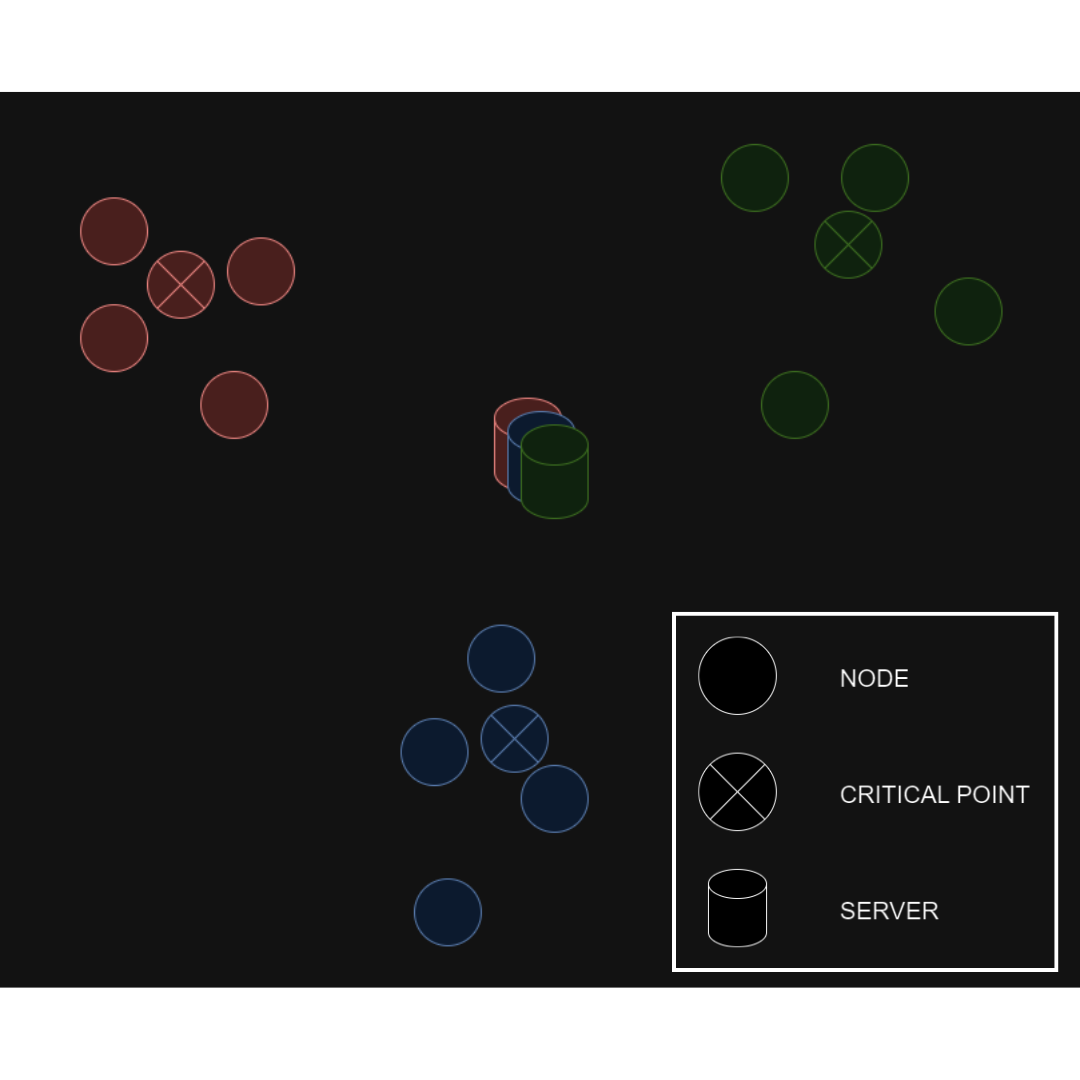
\includegraphics[width=\textwidth]{figures/chapter2/topology+ypomn.png}
    \vspace{-1cm}
    \caption{Παράδειγμα Τοπολογίας Κόμβων και Εξυπηρετητών (Κόκκινο - Φωτιά, Μπλέ - Πλημμύρα, Πράσινο - Σεισμός)}
    \label{fig46}
\end{figure}

 Ξεκινώντας από την τοπολογία του συστήματός μας, τοποθετούμε αρχικά τους εξυπηρετητές μας στο σημείο (0,0,0), στο κέντρο του οικοσυστήματός μας. Κάθε εξυπηρετητής διαθέτει $\ceil*{\frac{N}{3}}$ χρηματικά αποθέματα, με τα οποία μπορεί να προσελκύσει σε αυτόν κόμβους. Επιπλέον, θέτουμε ένα ανώτατο όριο κόμβων για κάθε εξυπηρετητή. Έτσι, κάθε εξυπηρετητής μπορεί να χτίσει ένα συνασπισμό το πολύ $\ceil*{\frac{N}{3}}$ κόμβων. Μπορεί, λοιπόν, να χρηματοδοτήσει το πολύ το $\frac{1}{3}$ των κόμβων, χαρακτηριστικό που μας βοηθά στην διατήρηση της ισορροπίας μεταξύ των εξυπηρετητών. Έπειτα, σε έναν κύβο ακμής μήκους 2, γύρω από το (0,0,0) επιλέγουμε 3 σημεία, ένα για κάθε φυσική καταστροφή. Σε αυτά θεωρούμε πως έχει συμβεί η εκάστοτε φυσική καταστροφή και άρα κόμβοι γύρω από αυτά θα έχουν χρήσιμη πληροφορία για τους εξυπηρετητές μας. Εξασφαλίζουμε επίσης πως τα σημεία δεν είναι πολύ κοντά στους εξυπηρετητές. Σε μια τέτοια περίπτωση, όπως θα δούμε και στην διαδικασία της αντιστοίχισης, οι κόμβοι γύρω από αυτό θα παρουσίαζαν πολύ μεγαλύτερη χρησιμότητα στο σύστημα, απλώς επειδή βρίσκονται κοντά στους εξυπηρετητές και είναι "φθηνή" η επικοινωνία με αυτούς. Έτσι, για να διασφαλίσουμε μια ισορροπία ορίζουμε ως ελάχιστη απόσταση από τους εξυπηρετητές $d_{min} = 0.3$. Επιπλέον, για ρεαλιστικούς κυρίως λόγους, ορίζουμε ως ελάχιστη απόσταση μεταξύ δύο κρίσιμων σημείων ίση με $d_{min} = 0.8$. 

Στη συνέχεια, μας απομένει να τοποθετήσουμε τους κόμβους μας γύρω από τα κρίσιμα σημεία. Η λογική που ακολουθούμε εδώ είναι η εξής: ανάλογα με την περιοχή που βρισκόμαστε (Αστική, Προαστιακή, Αγροτική) οι κόμβοι είναι λιγότερο ή περισσότερο αραιοί γύρω από το κάθε κρίσιμο σημείο. Συνεπώς, θέτουμε 3 όρια: $rural\_limit = 12, suburban\_limit = 21$ και $urban\_limit = 30$. Έτσι, για τις αγροτικές περιοχές όταν έχουμε πάνω από 12 κόμβους, αρχίζουμε να τοποθετούμε τους υπόλοιπους κόμβους πιο αραιά. Αντίστοιχα, το όριο για τις μικροαστικές περιοχές είναι 21 και για τις αστικές 30. Στις προσομοιώσεις μας, το μεγαλύτερο Ν που θα χρησιμοποιήσουμε είναι το $N = 30$. Επιπλέον, για δική μας διευκόλυνση ο κόμβος με διακριτικό id ανατίθεται γύρω από το κρίσιμο σημείο $id\mod3$, και όσο μεγαλύτερο το id τόσο πιο μακριά είναι από το κρίσιμο σημείο. Άρα οι τρεις πρώτοι κόμβους είναι πολύ κοντά στα κρίσιμα σημεία τους, οι τρεις επόμενοι λίγο πιο μακριά κ.ο.κ. Όπως αναφέραμε, όταν για κάθε μία από τις διαφορετικές περιοχές ξεπεράσουμε το αντίστοιχο όριο, αρχίζουμε να προσθέτουμε πιο αραιούς-μακρινούς κόμβους. Με τον τρόπο αυτό μοντελοποιούμε το γεγονός πως σε περιοχές που βρίσκονται σε προάστια ή στην εξοχή, οι γειτονικοί στο κρίσιμο σημείο κόμβοι είναι λιγότεροι, αλλά είναι πιθανό να υπάρχουν και άλλοι, όμως πιο απομακρυσμένοι, κόμβοι. Σε κάθε περίπτωση, ολοκληρώνοντας την τοπολογία μας καταλήγουμε σε 3 κρίσιμα σημεία γύρω από τους εξυπηρετητές μας, όπου το κάθε ένα έχει γύρω του κόμβους. Ανάλογα την περιοχή όπου διατίθεται το δίκτυό μας, οι κόμβοι αυτοί είναι λιγότερο ή περισσότερο αραιοί. Είναι σημαντικό να επισημάνουμε προφανώς, πως όσο πιο κοντά είναι ένας κόμβος σε ένα κρίσιμο σημείο, τόσο πιο αξιόπιστος είναι για την πληροφορία που διαθέτει για αυτό, σημαντικό χαρακτηριστικό όπως θα δούμε και στη συνέχεια για την αντιστοίχιση κόμβων-εξυπηρετητών. Τέλος, σημειώνουμε πως ο κάθε κόμβος διαθέτει δύο παραμέτρους $a_n$ και $q_n$, οι οποίες εκφράζουν τον συντελεστή αποτελεσματικής χωρητικότητας του επεξεργαστή του κόμβου και τον αριθμό κύκλων Κεντρικής Μονάδας Επεξεργασίας (ΚΜΕ) που απαιτούνται για την εκτέλεση ενός δείγματος δεδομένων αντίστοιχα.

\newpage

Παρακάτω παρουσιάζονται παραδείγματα των διαφορετικών τοπολογιών - σεναρίων: 

\begin{figure}[H]
    \centering
    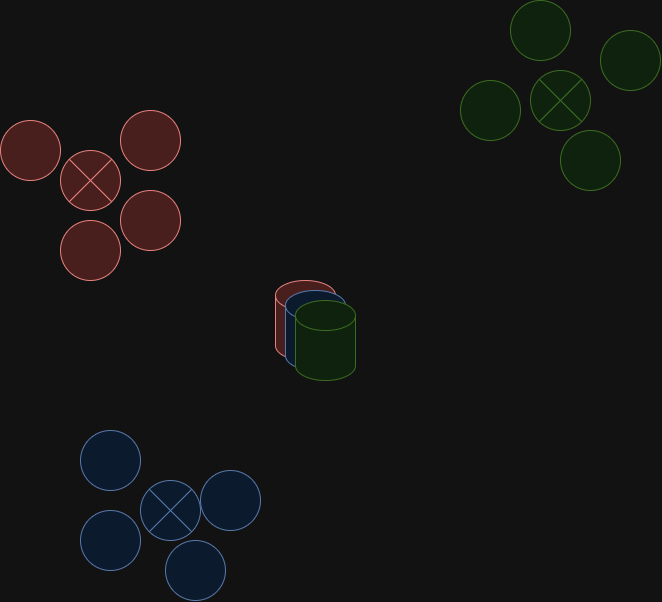
\includegraphics[width=0.7\textwidth]{figures/chapter2/urban.drawio.png}
    \caption{Αστική Περιοχή με 12 κόμβους}
    \label{fig47}
\end{figure}

\begin{figure}[H]
    \centering
    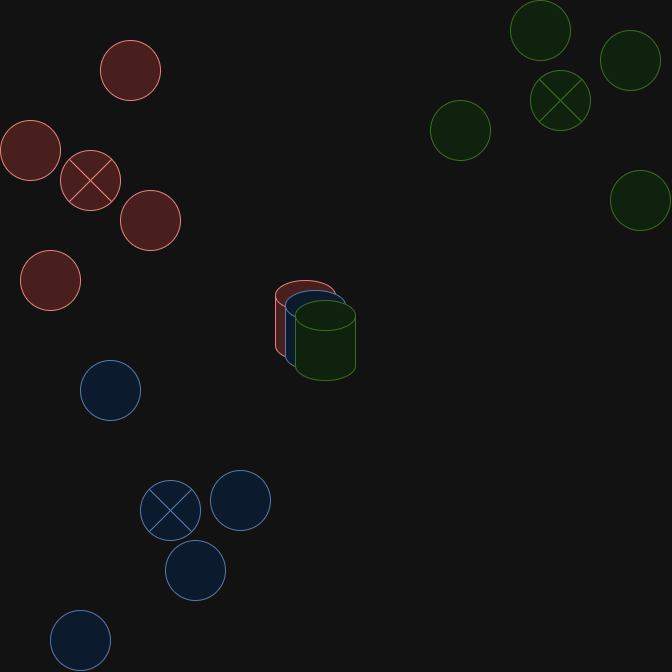
\includegraphics[width=0.7\textwidth]{figures/chapter2/suburban.drawio.png}
    \caption{Προαστιακή Περιοχή με 12 κόμβους}
    \label{fig48}
\end{figure}

\newpage

\begin{figure}[H]
    \centering
    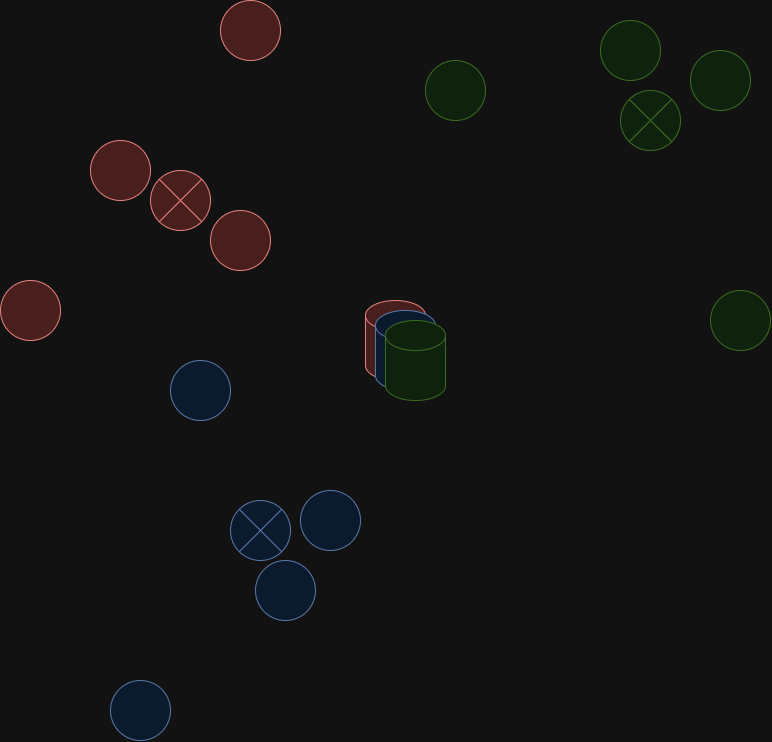
\includegraphics[width=0.7\textwidth]{figures/chapter2/rural.drawio.png}
    \caption{Αγροτική Περιοχή με 12 κόμβους}
    \label{fig49}
\end{figure}

\subsection{Υλοποίηση}

Για να συγκρίνουμε την επίδοση του αλγορίθμου μας σε διαφορετικές περιοχές (αστικό, προαστιακό ή υπαίθριο περιβάλλον) θα πρέπει να εξασφαλίσουμε μια δίκαιη και ορθή σύγκριση. Όπως αναφέραμε παραπάνω, έχουμε δύο είδη κόμβων για κάθε περιοχή, γειτονικοί - "καλοί" και απομακρυσμένοι - "κακοί". Στην αστική περιοχή και οι 30 κόμβοι, που μπορούν να μπουν ως μέγιστο όριο, θεωρούνται "καλοί" και άρα είναι σχετικά κοντά στο κρίσιμο σημείο τους. Αντίστοιχα, στην προαστιακή περιοχή μέχρι και τον 21ο κόμβο, οι κόμβοι θεωρούνται "καλοί", ενώ, σε περίπτωση που το Ν ξεπεράσει το 21, αρχίζουν να εισέρχονται στο σύστημά μας "κακοί" κόμβοι, οι οποίοι τοποθετούνται τουλάχιστον 0.2 μακριά από το κρίσιμο σημείο τους. Τέλος, στην αγροτική περιοχή, μέχρι και τον 12ο κόμβο, οι κόμβοι θεωρούνται "καλοί", ενώ, σε περίπτωση που το Ν ξεπεράσει το 12, αρχίζουν να εισέρχονται στο σύστημά μας "κακοί" κόμβοι, οι οποίοι τοποθετούνται τουλάχιστον 0.3 μακριά από το κρίσιμο σημείο τους. Συνεπώς, έστω πως έχουμε τον κόμβο i, τον οποίο θα πρέπει να δημιουργήσουμε. Αν το i είναι μικρότερο ή ίσο του 12 θα πρέπει όλες οι περιοχές να έχουν ίδιο κόμβο i και να μην ξαναδημιουργηθούν τυχαίοι κόμβοι i σε κάθε περιοχή. Με την ίδια λογική όταν το i είναι μικρότερο ή ίσο του 21 (αλλά μεγαλύτερο του 12), θα πρέπει οι κόμβοι i να είναι ίδιοι για την αστική και προαστική περιοχή, αλλά για την αγροτική περιοχή θα πρέπει να δημιουργηθεί ένας "κακός" κόμβος i. Τέλος, για διευκόλυνση μας, υπολογίζουμε και αποθηκεύουμε τις αποστάσεις κάθε κόμβου από τους εξυπηρετητές μας και την σημασία κάθε κόμβου για τον κάθε εξυπηρετητή. Τέλος, όσον αφορά τις παραμέτρους $a_n$ και $q_n$ θέτουμε:

\begin{itemize}
    \item $a_n = 2 \times 10^{(-28)} \times \text{random.uniform(0.95, 1.05)}$
    \item $q_n = 20 \times \text{random.uniform(0.95,1.05)}$
\end{itemize}

\noindent όπως αναφέρεται και σε αντίστοιχη προσομοίωση (\lcite{charatsaris2023accuracy}).

\section{Αντιστοίχιση με Θεωρία Παιγνίων}

Ως πρώτος μηχανισμός για την αντιστοίχιση κόμβων-εξυπηρετητών χρησιμοποιήθηκε η Θεωρία Παιγνίων. Στόχος ήταν να κατασκευαστεί ένα περιβάλλον με κανόνες, μέσα στο οποίο οι παίκτες-κόμβοι θα ανταγωνίζονται και θα ενεργούν για να επιτύχουν την καλύτερη δυνατή αμοιβή για εκείνους. Αντίστοιχα, οι εξυπηρετητές διαθέτοντας τους χρηματικούς πόρους τους στους κόμβους, προσπαθούν και αυτοί με τη σειρά τους να βελτιστοποιήσουν την δική τους απολαβή. Πιο αναλυτικά την διαδικασία θα περιγράψουμε παρακάτω.

\subsection{Συνάρτηση Χρησιμότητας}

Αρχικά θα πρέπει να εξηγήσουμε τον τρόπο με τον οποίο κάθε κόμβος, αλλά και εξυπηρετητής αντιλαμβάνεται το συμφέρον του στο δίκτυό μας. Έτσι χτίζουμε μία Συνάρτηση Χρησιμότητας. Κάθε κόμβος $n$ έχει μια ποσότητα συλλεγμένων δεδομένων $D_n$ [bits], και η σημασία των δεδομένων τους ορίζεται ως:

\vspace{-5pt}

\begin{equation}
c_{n,k}=\frac{\min\limits_{\forall n} ||L_n-L_k||}{||L_n-L_k||}
\label{eq1}
\end{equation}

\noindent
όπου $L_n = (x_n,y_n,z_n)$ [απόσταση σε m] και $L_k = (x_k,y_k,z_k)$ [απόσταση σε m], με $k$ το εκάστοτε κρίσιμο σημείο, αποτυπώνοντας πόσο κοντά στα κρίσιμα σημεία έχουν συλλεχθεί τα δεδομένα. Για κάθε έναν από τους τρεις εξυπηρετητές $s$ υπολογίζουμε την σημασία των δεδομένων του κάθε κόμβου ως:

\begin{equation}
c_{n,s}=\max\limits_{\forall k \in s} c_{n,k}
\label{eq2}
\end{equation}

\noindent
Όπως αναφέραμε, στην Ομοσπονδιακή Μάθηση, κάθε κόμβος $n$ εκπαιδεύει ένα τοπικό μοντέλο βασισμένο στον εξυπηρετητή $s$ που έχει επιλεγεί και αναφέρει το αποτέλεσμα της εκπαίδευσης σε αυτόν. Ο ρυθμός δεδομένων κάθε κόμβου $n$ όταν εκφορτώνει το τοπικό μοντέλο στον εξυπηρετητή $s$ δίνεται ως εξής:

\vspace{-5pt}

\begin{equation}
R_{n,s} = B \log_2(1 + \frac{g_{n,s} P_{n,s}}{\sum \limits_{n'\in s} g_{n',s}P_{n',s} + I_0}) \quad [bps]
\label{eq3}
\end{equation}

\vspace{-3pt}

\noindent
όπου $g_{n,s}$ δηλώνει το κέρδος καναλιού στη ζεύξη επικοινωνίας μεταξύ $n$ και $s$, $P_{n,s}$ [W] είναι η ισχύς εκπομπής του κόμβου, $B$ [Hz] είναι το εύρος ζώνης επικοινωνίας, και $I_0$ είναι ο λευκός προσθετικός θόρυβος (AWGN) μηδενικής μέσης τιμής. \lcite{charatsaris2023accuracy}

Η κατανάλωση ενέργειας ενός κόμβου $n$ για να εκπαιδεύσει τοπικά το επιλεγμένο παγκόσμιο μοντέλο υπολογίζεται ως εξής:

\vspace{-5pt}

\begin{equation}
E_n=\frac{a_n}{2}q_nD_nf_n^2 [J]
\label{eq4}
\end{equation}

\vspace{-3pt}

\noindent
όπου $a_n$ είναι ο συντελεστής χωρητικότητας του επεξεργαστή του κόμβου $n$, $q_n$ είναι οι κύκλοι της Κεντρικής Μονάδα Επεξεργασίας (ΚΜΕ) που απαιτούνται για την εκτέλεση ενός δείγματος δεδομένων, και $f_n$ [κύκλοι ΚΜΕ/δευτερόλεπτο] είναι η συχνότητα της ΚΜΕ της συσκευής του κόμβου $n$. \lcite{charatsaris2023accuracy} 

Η κατανάλωση ενέργειας λόγω της μετάδοσης της ενημέρωσης του τοπικού μοντέλου υπολογίζεται ως εξής:

\vspace{-5pt}

\begin{equation}
E_{n,s}=\frac{Z(\mathbf{w}n)P{n,s}}{R_{n,s}}[J]
\label{eq5}
\end{equation}

\vspace{-3pt}

\noindent
όπου $Z(\mathbf{w}_n)$ [bits] είναι τα δεδομένα των παραμέτρων του τοπικού μοντέλου $\mathbf{w}_n$ που μεταδίδονται για την ενημέρωση του κεντρικού μοντέλου του εξυπηρετητή $s$. \lcite{charatsaris2023accuracy}

Τέλος, ο κάθε κόμβος απολαμβάνει μια χρηματική απολαβή με βάση την σημασία των δεδομένων του, αλλά και με βάση τους υπόλοιπους κόμβους που ανήκουν στην ομοσπονδία του εξυπηρετητή:

\vspace{-5pt}

\begin{equation}
Pnt_{n,s}=\frac{c_{n,s}P_s}{\sum \limits_{n'\in s} c_{n',s}}
\label{eq6}
\end{equation}

\vspace{-3pt}

Κάθε κόμβος βιώνει μια χρησιμότητα από τη συμμετοχή του στη διαδικασία αντιστοίχισης κόμβων-εξυπηρετητών που εξαρτάται από: (i) τα χαρακτηριστικά επικοινωνίας, δηλαδή τον επιτευχθέντα ρυθμό δεδομένων για την αναφορά του ενημερωμένου τοπικού μοντέλου $\mathbf{w}n^i$ στον εξυπηρετητή ($\hat{R}{n,s}$), (ii) το χρηματικό εισόδημα που λαμβάνεται από τον εξυπηρετητή για την παροχή κινήτρων στον κόμβο για την εκπαίδευση του τοπικού μοντέλου ($\hat{Pnt}_{n,s}$) και το σταθερό κίνητρο πρόσληψης που παρέχεται από τον εξυπηρετητή ($\gamma$), (iii) το όφελος της εκμετάλλευσης κρίσιμων δεδομένων για την εκπαίδευση του τοπικού μοντέλου ($\hat{d_n}$), και (iv) το ενεργειακό κόστος για την εκπαίδευση του τοπικού μοντέλου και την αποστολή του στον εξυπηρετητή $(\hat{E}n+\hat{E}{n,s})$. Έτσι, η χρησιμότητα του κόμβου ορίζεται ως εξής:

\vspace{-5pt}

\begin{equation}
    U_{n,s}(D_n)=\alpha \hat{R}_{n,s} + \beta \hat{Pnt}_{n,s} +\gamma + \delta \hat{d_n} -\epsilon (\hat{E}n+\hat{E}{n,s})
    \label{eq7}
\end{equation}

\noindent
όπου ο εξυπηρετητής $s$ προσφέρει $Pnt_{n,s}$ [\$] ως χρηματικό κίνητρο στον κόμβο $n$ για την εκπαίδευση του τοπικού μοντέλου, και $\alpha, \beta, \gamma, \delta, \epsilon \in \mathbb{R}^+$. Για να διασφαλιστεί ότι όλοι οι παράγοντες είναι της ίδιας τάξης μεγέθους, αποτυπώνοντας έτσι δίκαια την επίδρασή τους στη χρησιμότητα του κόμβου, στη χρησιμότητα του κόμβου (Εξίσωση \ref{eq7}) οι $\hat{R}{n,s}, \hat{Pnt}_{n,s}, \hat{E}n$, $\hat{E}{n,s}$ και $\hat{d_n}$ δίνονται από τις εξής κανονικοποιημένες εκφράσεις:

\[\hat{R}{n,s} = \frac{R_{n,s}}{\max \limits_{\forall n, \forall s} { R_{n,s} }}, \hat{Pnt}_{n,s} = \frac{c_{n,s}P_s}{(\sum \limits_{n'\in s} c_{n',s}) \max \limits_{\forall s} P_s}, \hat{d}{n} = \frac{\sum \limits{\forall k \in K} c_{n,k} D_n}{\max \limits_{\forall n} { \sum \limits_{\forall k \in K} c_{n,k} D_n }}\]

\[\hat{E}{n} = \frac{E_{n}}{\max \limits_{\forall n} { E_{n} }},  \hat{E}{n,s} = \frac{E{n,s}}{\max \limits_{\forall n, \forall s} { E_{n,s} }}\]

Από την άλλη πλευρά, κάθε εξυπηρετητής στοχεύει στη μεγιστοποίηση της χρησιμότητας που βιώνουν οι συνδεδεμένοι κόμβοι του, λαμβάνοντας όμως υπόψη το κόστος παροχής κινήτρων πρόσληψης και τον ανταγωνισμό για την πρόσληψη από άλλους εξυπηρετητές εντός του δικτύου πολλαπλών μοντέλων Ομοσπονδιακής Μάθησης. Έτσι, η χρησιμότητα του ομοσπονδιακού εξυπηρετητή είναι:

\vspace{-5pt}

\begin{equation}
U_s(P_s, \mathbf{P_{-s}}) = \frac{\sum\limits_{\forall n\in \mathcal{N}s} U{n,s} - \zeta \hat{P}s^2}{\sum\limits_{\forall s'\neq s} \hat{P}_{s'}}
\label{eq8}
\end{equation}

\vspace{-5pt}

\noindent
όπου $\zeta \in \mathbb{R}^+$, $\mathcal{N}s$ είναι το σύνολο των κόμβων που επιλέγουν τον εξυπηρετητή $s$, και $\mathbf{P{-s}}$ είναι το διάνυσμα χρηματικών κινήτρων όλων των εξυπηρετητών εκτός από τον $s$. Σημειώνεται ότι ο κάθε εξυπηρετητής $s$ έχει διαθέσει $P_s$ χρηματικά κίνητρα τα οποία χρησιμοποιεί εξ' ολοκλήρου είτε για έναν είτε για $N_s$ κόμβους. Προφανώς, οι κόμβοι μας βλέποντας έναν σχετικά άδειο εξυπηρετητή γνωρίζουν πως συμμετέχοντας στην ομοσπονδία του θα έχουν καλύτερες απολαβές. Βάσει του διαθέσιμου προϋπολογισμού πρόσληψης $P_s$, όπως αναφέραμε, κάθε εξυπηρετητής μπορεί να προσλάβει έναν μέγιστο αριθμό κόμβων $N_s^{Max}$, που στην περίπτωσή μας είναι το $\frac{1}{3}$ του πλυθησμού N.

\subsection{Προσεγγιστική Αντιστοίχιση}

Οι κόμβοι επιλέγουν στρατηγικά εξυπηρετητές για να προσφέρουν τις υπολογιστικές τους υπηρεσίες, με στόχο να μεγιστοποιήσουν τη χρησιμότητά τους. Οι ομοσπονδιακοί εξυπηρετητές επιδιώκουν να προσλάβουν κόμβους για να βοηθήσουν στην εκπαίδευση του παγκόσμιου μοντέλου, στρατηγικά βελτιστοποιώντας την ακρίβειά τους μέσω της πρόσληψης κόμβων. Αυτό παρουσιάζει ένα σενάριο αντιστοίχισης πολλών προς έναν, όπου πολλαπλοί κόμβοι αντιστοιχίζονται με έναν εξυπηρετητή και μπορεί να μελετηθεί βάσει της θεωρίας αντιστοίχισης.

\begin{definition} \label{Definition 1} \textbf{(Παιχνίδι Αντιστοίχισης)} Τα σύνολα των κόμβων $\mathcal{N}$ και των εξυπηρετητών $\mathcal{S}$ δεν έχουν καμία τομή. Μια αντιστοίχιση $M$ είναι ένας αντιστοιχισμός των στοιχείων του $\mathcal{N}$ στα στοιχεία του $\mathcal{S}$, που ικανοποιεί τις συνθήκες: $|M(n)| \leq 1, \forall n \in \mathcal{N}$, $|M(s)| \leq N_s^{Max}, \forall s \in \mathcal{S}$, $M(n) \in \mathcal{S}$ εάν και μόνο εάν $M(s) \in \mathcal{N}$, $n \in M(s) \Leftrightarrow M(n) = s$. Εάν $M(n) = \emptyset$, ο κόμβος $n$ δεν αντιστοιχίζεται σε κανέναν εξυπηρετητή, ενώ εάν $M(s) = \emptyset$, τότε ο εξυπηρετητής $s$ δεν επιλέγεται από κανέναν κόμβο.

\end{definition}

Η Εξίσωση \ref{eq7} παρουσιάζει εξωτερικότητα (επιρροή μεγέθους και από άλλους κόμβους - $U_{n,s}$ εξαρτάται και από τις ενέργειες κάθε $n' \in N$) που προκύπτει από την επιλογή του εξυπηρετητή και από άλλους κόμβους, η οποία αποτυπώνεται στα μεγέθη του ρυθμού αποστολής δεδομένων και στις χρηματικές απολαβές, όπου οι κόμβοι ανταγωνίζονται για πόρους (εύρος ζώνης και χρηματικά κίνητρα). Επίσης, η Εξίσωση \ref{eq8} περιλαμβάνει την εξωτερικότητα του διαθέσιμου προϋπολογισμού πρόσληψης άλλων εξυπηρετητών. Η Προσεγγιστική Αντιστοίχιση αγνοεί αυτές τις εξωτερικότητες για να εδραιώσει γρήγορα μια αρχική αντιστοίχιση μεταξύ κόμβων και εξυπηρετητών. Οι Εξισώσεις \ref{eq7} και \ref{eq8} αναδιαμορφώνονται αποκλείοντας τις εξωτερικότητες που προέρχονται από την επιλογή εξυπηρετητή από τους κόμβους, ως εξής:

\vspace{-8pt}

\begin{equation}
\widetilde{U}_n(D_n)=\alpha \widetilde{\hat{R}}{n,s} + \beta \widetilde{\hat{Pnt}}_{n,s} +\gamma + \delta \hat{d_n} -\epsilon (\hat{E}n+\hat{E}{n,s})
\label{eq9}
\end{equation}

\vspace{-8pt}

\[\widetilde{R}{n,s} = B \log_2(1 + \frac{g_{n,s} P_{n,s}}{g_{n,s} P_{n,s} + I_0}) \> [bps], \>\>\> \widetilde{\hat{R}}{n,s} = \frac{\widetilde{R}{n,s}}{\max \limits_{\forall n, \forall s} { \widetilde{R}_{n,s} }}\]

\[\widetilde{\hat{E}}{n,s} = \frac{Z(\mathbf{w}n)P{n,s}}{\widetilde{\hat{R}}_{n,s}} \> [J], \>\>\> \widetilde{\hat{Pnt}}_{n,s} = \frac{c_{n,s}P_s}{\max \limits_{\forall s} P_s}\]

\vspace{-5pt}

\begin{equation}
\widetilde{U}s(P_s, \mathbf{P{-s}}) = \sum\limits_{\forall n\in N_s} \widetilde{U}_n - \zeta \hat{P}_s^2
\label{eq10}
\end{equation}

\vspace{-5pt}

\noindent
\begin{definition} \label{Definition 2} \textbf{(Σχέση Προτίμησης $<$)} Μια σχέση προτίμησης $<$ είναι μια πλήρης, αυτοπροτιμητική και μεταβατική δυαδική σχέση μεταξύ στοιχείων των συνόλων $\mathcal{N}$ και $\mathcal{S}$. Οι σχέσεις προτίμησης για έναν κόμβο (Εξίσωση \ref{eq11}) και έναν εξυπηρετητή (Εξίσωση \ref{eq12}) ορίζονται ως εξής:

\vspace{-5pt}

\begin{equation}
s >_n s' \Longleftrightarrow \widetilde{U}_n(D_n) > \widetilde{U}n(D_n)
\label{eq11}
\end{equation}

\vspace{-5pt}

\begin{equation}
n >_s n' \Longleftrightarrow \widetilde{U}s|{N_s \cup {n}} > \widetilde{U}s|{N_s \cup {n'}}
\label{eq12}
\end{equation}

\vspace{-8pt}

\end{definition}

\begin{algorithm}[h]
\caption{Αλγόριθμος Προσεγγιστικής Αντιστοίχισης} \label{algorithm 1}
\begin{algorithmic}[1]
\STATE \textbf{\underline{Είσοδος:}} ${L_n, a_n, q_n, D_n, f_n, \mathbf{w}n}{\forall n\in \mathcal{N}}, {L_k}_{\forall k \in \mathcal{K}}, \alpha,\beta,\gamma$,

\STATE \textbf{\underline{Έξοδος:}} \text{Αποτελέσματα Αντιστοίχισης} $M$
\STATE \textbf{\underline{Αρχικοποίηση:}} $\mathcal{N}^* \gets \mathcal{N}$: μη αντιστοιχισμένοι κόμβους, $\mathcal{S}_n \gets \{ s | \forall s \in \mathcal{S}\}, \forall n \in \mathcal{N}$: διαθέσιμοι εξυπηρετητές για κάθε κόμβου
\WHILE{$\mathcal{N}^* \neq \emptyset \text{ και } \mathcal{S}_n \neq \emptyset, \exists n \in \mathcal{N}^* $}
\FOR{$n \in \mathcal{N}^*$}
\STATE Ο κόμβος $n$ επιλέγει τον πιο ευνοϊκό εξυπηρετητή μεταξύ των εναλλακτικών και στέλνει πρόσκληση αντιστοίχισης βάσει της Εξίσωσης \ref{eq11}.
\ENDFOR
\FOR{$s \in \mathcal{S}$}
\IF{$(N_s \leq N_s^{\max}) \land (s$ \text{έλαβε πρόσκληση αντιστοίχισης}$)$}
\STATE Ο εξυπηρετητής $s$ επιλέγει τους πιο ευνοϊκούς κόμβους για αντιστοίχιση από αυτούς που έστειλαν πρόσκληση αντιστοίχισης βάσει της Εξίσωσης \ref{eq12}.
\STATE Διαγράφει τον $s$ από τους εναλλακτικούς εξυπηρετητές των κόμβων που έστειλαν πρόσκληση αντιστοίχισης αλλά δεν έγιναν δεκτοί.
\ENDIF
\ENDFOR
\ENDWHILE
\end{algorithmic}
\end{algorithm}
\vspace{-7pt}
Βάσει των Ορισμών \ref{Definition 1} και \ref{Definition 2}, ο Αλγόριθμος \ref{algorithm 1} περιγράφει τον Αλγόριθμο Προσεγγιστικής Αντιστοίχισης. Αυτός ο αλγόριθμος στοχεύει να φτάσει σε μια εκτιμώμενη αντιστοίχιση μεταξύ των κόμβων και των ομοσπονδιακών εξυπηρετητών γρήγορα, δίνοντας προτεραιότητα στη μεγιστοποίηση της χρησιμότητας και για τα δύο μέρη χωρίς να λαμβάνει υπόψη τις εξωτερικότητες του συστήματος στις διαδικασίες λήψης αποφάσεων τους. Η βελτίωση του αποτελέσματος του Αλγορίθμου Προσεγγιστικής Αντιστοίχισης παρουσιάζεται στη συνέχεια μέσω της ανάπτυξης της Ακριβούς Αντιστοίχισης, η οποία αντιμετωπίζει τις εξωτερικότητες που σχετίζονται με τους κόμβους και τους εξυπηρετητές.

\subsection{Ακριβής Αντιστοίχιση}

Λόγω της ύπαρξης εξωτερικοτήτων στη διαδικασία αντιστοίχισης των κόμβων και εξυπηρετητών, ο αλγόριθμος Προσεγγιστικής Αντιστοίχισης διασφαλίζει ένα γρήγορο, αλλά όχι βέλτιστο, αποτέλεσμα αντιστοίχισης εντός του παιχνιδιού αντιστοίχισης. Έτσι, εισάγουμε ένα παιχνίδι συμμαχιών για να βελτιώσουμε το αποτέλεσμα της αντιστοίχισης, εκμεταλλευόμενοι την έξοδο του αλγορίθμου Προσεγγιστικής Αντιστοίχισης και αντιμετωπίζοντας κατάλληλα τον αντίκτυπο των εξωτερικοτήτων.

\begin{definition} \label{Definition 3} \textbf{(Παιχνίδι Συμμαχίας)} Θεωρούμε ένα παιχνίδι συμμαχίας $(\mathcal{N, S}, U_s)$, όπου $\mathcal{N}$ και $\mathcal{S}$ είναι τα σύνολα των κόμβων και των ομοσπονδιακών εξυπηρετητών, αντίστοιχα. Για κάθε εξυπηρετητή $s$, υπάρχει μια συμμαχία που επιλέγεται από μια ξεχωριστή ομάδα κόμβων $\mathcal{N}_s = {1, \dots, n, \dots, N_s}$. Κάθε μεμονωμένος κόμβος επιλέγει μόνο έναν εξυπηρετητή. Η χρησιμότητα $U_s$ του εξυπηρετητή $s$ ορίζεται στην Εξίσωση \ref{eq10}.
\end{definition}

Μέσα στο πλαίσιο ενός παιχνιδιού συμμαχίας, ο στόχος μας είναι να βελτιστοποιήσουμε συλλογικά τις χρησιμότητες τόσο των ομοσπονδιακών εξυπηρετητών όσο και των κόμβων. Αυτό επιτυγχάνεται μέσω της διαμόρφωσης λεπτομερών \textit{συνθηκών μετάβασης} που καθοδηγούν στρατηγικά τους κόμβους είτε να εξέλθουν είτε να ενταχθούν σε μια συμμαχία.

\begin{definition} \label{Definition 4}\textbf{(Συνθήκες Μετάβασης)} Το παιχνίδι συμμαχίας περιλαμβάνει διάφορους τύπους Συνθηκών Μετάβασης (TC).

\noindent
\textbf{TC 1:} Για έναν κόμβου $n$ που δεν έχει επιλέξει κάποια συμμαχία ακόμα, ο $n$  εισέρχεται στην συμμαχία του $s$ αν 
$\exists s^* = \underset{s^* \in \mathcal{S}}{\mathrm{argmax}}\{U_{s^*} (\mathcal{N}_{s^*} \cup \{n\}) - U_{s^*}(\mathcal{N}_{s^*}) \mid U_{s^*} (\mathcal{N}_{s^*} \cup \{n\}) - U_{s^*}(\mathcal{N}_{s^*}) > 0\}$.

\noindent
\textbf{TC 2:} Ο κόμβος $n \in \mathcal{N}_s, n$ φεύγει από τον εξυπηρετητή $s$ αν $U_s(\mathcal{N}_{s} \setminus \{n\}) > U_s(\mathcal{N}_{s})$, και άρα,  $M = \{M \setminus \{\mathcal{N}_{s}\}\} \cup \{\mathcal{N}_{s} \setminus \{n\}\}$.

\noindent
\textbf{TC 3:} Ο κόμβος $n \in \mathcal{N}_{s}$, αποχωρεί από την συμμαχία του εξυπηρετητή του $s$ και επιλέγει την συμμαχία του εξυπηρετητή $s' \neq s$ αν $U_s(\mathcal{N}_{s} \setminus \{n\}) + U_{s'}(\mathcal{N}_{s'} \cup \{n\}) > U_s(\mathcal{N}_{s}) + U_{s'}(\mathcal{N}_{s'})$, και άρα, $M = \{M \setminus \{\mathcal{N}_s,\mathcal{N}_{s{'}}\}\} \cup \{\mathcal{N}_{s}  \setminus \{n\}\} \cup \{\mathcal{N}_{s'}  \cup \{n\}\}$.

\noindent
\textbf{TC 4:} Ο κόμβος $n\in \mathcal{N}_{s}$ και ο κόμβος $n' \in \mathcal{N}_{s'}, n \neq n'$, $n$ and $n'$ αλλάζουν συμμαχίες μεταξύ τους αν $U_s((\mathcal{N}_{s} \setminus \{n\}) \cup \{n'\}) + U_{s'}((\mathcal{N}_{s'} \setminus \{n'\} )\cup \{n\}) > U_s(\mathcal{N}_{s}) + U_{s'}(\mathcal{N}_{s'})$, και άρα, $M = \{M \setminus \{\mathcal{N}_s,\mathcal{N}_{s{'}}\}\} \cup \{(\mathcal{N}_{s}  \setminus \{n\}) \cup \{n'\}\} \cup \{(\mathcal{N}_{s'}  \setminus \{n'\}) \cup \{n\}\}$.
\end{definition}

Βάσει των συνθηκών μετάβασης που περιγράφονται στον Ορισμό \ref{Definition 4}, έχουμε αναπτύξει τον Αλγόριθμο Ακριβούς Αντιστοίχισης \ref{algorithm 2}. Ο Αλγόριθμος Ακριβούς Αντιστοίχισης έχει σχεδιαστεί για να διευκολύνει την καθιέρωση σταθερών συμμαχιών μεταξύ κόμβων και εξυπηρετητών και θα αποδείξουμε την ιδιότητά του αυτή αφού παρουσιάσουμε τον αλγόριθμο.

\begin{algorithm}[h]
\caption{Αλγόριθμος Ακριβούς Αντιστοίχισης} \label{algorithm 2}
\begin{algorithmic}[1]
\STATE \textbf{\underline{Είσοδος:}}
    $M_{\text{initial}}$ από τον Αλγόριθμο Προσεγγιστικής Αντιστοίχισης, και ίδιες εισόδους με τον Αλγόριθμο Προσεγγιστικής Αντιστοίχισης
\STATE \textbf{\underline{Έξοδος:}}
    Βέλτιστος Διαμοιρασμός Συνασπισμών $M^*$
    \REPEAT
        \STATE Τυχαία επιλογή κόμβου $n$ και συνασπισμού εξυπηρετητή $s$
        \IF {$n$ δεν ανήκει σε κανένα συνασπισμό}
            \STATE $s^* = \underset{s^* \in M}{\text{argmax}} \{ (U_{s^*}(\mathcal{N}_{s^*}\cup\{n\}) - U_{s^*}(\mathcal{N}_{s^*}) | U_{s^*}(\mathcal{N}_{s^*}\cup\{n\}) - U_{s^*}(\mathcal{N}_{s^*}) > 0) \land (N_s \leq N_s^{\max})\}$
            \STATE $M = \{M \setminus\{n\}\} \cup \{\mathcal{N}_s\cup\{n\}\}$
        \ELSE
            \STATE Διαλέγουμε τυχαία  $s', s' \neq s$ 
            \IF{$N_s \leq N_s^{\max}$}
                \IF {$U_s( \mathcal{N}_s \setminus \{n\}) + U_{s'}(\mathcal{N}_{s{'}} \cup \{n\}) > U_s(\mathcal{N}_s) + U_{s'}(\mathcal{N}_{s{'}})$}
                    \STATE $M = \{M \setminus\{\mathcal{N}_s,\mathcal{N}_{s{'}}\}\}\cup\{\mathcal{N}_s\setminus\{n\}\}\cup\{\mathcal{N}_{s{'}}\cup\{n\}\}$
                \ENDIF
            \ELSE
                \STATE Διαλέγουμε τυχαία κόμβου $n'$ από τον συνασπισμό του εξυπηρετητή $s'$
                \IF {$U_s((\mathcal{N}_s \setminus \{n\})\cup\{n'\}) + U_{s'}((\mathcal{N}_{s'}\setminus\{n'\})\cup\{n\}) > U_s(\mathcal{N}_s) + U_{s'}(\mathcal{N}_{s'})$}
                    \STATE $M=\{M\setminus \{\mathcal{N}_s,\mathcal{N}_{s'}\}\} \cup \{(\mathcal{N}_s \setminus \{n\}) \cup \{n'\}\} \cup \{(\mathcal{N}_{s'} \setminus\{n'\}) \cup \{n\}\}$
                \ENDIF
            \ENDIF
        \ENDIF
        \STATE Ενημερώνουμε τους $s$ και $n$ πως πλέον ο $n$ ανήκει στον συνασπισμό του $s$
        \IF {$U_s(\mathcal{N}_s\setminus\{n\}) > U_s(\mathcal{N}_s)$}
            \STATE $M = \{M \setminus \{\mathcal{N}_s\}\} \cup \{\mathcal{N}_s\setminus\{n\}\}$
        \ENDIF
    \UNTIL{να μην έχουμε αλλαγές στην κατάσταση των κόμβων}
\end{algorithmic}
\end{algorithm}

\label{Theorem 1} \textbf{Nash-Ατομικά Σταθερός Χωρισμός κόμβων}: Ένας χωρισμός των κόμβων σε συμμαχίες με ομοσπονδιακούς εξυπηρετητές, που σημειώνεται ως $M^*$, θεωρείται Nash-Ατομικά σταθερός αν κανένας μεμονωμένος κόμβος δεν μπορεί να αυξήσει τη χρησιμότητά του αλλάζοντας εξυπηρετητές (\lcite{osborne1994game}). Ο Αλγόριθμος Ακριβούς Αντιστοίχισης είναι σχεδιασμένος να εγγυάται τουλάχιστον έναν Νας-Ατομικά σταθερό χωρισμό $M^*$.

Αρχικά, υποθέτουμε ότι το $M^*$ όπως καθορίζεται από τον Αλγόριθμο Ακριβούς Αντιστοίχισης δεν είναι Νας-Ατομικά σταθερό. Τότε, τουλάχιστον μία από τις ακόλουθες συνθήκες πρέπει να ισχύει: 

\begin{enumerate}
    \item $\exists n \notin \mathcal{N}_s, \forall s \in \mathcal{S},  \exists s^* = \underset{s^* \in \mathcal{S}}{\text{argmax}} \{U_{s^*}( \mathcal{N}_{s^*} \cup \{n\}) - U_{s^*}(\mathcal{N}_{s^*}) | U_{s^*}(\mathcal{N}_{s^*}\cup \{n\}) - U_{s^*}( \mathcal{N}_{s^*}) > 0\}$
    \item $\exists n \in \mathcal{N}_s$, που ικανοποιεί $U_{s}(\mathcal{N}_{s}\setminus\{n\})> U_{s}(\mathcal{N}_{s})$
    \item $\exists n \in \mathcal{N}_{s}, \exists s', s \neq s'$, που ικανοποιεί $U_{s}(\mathcal{N}_{s} \setminus \{n\}) + U_{s'}(\mathcal{N}_{s'}\cup\{n\})>U_{s}(\mathcal{N}_{s}) +U_{s'}(\mathcal{N}_{s'})$
    \item $\exists n \in \mathcal{N}_{s}$, $\exists n' \in \mathcal{N}_{s'}$, and $s \neq s'$, που ικανοποιεί $U_{s}((\mathcal{N}_{s} \setminus \{n\})\cup\{n'\}) + U_{s'}((\mathcal{N}_{s'}\setminus\{n'\})\cup\{n\})>U_{s}(\mathcal{N}_{s}) +U_{s'}(\mathcal{N}_{s'})$
\end{enumerate}

Ωστόσο, στον Αλγόριθμο Ακριβούς Αντιστοίχισης, αν ισχύει οποιαδήποτε από τις παραπάνω συνθήκες, οι κόμβοι θα ακολουθήσουν τις αντίστοιχες συνθήκες μετάβασης που περιγράφονται στον Ορισμό \ref{Definition 4}. Έτσι, ο χωρισμός των κόμβων δεν μπορεί να είναι τελικός, καθώς θα συνεχίσουν να τροποποιούν τους εξυπηρετητές με τους οποίους συνδέονται ακολουθώντας αυτές τις συνθήκες μετάβασης. Αυτή η αντίφαση αμφισβητεί την αρχική μας υπόθεση, οδηγώντας στο συμπέρασμα ότι ο Αλγόριθμος Ακριβούς Αντιστοίχισης συγκλίνει σε μια Nash-Ατομικά σταθερή διαμόρφωση συμμαχιών.

\subsection{Υλοποίηση}

Στο πλαίσιο της υλοποίησης των παραπάνω αλγορίθμων, για την μελέτη της βέλτιστης αντιστοίχισης, τρέχουμε τον παραπάνω αλγόριθμο για ορισμένο πλήθος επαναλήψεων συλλέγοντας πληροφορία για τις προτημήσεις και τη συμπεριφορά του κάθε κόμβου. Έτσι ανάλογα με την επιλογή και ενέργεια του τυχαίου κόμβου που επιλέγεται σε κάθε επανάληψη , αυτός παίρνοντας ανατροφοδότηση, συλλέγει μια αμοιβή από το περιβάλλον του. Συνεπώς, με την ολοκλήρωση της διαδικασίας, κάθε κόμβος έχει συλλέξει συνολική πληροφορία για τις επιλογές που διαθέτει και άρα πλέον γνωρίζει τις προτιμότερες επιλογές του. Έτσι, οι κόμβοι, σεβόμενοι το μέγιστο πλήθος κόμβων που μπορεί να υποστηρίξει κάθε εξυπηρετητής, επιλέγουν τον καλύτερο για αυτούς εξυπηρετητή.

\section{Ομοσπονδιακή Μάθηση}

Με την ολοκλήρωση της αντιστοίχισης των κόμβων με τους εξυπηρετητές, σειρά έχει η διαδικασία της Ομοσπονδιακής Μάθησης για την επίτευξη της εκπαίδευσης των μοντέλων. Εξάλλου, μας αφορά η καλή λειτουργεία της αντιστοίχισης ώστε να μπορέσουμε να επιτύχουμε καλύτερα αποτελέσματα στις αποδόσεις των μοντέλων των εξυπηρετητών, εκμεταλλευόμενοι τα δεδομένα των κόμβων με βάση τα χαρακτηριστικά του καθενός. Ας περιγράψουμε σύντομα την γενική διαδικασία της Ομοσπονδιακής Μάθησης μεταξύ κόμβων και ενός εξυπηρετητή. 

Η διαδικασία ξεκινά με έναν κεντρικό εξυπηρετητή να αρχικοποιεί ένα παγκόσμιο μοντέλο, το οποίο διανέμεται σε όλους τους συμμετέχοντες κόμβους. Κάθε κόμβος εκπαιδεύει στη συνέχεια το μοντέλο τοπικά χρησιμοποιώντας το δικό του σύνολο δεδομένων, ενημερώνοντας τις παραμέτρους του μοντέλου μέσω αρκετών επαναλήψεων. Μετά την τοπική εκπαίδευση, οι κόμβοι στέλνουν τα ενημερωμένα βάρη των μοντέλων τους πίσω στον εξυπηρετητή, ο οποίος συγκεντρώνει αυτές τις ενημερώσεις για να σχηματίσει ένα νέο κεντρικό μοντέλο. Αφού ο εξυπηρετητής ενημερώσει το κεντρικό μοντέλο με βάση τα βάρη που έλαβε από τους κόμβους, το αναδιανέμει στη συνέχεια πίσω σε αυτούς, και η διαδικασία επαναλαμβάνεται για πολλούς γύρους μέχρι να επιτευχθεί η επιθυμητή ακρίβεια του μοντέλου. Αυτή η μέθοδος διασφαλίζει ότι τα ευαίσθητα δεδομένα δεν φεύγουν ποτέ από τις τοπικές συσκευές, μειώνοντας τον κίνδυνο παραβιάσεων δεδομένων και αξιοποιώντας τους τοπικούς υπολογιστικούς πόρους των κόμβων για κατανεμημένη εκπαίδευση του μοντέλου. Ωστόσο, η Ομοσπονδιακή Μάθηση αντιμετωπίζει προκλήσεις όπως ετερογενείς κατανομές δεδομένων και μεταβλητότητα συστήματος μεταξύ των κόμβων.

\subsection{Περιγραφή}

Κάθε ένας από τους εξυπηρετητές με τον συνασπισμό του, λοιπόν, ακολουθεί πιο αναλυτικά τις παρακάτω δύο φάσεις:

\textbf{Τοπική Εκπαίδευση και Ενημέρωση Μοντέλου:} Με την έναρξη της διαδικασίας της Ομοσπονδιακής Μάθησης, κάθε κόμβος $n$ ανακτά το συγκεντρωτικό μοντέλο από τον επιλεγμένο εξυπηρετητή. Στη συνέχεια, το τοπικό μοντέλο υποβάλλεται σε επαναληπτική εκπαίδευση χρησιμοποιώντας το αντίστοιχο τοπικό σύνολο δεδομένων $D_n$. Η ενημέρωση του τοπικού μοντέλου σε κάθε κόμβο διαρκεί για έναν προκαθορισμένο αριθμό $I$ επαναλήψεων πριν προχωρήσει στη επόμενη φάση. Ορίζοντας $i$ ως την επανάληψη της ενημέρωσης του τοπικού μοντέλου στη συσκευή του κόμβου, ο κύριος στόχος για κάθε κόμβο $n$ στην $i$-οστή τοπική επανάληψη είναι να ελαχιστοποιήσει τη συνάρτηση εμπειρικής απώλειας $F_n(\mathbf{w}_n^i)$:

\vspace{-5pt}

\begin{equation}
   \mathbf{w}_n^i=\argmin\limits_{\mathbf{w}_n^i} \{F_n(\mathbf{w}_n^i)=\frac{1}{D_n}\sum\limits_{\forall j\in D_n}f_j(\mathbf{w}_n^i)\}
    \label{eq13}
\end{equation}

\vspace{-5pt}

\noindent
όπου $\mathbf{w}_n^i$ τα τοπικά βάρη του κόμβου $n$ στην i-οστή τοπική επανάληψη και $f_j(\mathbf{w}_n^i)$ η συνάρτηση απώλειας του δείγματος $j$.

Η διαδικασία επαναληπτικής ενημέρωσης εντός κάθε κόμβου μπορεί να εκτελεστεί μέσω της εφαρμογής καθόδου στοχαστικής κλίσης σε mini-batches που δειγματοληπτούνται τυχαία από το τοπικό σύνολο δεδομένων:

\vspace{-5pt}
\begin{equation}
   \mathbf{w}_n^i=\mathbf{w}_n^{i-1}-\lambda \nabla F_n(D_n \mathbf{w}_n^{i-1})
    \label{eq14}
\end{equation}

\vspace{-5pt}

\noindent
όπου $\lambda \in (0,1)$ είναι ο ρυθμός εκμάθησης της εκπαίδευσης.

\textbf{Συγκέντρωση Παγκόσμιου Μοντέλου:} Μετά από $I$ επαναλήψεις, κάθε εξυπηρετητής συγκεντρώνει τις τοπικές ενημερώσεις από τους επιλεγμένους κόμβους και αντικαθιστά το κεντρικό μοντέλο με το μέσο μοντέλο, ως ο κατά βάρος μέσος όρος των παραμέτρων του μοντέλου κάθε κόμβου. Τα βάρη προκύπτουν ως την κανονικοποιημένη σημασία του κάθε κόμβου για τον εξυπηρετητή στον οποίο ανήκει. Έτσι προκύπτει:

\vspace{-5pt}

\begin{equation}
   \mathbf{w}_s = \hat{g}_n \mathbf{w}_n^i, \quad \hat{g}_n = \frac{g_n}{\sum\limits_{\forall n \in \mathcal{N}_s} g_n}, \quad g_n = \frac{c_{n,s}}{\sum\limits_{\forall n \in N_s} c_{n,s}}
    \label{eq15}
\end{equation}

\vspace{-5pt}

Στη συνέχεια, το τοπικό μοντέλο κάθε κόμβου $\mathbf{w}_n^i$ ενημερώνεται με το κεντρικό μοντέλο $\mathbf{w}_s$ από τον εξυπηρετητή με τον οποίο είναι συνδεδεμένος ο κόμβος. Η συγκέντρωση των βαρών των κόμβων στο κεντρικό μοντέλο επαναλαμβάνεται για $\kappa$ επαναλήψεις μέχρι να επιτευχθεί η επιθυμητή ακρίβεια.

\subsection{Σύνολο δεδομένων}

Όσον αφορά τα δεδομένα των κόμβων, αναφέραμε πως κάθε ένας διαθέτει στο σύνολο δεδομένων του εικόνες σχετικές με τις κοντινές του φυσικές καταστροφές, αλλά και εικόνες από την καθημερινή ζωή. Άρα έχουμε 4 ειδών ετικέτες: φωτιά, πλημμύρα, σεισμός και ουδέτερο. Προφανώς κάθε εξυπηρετητής ενδιαφέρεται για μία μόνο φυσική καταστροφή και άρα οι τελικές ετικέτες για κάθε εξυπηρετητή και τον συνασπισμό του είναι "my\_disaster" ή "other". Οπότε έχουμε για κάθε εξυπηρετητή ένα πρόβλημα δυαδικής ταξινόμησης.

Οι εικόνες των φυσικών καταστροφών που χρησιμοποιήθηκαν, αποτελούν συνένωση συνόλων δεδομένων που βρέθηκαν στην πλατφόρμα του kaggle, ενώ το τροποποιημένο και συννενωμένο σύνολο μπορείτε να δείτε \href{https://www.kaggle.com/datasets/georgemystriotis/disasters-dataset}{\underline{εδώ}}. Οι εικόνες αποτελούν φωτογραφίες από κοντινά πλάνα σε καταστροφές, όπως φωτογραφίες από κινητά τηλέφωνα περαστικών ή πλάνα από ειδησεογραφική κάλυψη (Δεν χρησιμοποιήθηκαν αεροφωτογραφίες, για να υπάρχει ομοιογένεια στα δεδομένα).

Σε κάθε κόμβο ανατίθονται 250 ουδέτερες εικόνες, ενώ ανάλογα με το πόσο κοντά βρίσκεται στα κρίσιμα σημεία του ανατίθονται εικόνες από τις φυσικές καταστροφές. Εάν ένας κόμβος βρίσκεται περισσότερο από 0.4 μακριά από ένα κρίσιμο σημείο, υποθέτουμε πως δεν διαθέτει πληροφορίες για αυτό. Επιπλέον, κάθε εξυπηρετητής διαθέτει ένα δικό του μικρό σύνολο δεδομένων με 250 ουδέτερες φωτογραφίες και 250 φωτογραφίες της καταστροφής που το αφορά, έτσι ώστε να συμμετέχει και αυτός στην εκπαίδευση του κεντρικού του μοντέλου.

Τέλος, για να μελετήσουμε διαφοροποιήσεις μεταξύ των διάφορων εξυπηρετητών, εφαρμόζουμε τον διαμοιρασμό των εικόνων στους κόμβους εξασφαλίζοντας ότι συνολικά: $D_{fire} > D_{flood} > D_{earthquake}$. Ο διαμοιρασμός αυτός, θα μας επιτρέψει να δούμε τις διαφορές μεταξύ των αποτελεσμάτων των διαφορετικών προβλημάτων και να καταλάβουμε την επίδραση των επιπλέον κόμβων ή επιπλέον δεδομένων σε κάθε περίπτωση.

\subsection{Μοντέλο - Εκπαίδευση}

Το μοντέλο που χρησιμοποιήθηκε για κάθε εξυπηρετητή αποτελείται από ένα προ-εκπαιδευμένο μοντέλο με δύο επίπεδα απόφασης στα κορυφαία στρώματα. Το μοντέλο αυτό θα πρέπει να μπορεί να εκπαιδευτεί και να λειτουργήσει αποδοτικά σε συσκευές που δεν είναι απαραίτητα ισχυρές υπολογιστικά (ασθενής Κεντρική Μονάδα Επεξεργασίας - ΚΜΕ και έλλειψη επιταχυντών). Συνεπώς ως προ-εκπαιδευμένο μοντέλο επιλέχθηκε το MobileNetV3 το οποίο έχει μικρό μέγεθος και εκπαιδεύεται με ικανοποιητικές ταχύτες σε ΚΜΕ (χωρίς επιταχυντές), αλλά και σε κινητά τηλέφωνα.

Πιο αναλυτικά, το MobileNetV3 είναι ένα προηγμένο συνελικτικό νευρωνικό δίκτυο σχεδιασμένο ειδικά για εφαρμογές σε κινητές συσκευές, όπου οι υπολογιστικοί πόροι και η κατανάλωση ενέργειας είναι περιορισμένοι. Χτίζει πάνω στις αρχές των προκατόχων του, MobileNetV1 και MobileNetV2, και εισάγει πολλές σημαντικές καινοτομίες για την ενίσχυση της απόδοσης (\lcite{howard2019mobilenetv3}). Χτίζει πάνω στις αρχές των προκατόχων του, MobileNetV1 και MobileNetV2, και εισάγει πολλές σημαντικές καινοτομίες για την ενίσχυση της απόδοσης. Ένα βασικό χαρακτηριστικό που κληρονομήθηκε από το MobileNetV1 είναι οι κατά βάθος διαχωριζόμενες συνελίξεις, μια μέθοδος που διαχωρίζει τη συμβατική επιχείρηση σύγκλισης σε δύο διακριτά στάδια: κατά βάθος σύγκλιση και κατά σημείο σύγκλιση. Αυτός ο διαχωρισμός μειώνει σημαντικά τον αριθμό των παραμέτρων και το υπολογιστικό κόστος, καθιστώντας το δίκτυο πιο αποδοτικό. Η κατά βάθος σύγκλιση επεξεργάζεται κάθε κανάλι εισόδου ανεξάρτητα, ενώ η κατά σημείο σύγκλιση συνδυάζει αυτά τα κανάλια εξόδου, επιτρέποντας στο δίκτυο να συλλαμβάνει σύνθετα χαρακτηριστικά χωρίς το υπολογιστικό βάρος των παραδοσιακών συγκλίσεων. Επιπλέον, το MobileNetV3 ενσωματώνει την έννοια των ανεστραμμένων υπολειμάτων από το MobileNetV2. Τα ανεστραμμένα υπολείματα χρησιμοποιούν έναν συνδυασμό ελαφρών κατά βάθος διαχωριζόμενων συνελίξεων ακολουθούμενων από μια γραμμική συμφόρηση, η οποίο βοηθά στη διατήρηση των βασικών πληροφοριών χαρακτηριστικών, ενώ διατηρεί την πολυπλοκότητα του μοντέλου υπό έλεγχο (\lcite{howard2019mobilenetv3}). Αυτός ο σχεδιασμός διατηρεί μια ισορροπία μεταξύ υπολογιστικής αποδοτικότητας και αποτελεσματικής αναπαράστασης χαρακτηριστικών, εξασφαλίζοντας ότι το MobileNetV3 παραμένει τόσο ισχυρό όσο και αποδοτικό σε πόρους.

Το MobileNetV3 χρησιμοποιεί αποδοτικές αρχιτεκτονικές τεχνικές, όπως οι διαχωρίσιμες συνελίξεις σε βάθος (depthwise separable convolutions), ενώ ενσωματώνει προηγμένες τεχνικές, όπως τα μπλοκ Squeeze-and-Excitation (SE), για την ενίσχυση της δυνατότητας αναπαράστασης των συνελικτικών νευρωνικών δικτύων. Οι διαχωρίσιμες συνελίξεις σε βάθος έχουν σχεδιαστεί για να μειώνουν το υπολογιστικό κόστος και τον αριθμό των παραμέτρων σε ένα νευρωνικό δίκτυο χωρίς να θυσιάζουν σημαντικά την ακρίβεια. Αυτό είναι ιδιαίτερα χρήσιμο για ελαφριά μοντέλα όπως το MobileNet, τα οποία προορίζονται για κινητές και ενσωματωμένες συσκευές. Τα SE μπλοκς (Squeeze-and-Excitation) αποτελούν ένα εξελιγμένο αρχιτεκτονικό στοιχείο σχεδιασμένο για να ενισχύσει τη δυνατότητα αναπαράστασης των συνελικτικών νευρωνικών δικτύων (\lcite{hu2018squeeze}). Το SE μπλοκ λειτουργεί δυναμικά ανακατανέμοντας τις αντιδράσεις χαρακτηριστικών κατά κανάλια, επιτρέποντας στο δίκτυο να επικεντρωθεί σε πιο σημαντικά χαρακτηριστικά. Αυτό επιτυγχάνεται μέσω μιας διαδικασίας δύο βημάτων: πρώτα, εκτελεί παγκόσμια μέση προσαρμογή (global average pooling) για να δημιουργήσει στατιστικά στοιχεία κατά κανάλια, "στριμώχνοντας" αποτελεσματικά τις χωρικές πληροφορίες σε μια συμπαγή αναπαράσταση. Στη συνέχεια, εφαρμόζει μια σειρά πλήρως συνδεδεμένων στρωμάτων με συνάρτηση ενεργοποίησης την σιγμοειδή, για να "ενεργοποιήσει" ή να ανακατανείμει αυτά τα στατιστικά στοιχεία κατά κανάλια, τονίζοντας πιο σχετιζόμενα χαρακτηριστικά ενώ καταστέλλει τα λιγότερο σημαντικά. Αυτή η ανακατανομή βοηθά το δίκτυο να μάθει πιο αποτελεσματικά, ενισχύοντας την ευαισθησία του σε σημαντικά χαρακτηριστικά και βελτιώνοντας τη συνολική απόδοση. Ενσωματώνοντας μπλοκ SE, τα μοντέλα μπορούν να επιτύχουν υψηλότερη ακρίβεια και καλύτερη γενίκευση, καθιστώντας τα ιδιαίτερα πολύτιμα σε σύνθετα καθήκοντα όπου η διάκριση χαρακτηριστικών είναι κρίσιμη.

Το μοντέλο χρησιμοποιεί επίσης μια νέα συνάρτηση ενεργοποίησης, τη hard-swish, η οποία παρέχει μια υπολογιστικά αποδοτική εναλλακτική λύση στη συνάρτηση swish, συμβάλλοντας τόσο στη βελτίωση της απόδοσης όσο και στη γρηγορότερη εκτέλεση (\lcite{ramachandran2017swish}). Η συνάρτηση ενεργοποίησης Swish ορίζεται ως
\[
\text{swish}(x) = x \cdot \sigma(x),
\]
όπου \(\sigma(x)\) είναι η σιγμοειδής συνάρτηση
\[
\sigma(x) = \frac{1}{1 + e^{-x}}.
\]
Η συνάρτηση Swish χαρακτηρίζεται από τη λείότητα και τη μη μονοτονία της, γεγονός που της επιτρέπει να κλιμακώνει και να μετατοπίζει προσαρμοστικά την είσοδο, βελτιώνοντας έτσι την απόδοση σε ορισμένα καθήκοντα βαθιάς μάθησης σε σύγκριση με παραδοσιακές συναρτήσεις ενεργοποίησης όπως η ReLU. Αυτή η συνάρτηση επιτρέπει στα νευρωνικά δίκτυα να μάθουν πιο σύνθετες και πλούσιες αναπαραστάσεις, ενισχύοντας την απόδοσή τους.

Αντίθετα, η συνάρτηση Hard-Swish είναι μια υπολογιστικά αποδοτική προσεγγιστική συνάρτηση της Swish, οριζόμενη ως
\[
\text{hard-swish}(x) = x \cdot \text{ReLU6}(x + 3) / 6,
\]
όπου \(\text{ReLU6}(x)\) είναι η συνάρτηση ReLU6
\[
\text{ReLU6}(x) = \min(\max(0, x), 6).
\]

Η Hard-Swish είναι μια τμηματικά γραμμική συνάρτηση που προσεγγίζει τη Swish, ενώ είναι λιγότερο υπολογιστικά απαιτητική. Χρησιμοποιώντας τη Hard-Swish, το MobileNetV3 επωφελείται από ταχύτερους χρόνους επαγωγής και μειωμένα υπολογιστικά κόστη χωρίς σημαντική απώλεια ακρίβειας σε σύγκριση με τη χρήση της Swish άμεσα.

Η αρχιτεκτονική επωφελείται από μια αυτοματοποιημένη Αναζήτηση Νευρωνικής Αρχιτεκτονικής (NAS) που βελτιστοποιεί τόσο για καθυστέρηση όσο και για ακρίβεια, με αποτέλεσμα ένα δίκτυο που ισορροπεί υψηλή ακρίβεια με χαμηλό υπολογιστικό κόστος (\lcite{zoph2016nas}). Η Αναζήτηση Αρχιτεκτονικής Νευρωνικών Δικτύων είναι μια προηγμένη τεχνική μηχανικής μάθησης σχεδιασμένη για την αυτόματη ανακάλυψη βέλτιστων αρχιτεκτονικών νευρωνικών δικτύων. Αντί για χειροκίνητη σχεδίαση των δομών των δικτύων, η μέθοδος Αναζήτησης Αρχιτεκτονικής Νευρωνικών Δικτύων χρησιμοποιεί αλγόριθμους για να εξερευνήσει και να αξιολογήσει διάφορες αρχιτεκτονικές διαμορφώσεις προκειμένου να εντοπίσει το πιο αποτελεσματικό σχέδιο για μια συγκεκριμένη εργασία. Η διαδικασία Αναζήτησης Αρχιτεκτονικής Νευρωνικών Δικτύων περιλαμβάνει τον καθορισμό ενός χώρου αναζήτησης, ο οποίος περιέχει δυνητικά επίπεδα δικτύου, συνδέσεις και υπερπαραμέτρους, και την εφαρμογή μιας στρατηγικής αναζήτησης που χρησιμοποιεί αλγόριθμους όπως η ενισχυτική μάθηση, οι εξελικτικές μέθοδοι ή τεχνικές βασισμένες σε βαθμούς για να εξερευνήσει συστηματικά αυτόν τον χώρο. Στη συνέχεια, γίνεται εκτίμηση απόδοσης και αξιολόγησης των υποψήφιων αρχιτεκτονικών με βάση μετρικές όπως η ακρίβεια και η υπολογιστική αποδοτικότητα. Τα οφέλη της NAS περιλαμβάνουν τη βελτιστοποιημένη απόδοση, καθώς μπορεί να ισορροπήσει την ακρίβεια και την υπολογιστική αποδοτικότητα και να δώσει εξατομικευμένες λύσεις προσαρμοσμένες σε συγκεκριμένες εργασίες και περιορισμούς. 

Στην περίπτωση του MobileNetV3, η NAS χρησιμοποιήθηκε για να τελειοποιήσει την αρχιτεκτονική προκειμένου να επιτευχθεί μια βέλτιστη ισορροπία μεταξύ καθυστέρησης και ακρίβειας, με αποτέλεσμα ένα μοντέλο που διατηρεί υψηλή απόδοση ενώ ελαχιστοποιεί το υπολογιστικό κόστος. Αυτό καθιστά το MobileNetV3 ιδιαίτερα αποτελεσματικό για εφαρμογές σε περιβάλλοντα με περιορισμένους πόρους, όπως οι κινητές συσκευές.

Διαθέσιμο σε δύο παραλλαγές, MobileNetV3-Large και MobileNetV3-Small, είναι κατάλληλο για διάφορες εφαρμογές, συμπεριλαμβανομένων της επεξεργασίας εικόνας και βίντεο σε πραγματικό χρόνο, επαυξημένης πραγματικότητας (AR), εικονικής πραγματικότητας (VR), ενσωματωμένων συστημάτων και αυτόνομων οχημάτων. Συνολικά, το MobileNetV3 προσφέρει μια ελαφριά αλλά ισχυρή λύση για την ανάπτυξη μοντέλων βαθιάς μάθησης σε συσκευές με περιορισμένους πόρους.

Στην περίπτωσή μας χρησιμοποιήθηκε το μοντέλο MobileNetV3-Large για την Εξαγωγή των Χαρακτηριστικών των εικόνων που χρησιμοποιούνται κάθε φορά στην εκπαίδευση. Σε κάθε επανάληψη της εκπαίδευσης τα χαρακτηριστικά περνούν από ένα ισοπεδωτικό επίπεδο και οδηγούνται σε ένα πλήρως συνδεδεμένο (συμπαγές) επίπεδο που αποτελείται από 128 νευρώνες, που εφαρμόζουν συνάρτηση ενεργοποίησης ReLU. Στο επίπεδο αυτό εφαρμόζουμε εγκατάλειψη 50\% για να αποφύγουμε την υπερπροσαρμογή. Ως ανώτατο επίπεδο, έχουμε ένα επίπεδο απόφασης, αποτελούμενο από έναν νευρώνα στον οποίο εφαρμόζεται σιγμοειδής συνάρτηση ενεργοποίσης. Τέλος, και στα δύο επιπρόσθετα επίπεδα, εφαρμόζουμε κανονικοποίηση L2, ώστε να βοηθήσουμε την κανονικοποίηση των βαρών του μοντέλου μας και περεταίρω να βελτιώσουμε την ικανότητά του για γενίκευση. Για εξοικονόμηση χρόνου και πόρων, στην προσομοίωσή μας, στην αρχή της εκπαίδευσης του μοντέλου κάθε εξυπηρετητή εκπονούμε την διαδικασία Εξαγωγής Χαρακτηριστικών για όλες τις συμμετέχουσες εικόνες και με βάση αυτά εκπαιδεύουμε για τις απαραίτητες επαναλήψεις τα ανώτερα επίπεδα του μοντέλου. Συνεπώς, ακόμα και σε εκπαίδευση σε ΚΜΕ, έχουμε γρήγορη διάσχιση του μοντέλου και εκπαίδευσή του.

\subsection{Υλοποίηση}

\vspace{-3pt}

Για την υλοποίηση της διαδικασίας της Ομοσπονδιακής Μάθησης αρχικά πρέπει να μοιράσουμε τα δεδομένα που έχουμε στους κόμβους μας με βάση την σημασία του καθενός για το κάθε κρίσιμο σημείο. Αυτό το πετυχαίνουμε με τον παρακάτω τρόπο:

\newpage

\vspace{-3pt}
\begin{algorithm}[H]
    \caption{Υπολογισμός Σημασίας κόμβων} \label{algorithm3}
    \begin{algorithmic}[1]
    \STATE \textbf{Είσοδος:} Κόμβοι και Κρίσιμα Σημεία
    \STATE \textbf{Έξοδος:} Σημασία κόμβων

    \FOR{κάθε $(area, users)$ στους all\_users}
        \STATE Αρχικοποίηση $\text{min\_dist}[i] \gets \text{None}$ for $i = 1, 2, \dots, K$

        \FOR{$i = 1$ ως $K$}
            \FOR{$j = 1$ ως $N$}
                \STATE Ορίζουμε $user \gets users[j]$
                \STATE $(user_x, user_y, user_z) \gets (user.x, user.y, user.z)$
                \STATE $cp \gets critical\_points[i]$
                \STATE $(cp_x, cp_y, cp_z) \gets (cp.x, cp.y, cp.z)$
                
                \STATE Υπολογίζουμε $distance \gets \sqrt{(cp_x - user_x)^2 + (cp_y - user_y)^2 + (cp_z - user_z)^2}$
                
                \IF{$\text{min\_dist}[i] = \text{None}$ ή $distance < \text{min\_dist}[i]$}
                    \STATE $\text{min\_dist}[i] \gets distance$
                \ENDIF
            \ENDFOR
    
            \FOR{$j = 1$ ως $N$}
                \STATE Ορίζουμε $user \gets users[j]$
                \STATE $(user_x, user_y, user_z) \gets (user.x, user.y, user.z)$
                \STATE $cp \gets critical\_points[i]$
                \STATE $(cp_x, cp_y, cp_z) \gets (cp.x, cp.y, cp.z)$
                
                \STATE Υπολογίζουμε $distance \gets \sqrt{(cp_x - user_x)^2 + (cp_y - user_y)^2 + (cp_z - user_z)^2}$
                
                \STATE Υπολογίζουμε $importance \gets \frac{\text{min\_dist}[i]}{distance}$
                
                \STATE $user.add\_importance(importance)$
            \ENDFOR
        \ENDFOR
    \ENDFOR
    \end{algorithmic}
\end{algorithm}
\vspace{-15pt}
    
Γνωρίζοντας πλέον το μέγεθος του συνόλου δεδομένων του κάθε κόμβου για κάθε καταστροφή, μπορούμε να αντιστοιχίσουμε στον καθένα το σύνολο των φωτογραφιών που του αντιστοιχούν. Ο διαμοιρασμός θα πρέπει να γίνει με ντετερμενιστικό τρόπο, ώστε κάθε i κόμβος να διαθέτει το ίδιο σύνολο φωτογραφιών, από το οποίο, ανάλογα αν είναι "καλός" ή "κακός", να επιλέγει περισσότερες ή λιγότερες. Ένας τρόπος να επιτευχθεί αυτό είναι να χωρίσουμε αρχικά τις φωτογραφίες κάθε καταστροφής σε σύνολα των 250 φωτογραφιών, όπου το σύνολο i θα ανήκει στον κόμβο i. Συνεπώς, για κάθε μία από τις τρεις καταστροφές, ο κόμβος επιλέγει, από το σύνολο που του αντιστοιχεί, φωτογραφίες ίσες με το μέγεθος συνόλου που υπολογίσαμε παραπάνω. Άρα και πάλι εξασφαλίζουμε πως παρότι ως αντικείμενα οι κόμβοι μας είναι διαφορετικοί σε κάθε περιοχή, θα αντλήσουν πληροφορία από τις ίδιες εικόνες και η μόνη διαφοροποίηση που μπορεί να έχουν θα είναι το πλήθος των φωτογραφιών τους.

Για την υλοποίηση της Ομοσπονδιακής Μάθησης χρησιμοποιήθηκε ως βάση ο κώδικας \lcite{wzljerry2023hierarchical}, ο οποίος υλοποιεί την διαδικασία της παραδοσιακής Ομοσπονδιακής Μάθησης.

\section{Αποτελέσματα}

\begin{figure}[H]
    \centering
    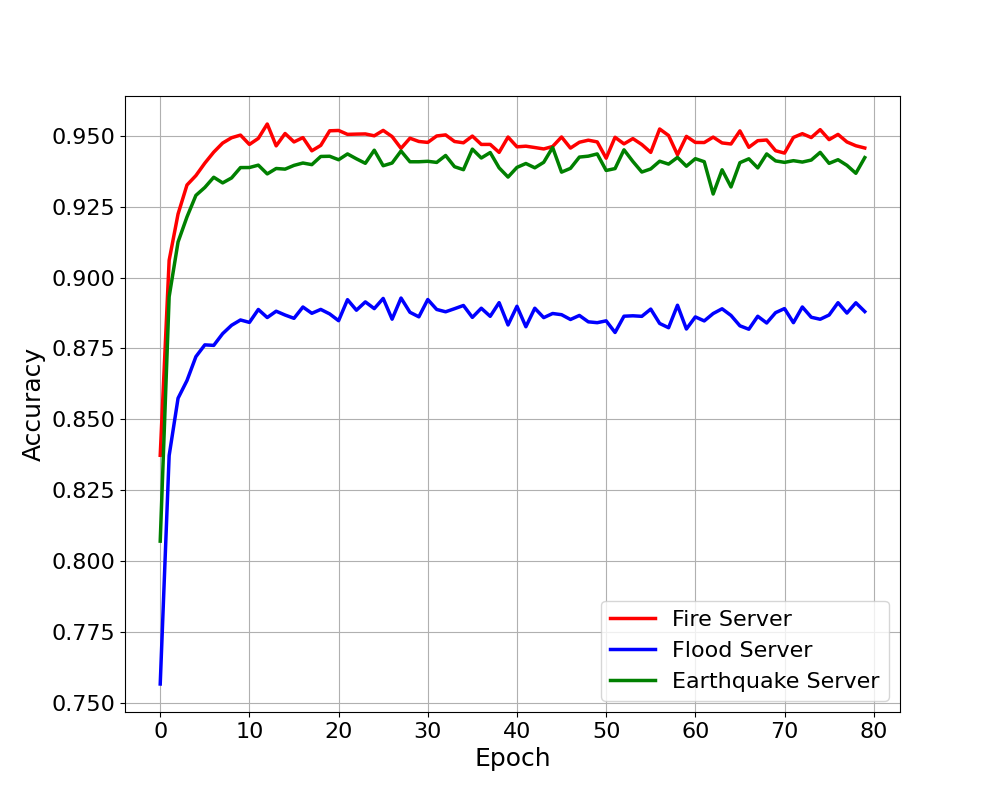
\includegraphics[width=0.75\textwidth]{figures/chapter2/User_Accuracies.png}
    \caption{Ακρίβεια κόμβων ανά εποχή}
    \label{fig1}
\end{figure}

\begin{figure}[H]
    \centering
    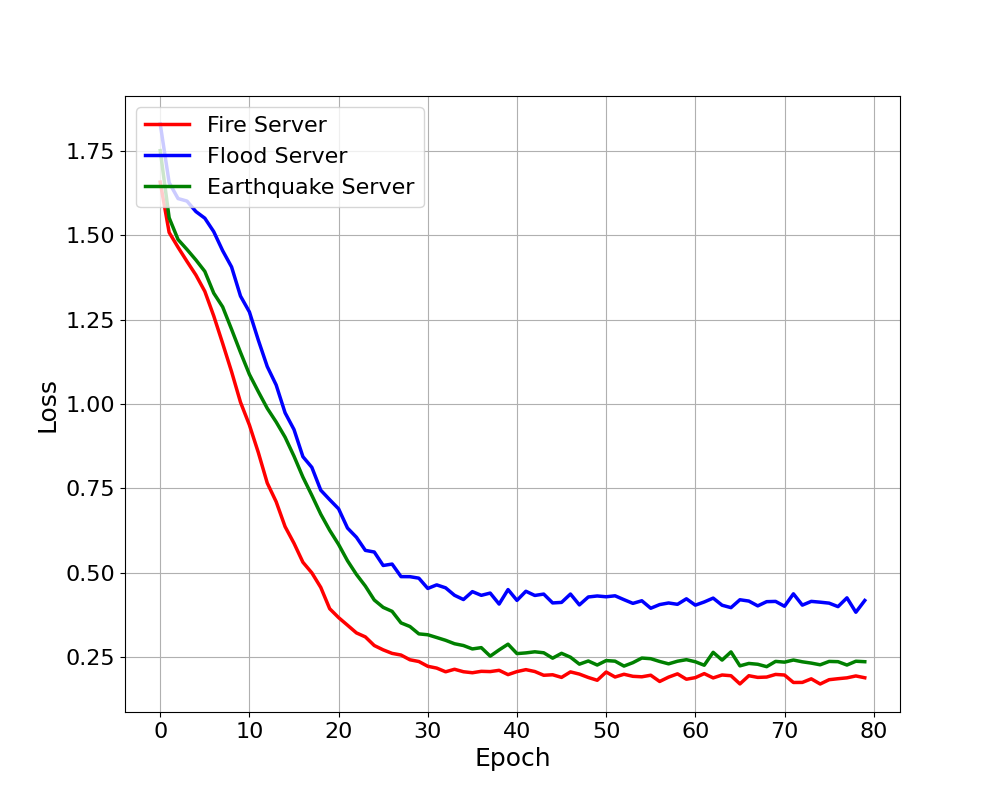
\includegraphics[width=0.75\textwidth]{figures/chapter2/User_Losses.png}
    \caption{Απώλεια κόμβων ανά εποχή}
    \label{fig2}
\end{figure}

\newpage

Όπως φαίνεται στα διαγράμματα \ref{fig1} και \ref{fig2} οι κόμβοι μας ξεκινούν την εκμάθηση και σταδιακά αφομοιώνουν την πληροφορία του παγκόσμιου μοντέλου, μαθαίνοντας και από τους υπόλοιπους κόμβους. Έτσι, η μέση ακρίβεια των κόμβων αυξάνεται σταδιακά, ενόσω κάθε κόμβος επεξεργάζεται ξανά τα δικά του δεδομένα σε συνδυασμό με την πληροφορία που δέχεται από τον εξυπηρετητή του, ενώ η απώλεια αντίστοιχα μειώνεται. Βλέπουμε πως μετά από περίπου 20 εποχές - επαναλήψεις αρχίζουν και οι δύο ποσότητες να σταθεροποιούνται καταλήγοντας σε σύγκλιση.

Αντίστοιχη συμπεριφορά παρατηρούμε στα διαγράμματα για τους Εξυπηρετητές. Η εξέταση της απόδοσης των εξυπηρετητών κατά τις εποχές παρουσιάζει μια συνεπή τάση, με τον Εξυπηρετητή Πυρκαγιάς να επιτυγχάνει σταθερά τη μεγαλύτερη ακρίβεια, ακολουθούμενος από τους Εξυπηρετητές Σεισμών και Πλημμυρών (\ref{fig3}), δεδομένου ότι ο Εξυπηρετητής Πυρκαγιάς διαθέτει μεγαλύτερο σύνολο δεδομένων και, κατά συνέπεια, επιδεικνύει ανώτερη απόδοση. Ωστόσο, μια ενδιαφέρουσα απόκλιση παρατηρείται στον Εξυπηρετητή Πλημμυρών, ο οποίος, παρά το γεγονός ότι διαθέτει μεγαλύτερο σύνολο δεδομένων σε σύγκριση με τον Εξυπηρετητή Σεισμών, παρουσιάζει χαμηλότερη απόδοση (\ref{fig3} – \ref{fig4}). Αυτή η ανωμαλία προκύπτει από τη συμπερίληψη εικόνων με περιεχόμενο νερού στα ουδέτερα σύνολα δεδομένων που μοιράζονται οι Εξυπηρετητές. Αυτές οι εικόνες εισάγουν σύγχυση στη διαδικασία εκπαίδευσης του Εξυπηρετητή Πλημμυρών, επηρεάζοντας τελικά αρνητικά την απόδοσή του. Όπως αναφέρουν και οι Barry et al. (\lcite{barry2023impact}) η ποιότητα των δεδομένων και ο θόρυβος μπορούν να επηρεάσουν σημαντικά την απόδοση του μοντέλου. Ειδικότερα αν οι καλοί κόμβοι του Εξυπηρετητή Πλημμυρών διαθέτουν παρεμφερείς εικόνες με αυτές του Ουδέτερου Συνόλου Δεδομένων η εκμάθηση γίνεται πολύ δύσκολη αφού αυτοί οι κόμβοι έχουν τη μεγαλύτερη συμμετοχή στη διαδικασία.

\begin{figure}[ht]
    \centering
    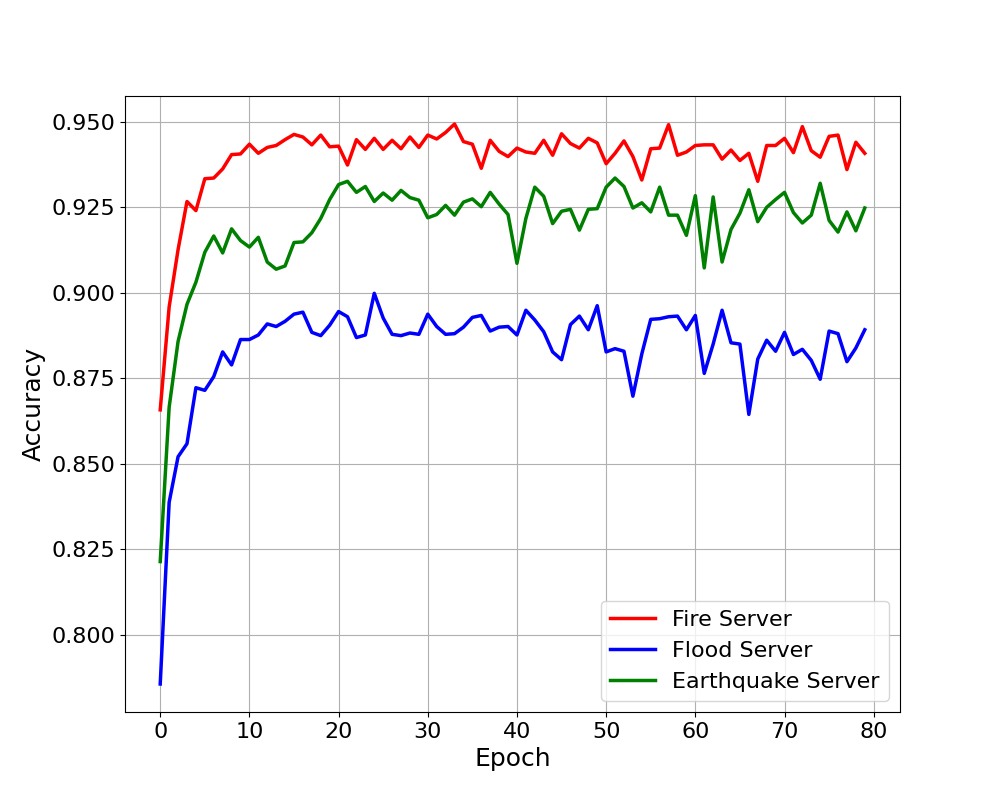
\includegraphics[width=0.75\textwidth]{figures/chapter2/Server_Accuracies.png}
    \caption{Ακρίβεια Εξυπηρετητών ανά εποχή}
    \label{fig3}
\end{figure}

\newpage

\begin{figure}[ht]
    \centering
    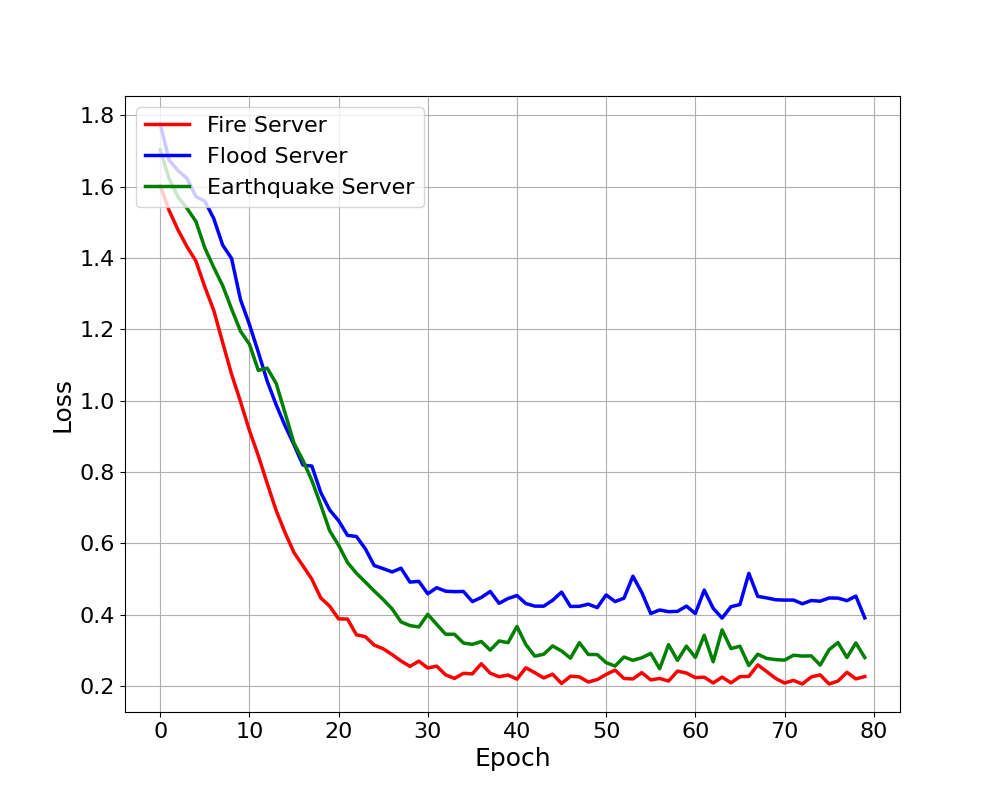
\includegraphics[width=0.75\textwidth]{figures/chapter2/Server_Losses.png}
    \caption{Απώλεια Εξυπηρετητών ανά εποχή}
    \label{fig4}
\end{figure}

Έτσι, ο Εξυπηρετητής Σεισμών, παρά το μικρότερο σύνολο δεδομένων, αποδίδει σχετικά καλύτερα από το αναμενόμενο, καταδεικνύοντας την πολύπλοκη σχέση μεταξύ μεγέθους συνόλου δεδομένων και απόδοσης. Επίσης, οι κόμβοι που σχετίζονται με τον Εξυπηρετητή Σεισμών επιτυγχάνουν σταθερά υψηλότερη τοπική ακρίβεια σε σύγκριση με τους κόμβους των Εξυπηρετητών Πυρκαγιάς και Πλημμυρών (\ref{fig1}), αποδεικνύοντας την αποτελεσματικότητα των αντίστοιχων συνόλων δεδομένων. Ωστόσο, η διαφορά στην απόδοση των κόμβων δεν αντικατοπτρίζει άμεσα την ιεραρχία που παρατηρείται στην απόδοση των Εξυπηρετητών. Αυτή η απόκλιση προκύπτει από τη δυσκολία της πραγματικής σύνθεσης των συνόλων των παραμέτρων στο παγκόσμιο μοντέλο, αλλά και από υπερπροσαρμογή των κόμβων του Εξυπηρετητή Σεισμών (διαφορά μεταξύ ακρίβειας εκπαίδευσης και ακρίβειας δοκιμών).

\newpage

\begin{figure}[H]
    \centering
    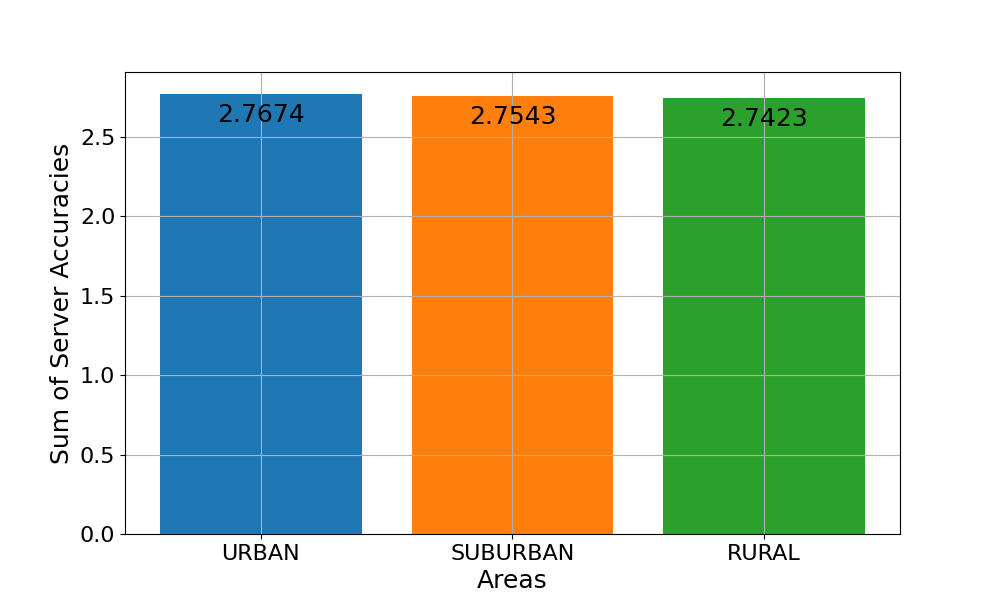
\includegraphics[width=\textwidth]{figures/chapter2/Sum_of_Accuracies_per_Area.png}
    \caption{Σενάριο Δημόσιας ασφάλειας σε διαφορετικές περιοχές (αστική, προαστική, αγροτική) - Ακρίβεια}
    \label{fig5}
\end{figure}

\begin{figure}[H]
    \centering
    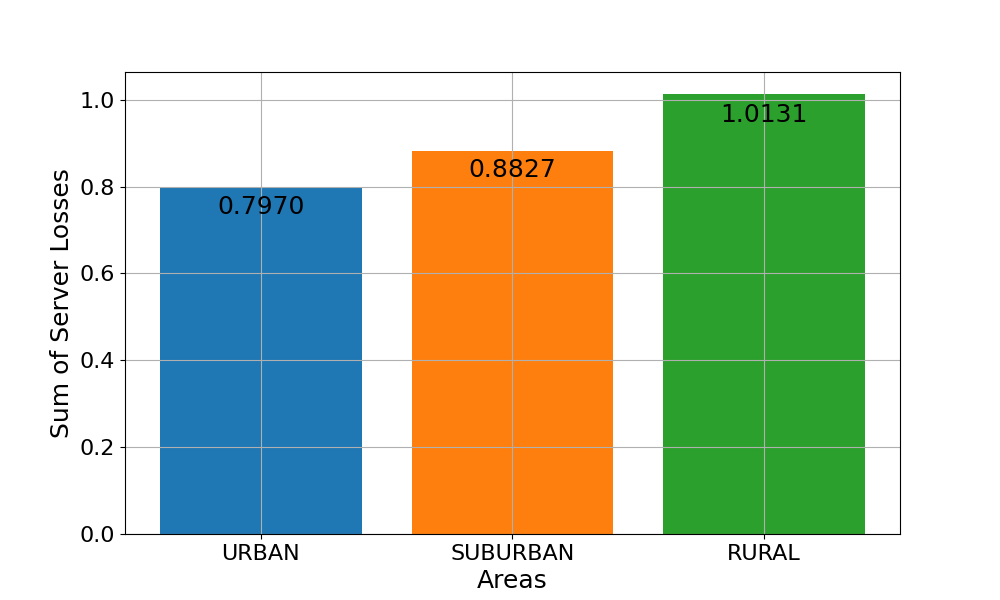
\includegraphics[width=\textwidth]{figures/chapter2/Sum_of_Losses_per_Area.png}
    \caption{Σενάριο Δημόσιας ασφάλειας σε διαφορετικές περιοχές (αστική, προαστική, αγροτική) - Απώλεια}
    \label{fig6}
\end{figure}

\newpage

Ο μηχανισμός αντιστοίχισης δοκιμάζεται σε ένα ρεαλιστικό σενάριο δημόσιας ασφάλειας σε αστικά, προαστιακά και αγροτικά περιβάλλοντα. Η \ref{fig5} παρουσιάζει το άθροισμα της ακρίβειας των εξυπηρετητών για τρία διακριτά σενάρια: Αστικό, Προαστιακό και Αγροτικό, καθένα από τα οποία χαρακτηρίζεται από διαφορετική σύνθεση κόμβων. Αντίστοιχα στο \ref{fig6} παρουσιάζει το άθροισμα της απώλειας των εξυπηρετητών στις τρεις αυτές περιοχές.

Σε κάθε σενάριο, οι κόμβοι κατηγοριοποιούνται είτε ως καλοί (κοντά στα Σημεία Ενδιαφέροντος) είτε ως κακοί (μακριά από τα Σημεία Ενδιαφέροντος, γεγονός που οδηγεί σε σύγχυση του αλγορίθμου και μειωμένη χρησιμότητα δεδομένων). Το όριο που διαχωρίζει τους καλούς από τους κακούς κόμβους διαφέρει μεταξύ των σεναρίων: Αστικό (30), Προαστιακό (21) και Αγροτικό (12), υποδεικνύοντας το σημείο πέρα από το οποίο οι κόμβοι θεωρούνται κακοί.

Τα αποτελέσματα αποκαλύπτουν ένα συνεπές πρότυπο για τα τρία σενάρια. Όσο οι κόμβοι μας είναι πιο απομακρυσμένοι από τα σημεία ενδιαφέροντος και άρα διαθέτουν λιγότερη πληροφορία, καθιστούν πιο δύσκολη την εκπαίδευση του κεντρικού μοντέλου. Για αυτό το λόγο, όπως φαίνεται, πετυχαίνουμε καλύτερη αθροιστική Ακρίβεια και μικρότερη σε μία Αστική Περιοχή απ' ότι σε μία Προαστιακή Περιοχή και μία Αγροτική Περιοχή. 

Από τη συμπεριφορά αυτή φαίνεται πώς η διαφοροποίηση ανά περιοχή με καλούς και κακούς κόμβους επηρεάζει την εκμάθηση των μοντέλων. Έχοντας κόμβους με λιγότερα δεδομένα - εικόνες να συμμετέχουν στην Ομοσπονδιακή Μάθηση, δυσκολεύει σε κάποιο βαθμό τη γενίκευση στο παγκόσμιο μοντέλο. Η αρνητική επίδραση αυτή καταπολεμάται από τον αλγόριθμό μας με τη χρήση βαρών συμμετοχής στην εκμάθηση, όπου ένας κακός κόμβος, με λιγότερα, άρα και πιο μη γενικευμένα δεδομένα, συμμετέχει λιγότερο σε σχέση με έναν κόμβο που διαθέτει περισσότερη πληροφορία, με αποτέλεσμα εν τέλει σε όλες τις περιοχές να πετυχαίνουμε πολύ καλά αποτελέσματα για τα παγκόσμια μοντέλα.

\chapter{Αντιστοίχιση με Αλγορίθμους Ενισχυτικής Μάθησης}

Στο δεύτερο, αυτό κομμάτι της διπλωματικής εργασίας, θα συγκρίνουμε τον Αλγόριθμο Θεωρίας Παιγνίων, που παρουσιάσαμε στο προηγούμενο κεφάλαιο, με άλλους αλγορίθμους που χρησιμοποιούνται σε παρόμοιες περιπτώσεις. Συγκεκριμένα θα μελετήσουμε την συμπεριφορά αλγορίθμων Μηχανικής Μάθησης - Ενισχυτικής Μάθησης, αλλά θα χρησιμοποιήσουμε και ως σημείο αναφοράς τον αλγόριθμο τυχαίας αντιστοίχισης, ώστε να αποφανθούμε για τα οφέλη που μας προσφέρουν οι υπόλοιποι αλγόριθμοι.

Η Ενισχυτική Μάθηση (Reinforcement Learning, RL) περιλαμβάνει μια ποικιλία αλγορίθμων που έχουν σχεδιαστεί για να μαθαίνουν τις βέλτιστες πολιτικές επιλογής ενεργειών μέσω αλληλεπιδράσεων με ένα περιβάλλον. Οι βασικές μέθοδοι βασισμένες σε τιμές περιλαμβάνουν τους αλγόριθμους Q-Learning και SARSA (State-Action-Reward-State-Action). Το Q-Learning είναι ένας εκτός πολιτικής αλγόριθμος που ενημερώνει επαναληπτικά τις τιμές Q για να εκτιμήσει την αναμενόμενη χρησιμότητα των ενεργειών σε δεδομένες καταστάσεις, ανεξάρτητα από τις ενέργειες του πράκτορα (ατόμου - κόμβου). Στοχεύει να μάθει την βέλτιστη πολιτική μεγιστοποιώντας τη συνολική ανταμοιβή με την πάροδο του χρόνου. Αντίθετα, το SARSA είναι ένας εντός πολιτικής αλγόριθμος που ενημερώνει τις τιμές Q βάσει των πραγματικών ενεργειών που λαμβάνονται από την πολιτική, αντί της μέγιστης δυνατής ενέργειας. Αυτό επιτρέπει στο SARSA να ενσωματώνει άμεσα τα αποτελέσματα της τρέχουσας πολιτικής του πράκτορα στη διαδικασία μάθησης. \lcite{reinforcement_overview_classification}

Τα Βαθειά Q-Δίκτυα (Deep Q-Networks - DQN) επεκτείνουν το Q-Learning ενσωματώνοντας βαθιά νευρωνικά δίκτυα, επιτρέποντας τη διαχείριση χώρων καταστάσεων υψηλής διάστασης. Τα Βαθειά Q-Δίκτυα χρησιμοποιούν αναπαραγωγή εμπειριών για να αποθηκεύουν και να επαναχρησιμοποιούν παλαιότερες εμπειρίες, βοηθώντας στη διακοπή της συσχέτισης μεταξύ διαδοχικών βημάτων μάθησης και βελτιώνοντας την αποδοτικότητα της εκπαίδευσης. Επιπλέον, τα Βαθειά Q-Δίκτυα χρησιμοποιούν ένα δίκτυο στόχου για να παρέχουν σταθερούς στόχους τιμών Q, μειώνοντας έτσι τα προβλήματα αστάθειας που προκύπτουν κατά την εκπαίδευση νευρωνικών δικτύων. \lcite{reinforcement_overview_classification}

Στην δική μας περίπτωση, οι τεχνικές Ενισχυτικής Μάθησης χρησιμοποιούνται όλο και περισσότερο στις λειτουργίες αντιστοίχισης σε διάφορους τομείς, όπως συστήματα συστάσεων, διαδικτυακή διαφήμιση και κατανομή πόρων. Σε αυτές τις εφαρμογές, οι αλγόριθμοι Ενισχυτικής Μάθησης, βελτιστοποιούν τη διαδικασία αντιστοίχισης μαθαίνοντας από τις αλληλεπιδράσεις με το περιβάλλον. Για παράδειγμα, στα συστήματα συστάσεων, οι πράκτορες Ενισχυτικής Μάθησης βελτιώνουν διαδοχικά τις προτάσεις τους λαμβάνοντας υπόψη την ανατροφοδότηση των κόμβων και ενημερώνοντας τις πολιτικές τους για τη μεγιστοποίηση της μακροπρόθεσμης εμπλοκής και ικανοποίησης των κόμβων. \lcite{Afsar2022}

Σε αντίστοιχη περίπτωση, μπορούμε να χρησιμοποιήσουμε τέτοιους αλγορίθμους για την αντιστοίχιση των κόμβων μας με τους εξυπηρετητές. Μέσω της Ενισχυτικής Μάθησης, οι κόμβοι λαμβάνουν αμοιβές ανάλογα με την ενέργεια που επιλέγουν κάθε φορά και έπειτα από συγκεκριμένο αριθμό επαναλήψεων, ο κάθε κόμβος επιλέγει την βέλτιστη ενέργεια με βάση τις αμοιβές που έχει συλλέξει. 

\section{Περιγραφή Αλγορίθμων Ενισχυτικής Μάθησης}

Για την εξερεύνηση και επιλογή ενεργειών από τους κόμβους θα χρησιμοποιήσουμε την αλγοριθμική τεχνική Ανώτατου Ορίου Εμπιστοσύνης (Upper Confidence Bound - UCB). Ο αλγόριθμος Ανώτατου Ορίου Αυτοπεποίθησης είναι μια στρατηγική που χρησιμοποιείται στη ενισχυτική μάθηση και στα προβλήματα πολλαπλών ένοπλων ληστών (multi-armed bandit) για να εξισορροπήσει αποτελεσματικά την εξερεύνηση και την εκμετάλλευση. Σε αντίθεση με απλές μεθόδους όπως ο αλγόριθμος ε-άπληστος (ε-greedy), ο Ανώτατου Ορίου Αυτοπεποίθησης επιλέγει ενέργειες με βάση τόσο τις εκτιμώμενες ανταμοιβές όσο και την αβεβαιότητα σε αυτές τις εκτιμήσεις. Δίνοντας προτεραιότητα σε ενέργειες με μεγαλύτερη αβεβαιότητα, ο Ανώτατου Ορίου Αυτοπεποίθησης εξερευνά συστηματικά λιγότερο δοκιμασμένες επιλογές, διασφαλίζοντας ότι ο αλγόριθμος συγκεντρώνει επαρκείς πληροφορίες για όλες τις πιθανές ενέργειες. Αυτή η προσέγγιση βοηθά στην πιο αξιόπιστη αναγνώριση της βέλτιστης ενέργειας με την πάροδο του χρόνου. Η μεθοδική μέθοδος του Ανώτατου Ορίου Αυτοπεποίθησης για την εξισορρόπηση της εξερεύνησης και της εκμετάλλευσης τον καθιστά ιδιαίτερα χρήσιμο σε σενάρια όπου η κατανόηση των υποκείμενων κατανομών ανταμοιβής είναι κρίσιμη για την μακροπρόθεσμη επιτυχία. \lcite{sutton2018ucb}

Στην περίπτωσή μας, ακολουθούμε την εξής διαδικασία: Αρχικά, κάθε κόμβος δεν ανήκει σε κανέναν εξυπηρετητή. Σε κάθε επανάληψη, κάθε κόμβος συλλέγει τις ενέργειες που μπορεί να επιλέξει να εκτελέσει. Στην συνέχεια εφαρμόζει τον κανόνα επιλογής ενέργειας του Αλγορίθμου Ανώτατου Ορίου Αυτοπεποίθησης για να επιλέξει την βέλτιστη ενέργεια σύμφωνα με τα μέχρι τώρα δεδομένα του (προφανώς αρχικά δεν έχει λάβει κάποια ανατροφοδότηση από το περιβάλλον του). Ο κανόνας επιλογής ενέργειας του αλγορίθμου επιλέγει την ενέργεια που μεγιστοποιεί το ανώτερο όριο εμπιστοσύνης της εκτιμώμενης ανταμοιβής. Το ανώτερο όριο εμπιστοσύνης υπολογίζεται ως:

\begin{equation}
    a_t = \arg \max_a \left( \hat{Q}(a) + c \sqrt{\frac{\ln t}{N(a)}} \right)
    \label{eq16}
\end{equation}

όπου:

\begin{itemize}
  \item $\hat{Q}(a)$ είναι η εκτιμώμενη ανταμοιβή για την ενέργεια $a$.
  \item $t$ είναι ο συνολικός αριθμός φορών που έχει επιλεχθεί μια ενέργεια.
  \item $N(a)$ είναι ο αριθμός φορών που έχει επιλεχθεί η ενέργεια $a$.
  \item $c$ είναι μια σταθερά που εξισορροπεί την εξερεύνηση και την εκμετάλλευση.
\end{itemize}

Ο όρος \(\sqrt{\frac{\ln t}{N(a)}}\) αντιπροσωπεύει την αβεβαιότητα ή το διάστημα εμπιστοσύνης για την εκτιμώμενη ανταμοιβή. Οι ενέργειες με λιγότερες επιλογές ($N(a)$) θα έχουν μεγαλύτερη αβεβαιότητα, ενθαρρύνοντας την εξερεύνηση.

Αφού επιλεγεί η βέλτιστη ενέργεια, ο κόμβος την εκτελεί και λαμβάνει την αντίστοιχη ανταμοιβή - ανατροφοδότηση, από το δίκτυο. Επιπλέον, ανανεώνει την εκτιμώμενη ανταμοιβή του για την ενέργεια \textbf{α} ως:

\begin{equation}
    \hat{Q}(a) = \hat{Q}(a) + \gamma (r - \hat{Q}(a))
    \label{eq17}
\end{equation}

\noindent
όπου \textbf{r} είναι η ανταμοιβή-ανατροφοδότηση που λαμβάνει από το δίκτυο και \textbf{γ} ο όρος που καθορίζει πόσο σημαντικές είναι για την εκτιμώμενη ανταμοιβή οι μελλοντικές ανταμοιβές που λαμβάνει.

Οι υπόλοιποι κόμβους ακολουθούν την ίδια διαδικασία, αφού όμως έχει εκτελεστεί η ενέργεια του πρώτου κόμβου, με αποτέλεσμα να έχει αλλάξει το οικοσύστημα. Η διαδικασία αυτή επαναλαμβάνεται μέχρι να πετύχουμε σύγκλιση του αλγορίθμου. Η σύγκλιση εξασφαλίζεται όταν η διαφορά των πινάκων Q(a) σε δύο διαδοχικές επαναλήψεις είναι για κάθε ενέργεια κάτω από μια συγκεκριμένη τιμή ανοχής (tolerance). Όταν επιτευχθεί η σύγκλιση, κάθε κόμβος, με βάση τις αμοιβές που έχει συλλέξει, αποφασίζει για την ενέργεια την οποία θα λάβει τελικά.

Στην εργασία αυτή θα μελετήσουμε δύο εκδοχές του αλγορίθμου, οι οποίες χρησιμοποιούν διαφορετικές εκδοχές συνάρτησης ανταμοιβής για κάθε ενέργεια. Η πρώτη βασίζεται στην εστίαση στον κόμβου, δηλαδή ως ανταμοιβή για μια ενέργεια δίνεται η χρησιμότητα του κόμβου (Εξίσωση \ref{eq7}) έπειτα από την επιλογή της ενέργειας:

\begin{equation}
    reward(a) = U_{n,s}
    \label{eq18}
\end{equation}

\noindent
όπου $s$ είναι ο εξυπηρετητής που επιλέγεται από την ενέργεια του κόμβου $n$ που θεωρήθηκε βέλτιστη.

Η δεύτερη εκδοχή, εστιάζει στην προτίμηση των εξυπηρετητών και άρα αυτή τη φορά ορίζουμε ως ανταμοιβή την μέση χρησιμότητα ανά κόμβου που βιώνει ο εξυπηρετητής (Εξίσωση \ref{eq8}):

\begin{equation}
    reward(a) = \frac{U_s(P_s,P_{-s})}{N_s}
    \label{eq19}
\end{equation}

\noindent
όπου $s$ είναι ο εξυπηρετητής που επιλέγεται από την ενέργεια του κόμβου $n$ που θεωρήθηκε βέλτιστη και $N_s$ το πλήθος του συνασπισμού του $s$.

\newpage

\begin{algorithm}[h]
\caption{Αλγόριθμος Αντιστοίχισης με Ενισχυτική Μάθηση} \label{algorithm 3}
\begin{algorithmic}[1]
\STATE \textbf{\underline{Είσοδος:}} ${L_n, a_n, q_n, D_n, f_n, \mathbf{w}_n}{\forall n\in \mathcal{N}}, {L_k}{\forall k \in \mathcal{K}}, \alpha,\beta,\gamma$,

\STATE \textbf{\underline{Έξοδος:}} \text{Αποτελέσματα Αντιστοίχισης} $M$
\STATE \textbf{\underline{Αρχικοποίηση:}} $cumulative\_reward = 0$, $N_t = 0$, $Q_n = 0 \>\> \forall$ πιθανή ενέργεια και $\forall n \in N$
\WHILE{not convergence}
\FOR{$n \in \mathcal{N}$}
\STATE Ο κόμβος $n$ επιλέγει την βέλτιστη ενέργεια με βάση την Εξίσωση \ref{eq16}.
\STATE Εκτελεί την ενέργεια και λαμβάνει την αντίστοιχη ανταμοιβή με βάσει τις εξισώσεις \ref{eq18} και \ref{eq19}.
\STATE Τέλος ανανεώνει τα: $cumulative\_reward(n,a) += reward$, $Nt(n,a) += 1$ και $Qn$ με βάση την εξίσωση \ref{eq17}
\ENDFOR
\ENDWHILE
\FOR{$n \in \mathcal{N}$}
\STATE Ο κόμβος $n$ επιλέγει την βέλτιστη ενέργεια με βάση το μεγαλύτερο cumulative reward που έχει συλλέξει για κάθε ενέργεια.
\ENDFOR
\end{algorithmic}
\end{algorithm}
\vspace{-7pt}

Τέλος, όπως αναφέραμε, ως σημείο αναφοράς θα χρησιμοποιήθεί ο Αλγόριθμος Τυχαίας Αντιστοίχισης, σύμφωνα με τον οποίο κάθε κόμβος αντιστοιχίζεται τυχαία σε κάποιον εξυπηρετητής, τηρώντας προφανώς το όριο $Ns_{max}$ του κάθε εξυπηρετητή.

\begin{algorithm}[h]
\caption{Αλγόριθμος Τυχαίας Αντιστοίχισης} \label{algorithm 4}
\begin{algorithmic}[1]
\STATE \textbf{\underline{Είσοδος:}} ${L_n, a_n, q_n, D_n, f_n, \mathbf{w}_n}{\forall n\in \mathcal{N}}, {L_k}{\forall k \in \mathcal{K}}, \alpha,\beta,\gamma$,

\STATE \textbf{\underline{Έξοδος:}} \text{Αποτελέσματα Αντιστοίχισης} $M$

\FOR{$n \in \mathcal{N}$}
\STATE Ο κόμβος $n$ επιλέγει τυχαία έναν εξυπηρετητή εφ'όσον αυτός διαθέτει χώρο στον συνασπισμό του.
\ENDFOR
\end{algorithmic}
\end{algorithm}
\vspace{-7pt}

\section{Υλοποίηση}

\textbf{Αλλαγή Οικοσυστήματος κόμβων - Εξυπηρετητών:} Στο συγκεκριμένο κεφάλαιο, για να εξεταστούν σε μεγαλύτερο βάθος οι επιδόσεις των διαφορετικών αλγορίθμων για την σύγκρισή τους, αλλάζουμε λίγο τον τρόπο με τον οποίο τοποθετούμε πάνω στον "χάρτη" τους κόμβους μας και τα κρίσιμα σημεία. Πιο συγκεκριμένα, ορίζουμε την ελάχιστη απόσταση μεταξύ δύο σημείων σε 0.4 και άρα πλέον, για μεγαλύτερα Ν είναι πιο πιθανό οι πιο απομακρισμένοι κόμβοι να προσφέρουν καλύτερη χρησιμότητα για άλλους εξυπηρετητές, απ' ότι για αυτόν του κρίσιμου σημείου γύρω από το οποίο τοποθετήθηκαν αρχικά. Οι απομακρισμένοι λοιπόν κόμβοι, θα μας δώσουν μια πιο ξεκάθαρη εικόνα για το ποιος αλγόριθμος λειτουργεί καλύτερα και σε πιο δύσκολες και όχι απαραίτητα προφανείς καταστάσεις. Επιπλέον, για να δώσουμε επιπλέον διαφοροποίηση και ισχύ στους εξυπηρετητές, κάθε εξυπηρετητής τώρα διαθέτει χρηματικούς πόρους μεταξύ $\ceil*{\frac{N}{3}}$ και $\ceil*{\frac{N}{2}}$. Συνεπώς, όντας κάποιοι εξυπηρετητές πιο ισχυροί, θα έχουν την δυνατότητα να προσελκύσουν πιο εύκολα κόμβους σε αυτούς και άρα θα είναι πιο πιθανό κάποιοι απομακρισμένοι κόμβοι να τους προτιμήσουν. Επιπλέον, δεν ασχολούμαστε πλέον με διαφορετικές περιοχές κόμβων (Αστική, Προαστιακή, Αγροτική), απλά τοποθετούμε κόμβους γύρω από τα κρίσιμα σημεία μας, με στόχο να μελετήσουμε την συμπεριφορά των διαφορετικών αλγορίθμων αντιστοίχισης.

Για την ορθή σύγκριση των αλγορίθμων, φροντίζουμε και οι τρεις να δέχονται ως είσοδο τους ίδιους κόμβους, δηλαδή να μην δημιουργούμε ξανά νέα αντικείμενα κόμβων. Αυτό μας εξασφαλίζει αντίστοιχα ότι οι σημασίες των κόμβων μας για κάθε εξυπηρετητή παραμένουν οι ίδιες και άρα οι αλγόριθμοί μας ανταγωνίζονται στο ίδιο περιβάλλον. Αντίστοιχα, όπως και στο προηγούμενο κεφάλαιο, φροντίζουμε, με ντετερμινιστικά τυχαίο τρόπο, οι κόμβοι μας να λάβουν τα ίδια δεδομένα-φωτογραφίες σε κάθε περίπτωση, ώστε κατά την εκπαίδευση του συστήματος που παράγει κάθε αλγόριθμος, να πάρουμε αντιπροσωπευτικά αποτελέσματα για την σύγκρισή τους. 

\section{Σύγκριση - Αποτελέσματα}

Σύμφωνα με τα αποτελέσματά μας, ο αλγόριθμος Θεωρίας Παιγνίων αποδίδει καλύτερα στις περισσότερες περιπτώσεις. Πετυχαίνει βέλτιστη αντιστοίχιση στα περισσότερες διαμορφώσεις του περιβάλλοντος μας (διαφορετικά πλήθη κόμβων), ενώ οι αλγόριθμοι Μηχανικής Μάθησης φαίνεται να κάνουν υποβέλτιστες αντιστοιχίσεις, κάνοντας λάθη, ειδικά όταν ο αριθμός των κόμβων μεγαλώνει και έχουμε και πιο απομακρισμένους κόμβους. Ως βασικό σημείο αναφοράς έχουμε την επίδοση του τυχαίου αλγορίθμου αντιστοίχισης, ο οποίος εκτελείται ταχύτατα.  Πιο συγκεκριμένα παίρνουμε τα εξής διαγράμματα:

\begin{figure}[H]
    \centering
    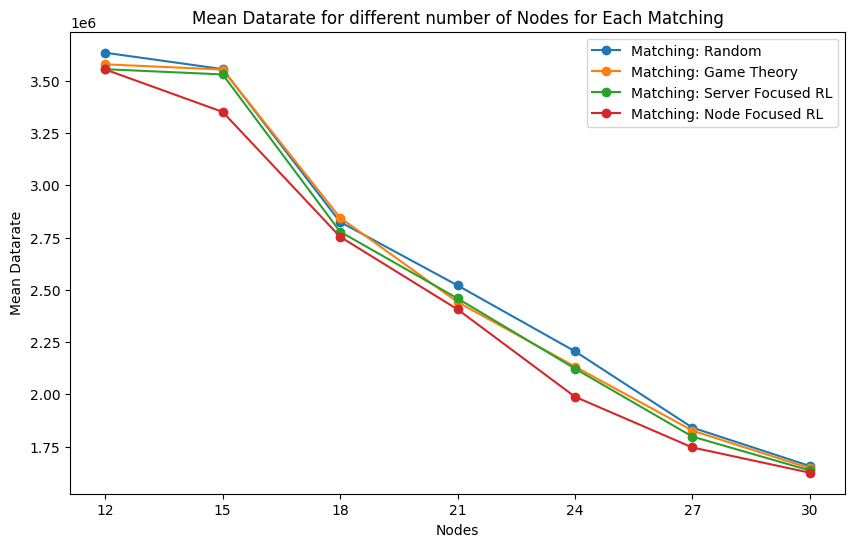
\includegraphics[width=\textwidth]{figures/chapter3/Mean_Datarate_vs_Nodes.png}
    \caption{Μέση ροή δεδομένων ανά αριθμό κόμβων ανά αλγόριθμο αντιστοίχισης}
    \label{fig7}
\end{figure}

Όπως φαίνεται στο \ref{fig7} οι αλγόριθμοί μας παρουσιάζουν αντίστοιχες μέσες ροές δεδομένων για τους κόμβους τους. Παραδόξως ο αλγόριθμος Τυχαίας Αντιστοίχισης φαίνεται να έχει την καλύτερη απόδοση κατά μέσο όρο. Αυτό συμβαίνει επειδή δεν λαμβάνει υπόψη του τις άλλες παραμέτρους και άρα είναι πιθανό να κάνει μια "πιο δίκαιη" κατανομή των κόμβων στους εξυπηρετητές, όσον αφορά την ροή δεδομένων. Αντίθετα οι άλλοι αλγόριθμοι κοιτούν να αυξήσουν την χρησιμότητα του συστήματος η οποία διαθέτει και άλλες παραμέτρους. Παρατηρούμε πως όσο αυξάνεται ο αριθμός των κόμβων, η ροή δεδομένων μειώνεται, αφού περισσότεροι κόμβοι ανταγωνίζονται για τους διαθέσιμους πόρους κάθε εξυπηρετητή (εύρος ζώνης). Συνεπώς, όσο περισσότερους κόμβους έχουμε στο σύστημά μας τόσο λιγότερα δεδομένα μπορούν να στείλουν ταυτόχρονα στον κοινό εξυπηρετητή τους.

\begin{figure}[ht]
    \centering
    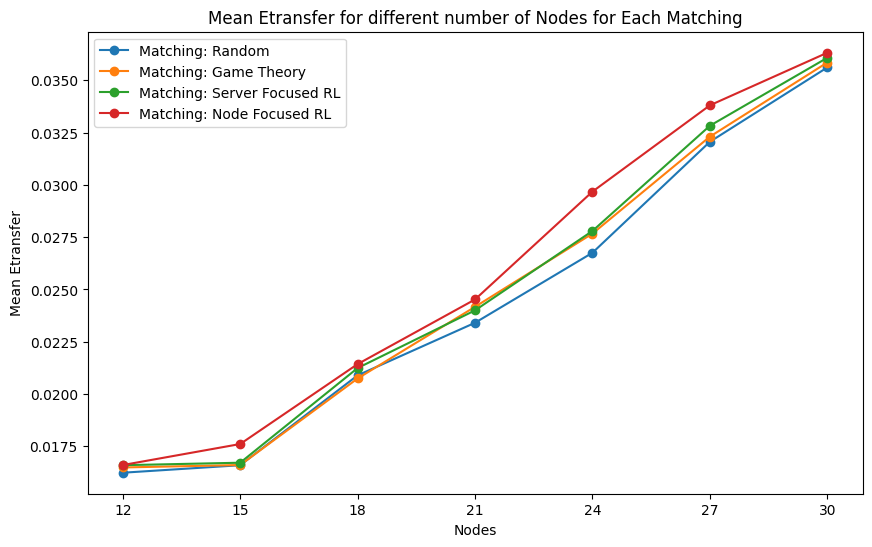
\includegraphics[width=\textwidth]{figures/chapter3/Mean_Etransfer_vs_Nodes.png}
    \caption{Μέση ενέργεια μετάδοσης ανά αριθμό κόμβων ανά αλγόριθμο αντιστοίχισης}
    \label{fig8}
\end{figure}

Όπως είναι εμφανές στο διάγραμμα \ref{fig8} και αναφέραμε και για την ροή δεδομένων, όσο περισσότερους κόμβους έχουμε, αυτοί ανταγωνίζονται για περισσότερους πόρους και άρα η μέση ενέργεια μετάδοσης αυξάνεται. Όπως, βλέπουμε αντίστοιχα, ο αλγόριθμος Τυχαίας Αντιστοίχισης κρατά την ενέργεια μετάδοσης χαμηλότερα απ' όλους, αφού δεν παίρνει υπόψη του την συνάρτηση χρησιμότητας, η οποία εξετάζει και άλλες παραμέτρους. Την δεύτερη καλύτερη επίδοση έχει ο αλγόριθμος Θεωρίας Παιγνίων, ο οποίος υπερέχει των δύο αλγορίθμων Ενισχυτικής Μάθησης.

Όσον αφορά την ποιότητα δεδομένων, βλέπουμε στο \ref{fig52} πως και πάλι ο αλγόριθμος Θεωρίας Παιγνίων πετυχαίνει το καλύτερο αποτέλεσμα, με σταθερά καλύτερη ποιότητα δεδομένων. Όσο εισέρχονται κόμβοι στο σύστημά μας η μέση ποιότητα μειώνεται, αφού οι νέοι κόμβοι τοποθετούνται όλο και πιο μακριά, με αποτέλεσμα να έχουν και λιγότερα δεδομένα. Η ποιότητα δεδομένων είναι ένα πολύ σημαντικό μέγεθος, αφού επηρεάζει άμεσα την εκπαίδευση του μοντέλου Ομοσπονδιακής Μάθησης. 

\newpage

\begin{figure}[ht]
    \centering
    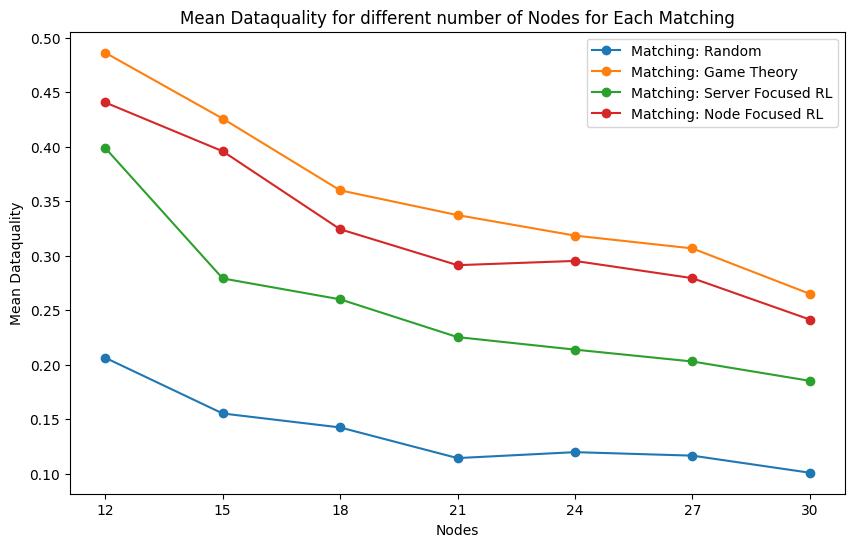
\includegraphics[width=\textwidth]{figures/chapter3/Mean_Dataquality_vs_Nodes.png}
    \caption{Μέση ποιότητα δεδομένων ανά αριθμό κόμβων ανά αλγόριθμο αντιστοίχισης}
    \label{fig52}
\end{figure}

\begin{figure}[H]
    \centering
    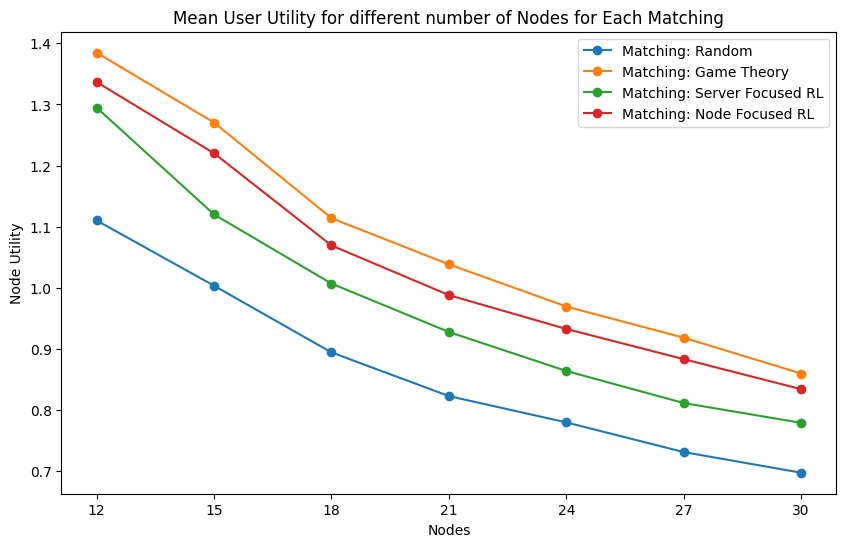
\includegraphics[width=\textwidth]{figures/chapter3/Mean_User_Utility_vs_Nodes.png}
    \caption{Μέση χρησιμότητα κόμβων ανά αριθμό κόμβων ανά αλγόριθμο αντιστοίχισης}
    \label{fig9}
\end{figure}

\newpage

Αντίστοιχα στο διάγραμμα \ref{fig9}, παίρνοντας μετρήσεις για την μέση χρησιμότητα των κόμβων, αυτή σταδιακά μειώνεται όσο ο αριθμός των κόμβων αυξάνεται, επειδή και πάλι έχουμε ανταγωνισμό μεταξύ τους. Σε αυτή τη μέτρηση, ο αλγόριθμος Θεωρίας Παιγνίων πετυχαίνει το καλύτερο αποτέλεσμα, ακολουθούμενος από τους αλγορίθμους Ενισχυτικής Μάθησης και τέλος από την Τυχαία Αντιστοίχιση.

\begin{figure}[H]
    \centering
    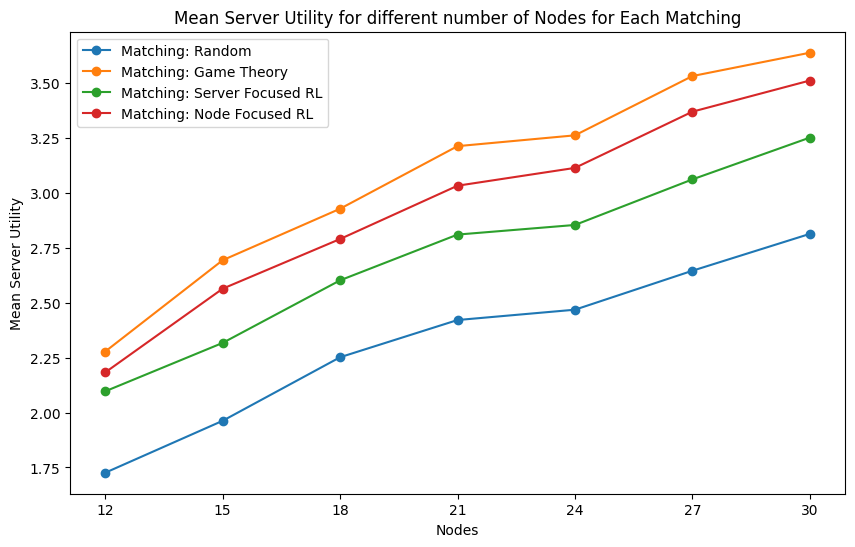
\includegraphics[width=\textwidth]{figures/chapter3/Mean_Server_Utility_vs_Nodes.png}
    \caption{Μέση χρησιμότητα εξυπηρετητών ανά αριθμό κόμβων ανά αλγόριθμο αντιστοίχισης}
    \label{fig10}
\end{figure}

Αντίθετα στο διάγραμμα \ref{fig10}, η μέση χρησιμότητα των εξυπηρετητών αυξάνεται όσο περισσότεροι κόμβοι εισέρχονται στο σύστημά μας, αφού κάθε συμμαχία διαθέτει περισσότερους κόμβους και άρα περισσότερη πληροφορία. Ο αλγόριθμος Θεωρίας Παιγνίων και εδώ φαίνεται να κάνει τις καλύτερες αντιστοιχίσεις.

Προφανώς όσο περισσότερους κόμβους έχουμε στο σύστημά μας τόσο πιο δύσκολο θα είναι για τους αλγορίθμους μας να κάνουν την αντιστοίχισή τους στους εξυπηρετητές. Βλέποντας τα δεδομένα στο διάγραμμα \ref{fig11}, ο πιο γρήγορος αλγόριθμος είναι ο αλγόριθμος Τυχαίας Αντιστοίχισης, αφού είναι και ο πιο απλός. Από τους υπόλοιπους, ο αλγόριθμος Θεωρίας Παιγνίων επιτυγχάνει την πιο αργή αντιστοίχιση, ακολουθούμενος από τους Αλγορίθμους Ενισχυτικής Μάθησης. Είναι αξιοσημείωτο πως ο αλγόριθμος Ενισχυτικής Μάθησης με βάση την χρησιμότητα κόμβων, πετυχαίνει ταχύτατες αντιστοιχίσεις, σε χρόνο πολύ κοντά σε αυτόν της Τυχαίας Αντιστοίχισης.

\newpage

\begin{figure}[ht]
    \centering
    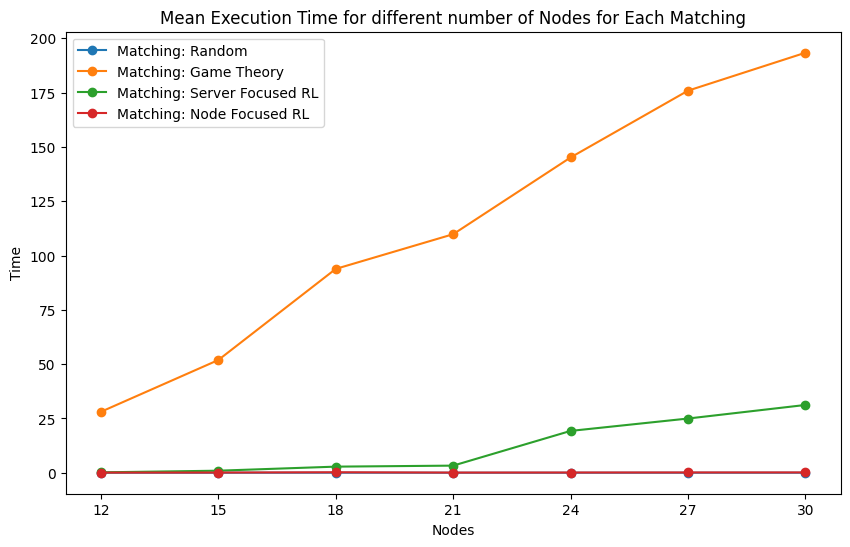
\includegraphics[width=0.9\textwidth]{figures/chapter3/Time_vs_Nodes.png}
    \caption{Μέσος χρόνος εκτέλεσης ανά αριθμό κόμβων ανά αλγόριθμο αντιστοίχισης}
    \label{fig11}
\end{figure}

Παρακάτω παρουσιάζουμε τις συνολικές διαφορές σε όλα τα πειράματα που έγιναν μεταξύ των διάφορων αλγορίθμων.

Όπως φαίνεται στο διάγραμμα \ref*{fig12} η Τυχαία Αντιστοίχιση πετυχαίνει κατά μέσο όρο το καλύτερο αποτέλεσμα όσον αφορά τη ροή δεδομένων από τους κόμβους στους εξυπηρετητές. Ελάχιστα χειρότερα αποτελέσματα πετυχαίνουν οι υπόλοιποι αλγόριθμοι με τον αλγόριθμο Θεωρίας Παιγνίων να ξεχωρίζει από αυτούς.

\begin{figure}[H]
    \centering
    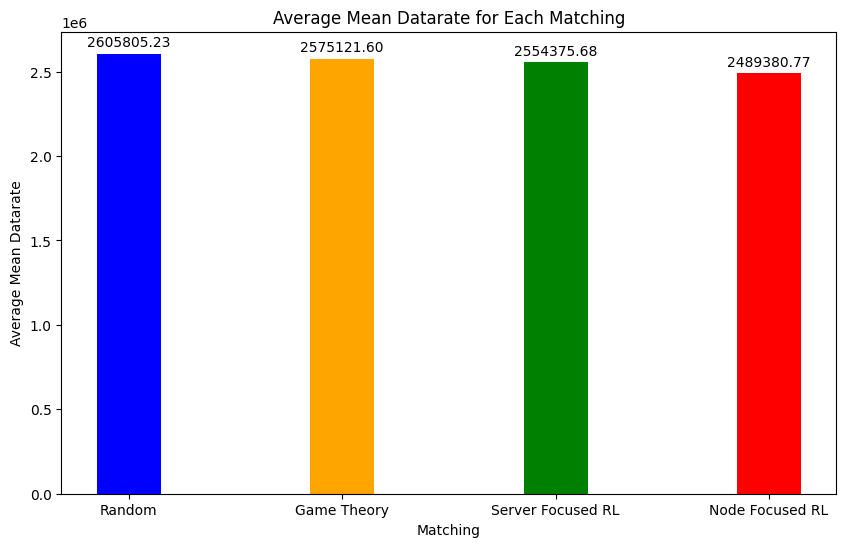
\includegraphics[width=0.9\textwidth]{figures/chapter3/Average_Mean_Datarate.png}
    \caption{Μέση ροή δεδομένων ανά αλγόριθμο αντιστοίχισης}
    \label{fig12}
\end{figure}

\newpage

\begin{figure}[H]
    \centering
    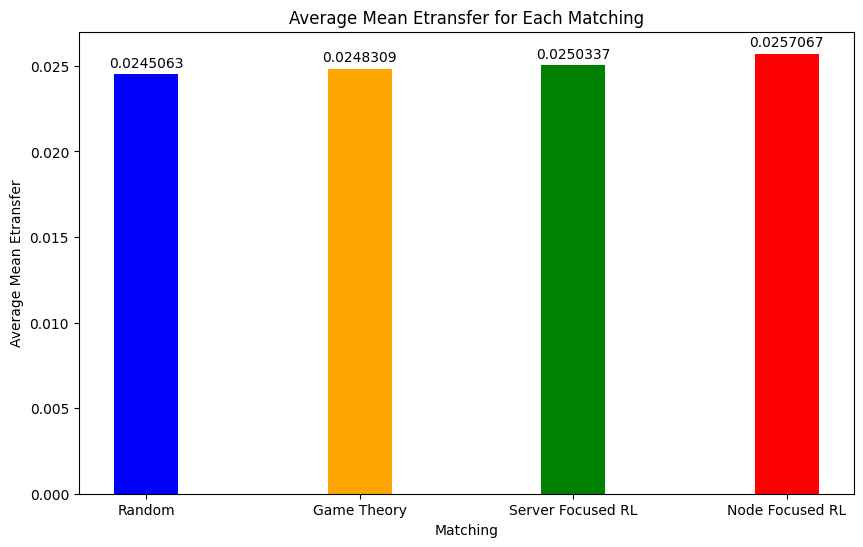
\includegraphics[width=0.9\textwidth]{figures/chapter3/Average_Mean_Etransfer.png}
    \caption{Μέση ενέργεια μετάδοσης ανά αλγόριθμο αντιστοίχισης}
    \label{fig13}
\end{figure}

Στο διάγραμμα \ref*{fig13} βλέπουμε τις επιδόσεις των αλγορίθμων αναφορικά με τη μέση ενέργεια μετάδοσης που απαιτείται για την αποστολή των παραμέτρων των τοπικών μοντέλων στους εξυπηρετητές. Η Τυχαία Αντιστοίχιση, έχοντας εξασφαλίσει την ταχύτερη κατά μέσο όρο ροή δεδομένων, πετυχαίνει την μικρότερη ενέργεια μετάδοσης, με τον αλγόριθμο Θεωρίας Παιγνίων να ακολουθεί και τέλος τους αλγορίθμους Ενισχυτικής Μάθησης. Παρ' όλα ταύτα, όλοι οι αλγόριθμοι είναι πολύ κοντά σε τιμές.

\begin{figure}[H]
    \centering
    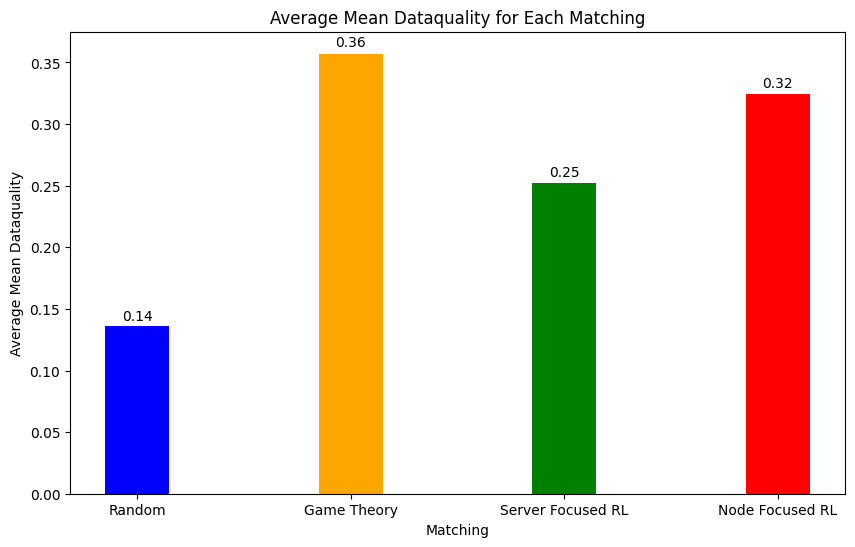
\includegraphics[width=0.9\textwidth]{figures/chapter3/Average_Mean_Dataquality.png}
    \caption{Μέση ποιότητα δεδομένων ανά αλγόριθμο αντιστοίχισης}
    \label{fig53}
\end{figure}

\newpage

Όσον αφορά την ποιότητα δεδομένων, μπορούμε να δούμε το καθαρό μειονέκτημα της Τυχαίας Αντιστοίχισης, η οποία πετυχαίνει πολύ χειρότερα αποτελέσματα από τους υπόλοιπους αλγορίθμους. Ο αλγόριθμος Θεωρίας Παιγνίων υπερέχει των υπολοίπων, ακολουθούμενος από τον αλγόριθμο Ενισχυτικής Μάθησης ως προς τη χρησιμότητα κόμβων.

\begin{figure}[H]
    \centering
    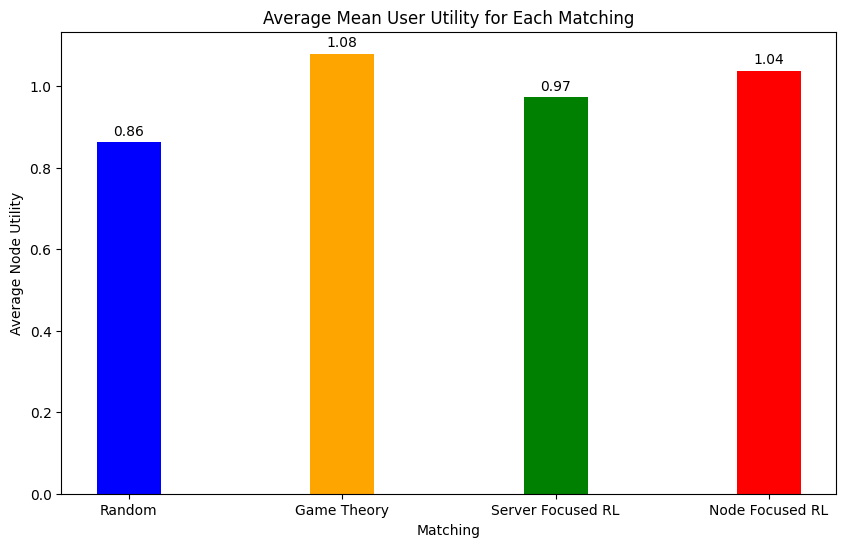
\includegraphics[width=0.9\textwidth]{figures/chapter3/Average_Mean_User_Utility.png}
    \caption{Μέση χρησιμότητα κόμβων ανά αλγόριθμο αντιστοίχισης}
    \label{fig14}
\end{figure}

\begin{figure}[H]
    \centering
    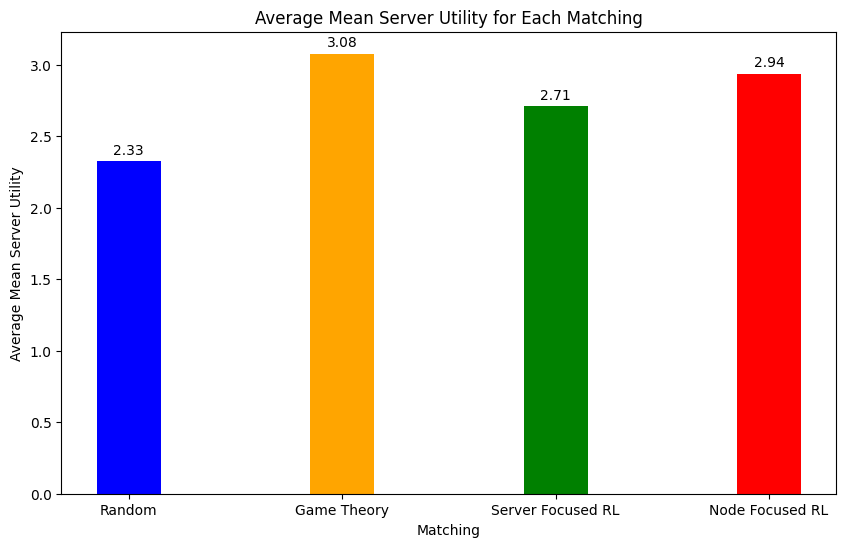
\includegraphics[width=0.9\textwidth]{figures/chapter3/Average_Mean_Server_Utility.png}
    \caption{Μέση χρησιμότητα εξυπηρετητών ανά αλγόριθμο αντιστοίχισης}
    \label{fig15}
\end{figure}

\newpage

Αντίστοιχα στα διαγράμματα \ref*{fig14} και \ref*{fig15}, μπορούμε να δούμε πώς ο αλγόριθμος Θεωρίας Παιγνίων έχει την καλύτερη επίδοση όσον αφορά τις χρησιμότητες κόμβων και εξυπηρετητών. Με σειρά ακολουθούν ο αλγόριθμος Ενισχυτικής Μάθησης ως προς χρησιμότητα κόμβων, ο αλγόριθμος Ενισχυτικής Μάθησης ως προς χρησιμότητα εξυπηρετητών και τέλος η Τυχαία Αντιστοίχιση. Η σύγκριση στα δύο αυτά διαγράμματα αποτελεί ίσως την πιο σημαντική σύγκριση, αφού όλες οι αποφάσεις για την αντιστοίχιση παίρνονται ώστε να μεγιστοποιηθούν οι χρησιμότητες. Έτσι εδώ φαίνεται ξεκάθαρα η υπεροχή του αλγορίθμου Θεωρίας Παιγνίων έναντι των υπολοίπων.

Όσον αφορά τον χρόνο εκτέλεσης της αντιστοίχισης για τους αλγορίθμους μας,στο διάγραμμα \ref{fig16} βλέπουμε πως η Τυχαία Αντιστοίχιση προφανώς διαθέτει τον πιο γρήγορο μηχανισμό, ακολουθούμενη από τον αλγόριθμο Ενισχυτικής Μάθησης ως προς χρησιμότητα κόμβων.

\begin{figure}[ht]
    \centering
    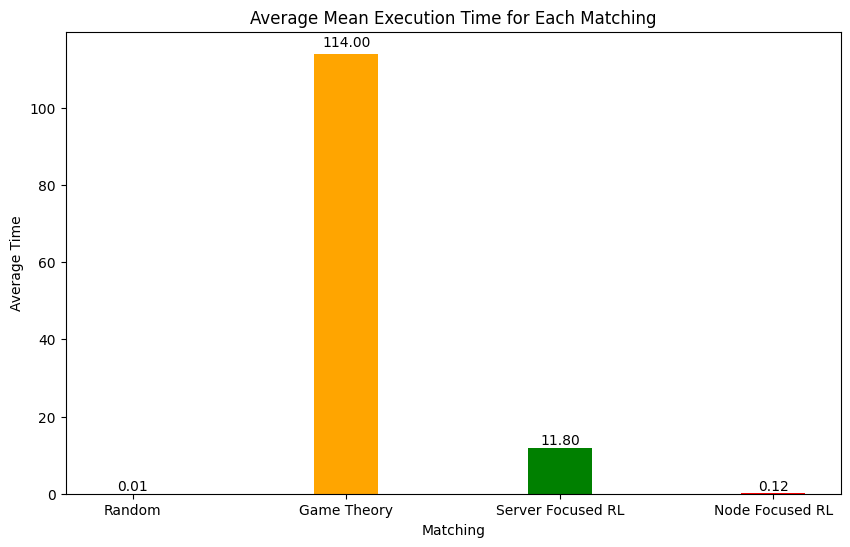
\includegraphics[width=\textwidth]{figures/chapter3/Average_Time.png}
    \caption{Μέσος χρόνος εκτέλεσης ανά αλγόριθμο αντιστοίχισης}
    \label{fig16}
\end{figure}

\newpage

\begin{figure}[H]
    \centering
    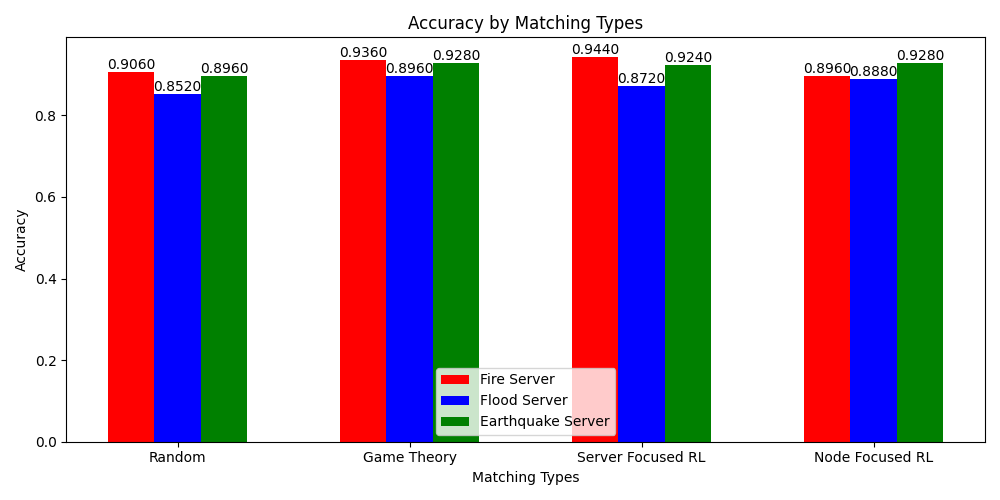
\includegraphics[width=\textwidth]{figures/chapter3/accuracy_plot.png}
    \caption{Μέση ακρίβεια εξυπηρετητών (ανά καταστροφή) για κάθε αλγόριθμο αντιστοίχισης}
    \label{fig50}
\end{figure}

\begin{figure}[H]
    \centering
    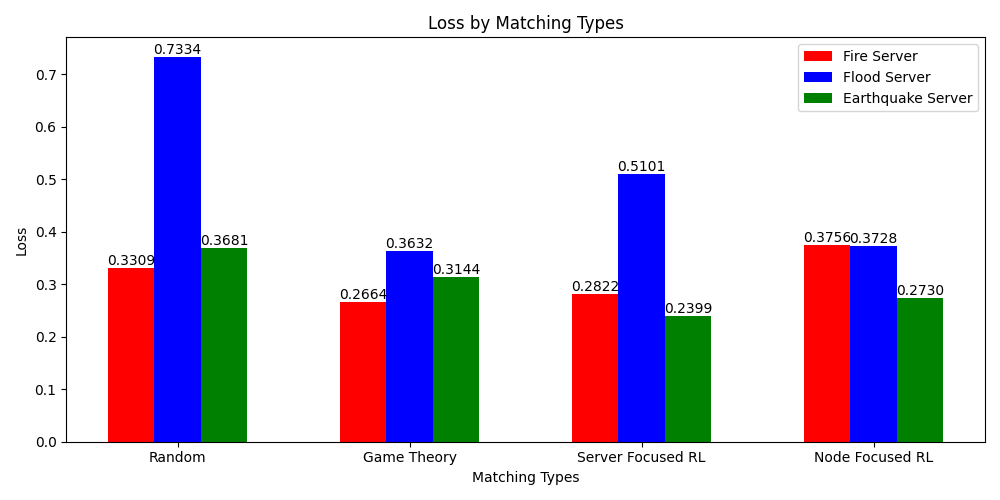
\includegraphics[width=\textwidth]{figures/chapter3/loss_plot.png}
    \caption{Μέση απώλεια εξυπηρετητών (ανά καταστροφή) για κάθε αλγόριθμο αντιστοίχισης}
    \label{fig51}
\end{figure}

\newpage

Για την επίδοση των αλγορίθμων αντιστοίχισης ως προς την Ομοσπονδιακή Μάθηση, θα πρέπει να εξετάσουμε την ακρίβεια και την απώλεια που πετυχαίνουν, όπως αυτές φαίνονται στα διαγράμματα \ref*{fig50} και \ref*{fig51}. Ο αλγόριθμος Θεωρίας Παιγνίων καταφέρνει κατά μέσο όρο να έχει την μικρότερη απώλεια στους τρεις εξυπηρετητές του, ακολουθούμενος από τους αλγορίθμους Ενισχυτικής Μάθησης. Είναι αξιοσημείωτο πως η Τυχαία Αντιστοίχιση παραμένει σχετικά κοντά στους αλγορίθμους μας, παρότι είναι το σημείο αναφοράς μας. Αυτό συμβαίνει επειδή στη διαδικασία της Ομοσπονδιακής Μάθησης συμπεριλαμβάνουμε έναν μηχανισμό ανάθεσης βαρών στους κόμβους μας, ανάλογα με την πληροφορία που διαθέτουν για τον εξυπηρετητή που έχουν συνδεθεί. Έτσι, κόμβοι με λίγη (ή και καθόλου χρήσιμη) πληροφορία θα επηρεάσουν πολύ λίγο την εκμάθηση του μοντέλου. Σε συνδυασμό με την πληροφορία που διαθέτει ο κάθε εξυπηρετητής, η Τυχαία Αντιστοίχιση επιτυγχάνει σεβαστές επιδόσεις παρά την απλότητα της. 
\chapter{Μετανοητική Μάθηση}

Σε αυτό το κεφάλαιο της διπλωματικής εργασίας θα μελετήσουμε έναν αλγόριθμο Μετανοητικής Μάθησης και θα τον συγκρίνουμε με τον αλγόριθμο Θεωρίας Παιγνίων που αναπτύξαμε στο κεφάλαιο 2. Η Μετανοητική Μάθηση (Regret Learning) είναι μια έννοια που ριζώνει στη θεωρία παιγνίων και τη μηχανική μάθηση, ιδιαίτερα σημαντική στο πλαίσιο επαναλαμβανόμενων παιγνίων και της ενεργής μάθησης. Εστιάζει στην ελαχιστοποίηση της ενοχής (μετάνοια), ορισμένης ως η διαφορά μεταξύ της απόδοσης μιας στρατηγικής λήψης αποφάσεων και της βέλτιστης στρατηγικής με βάση την αναδρομική θεώρηση, σε επαναλαμβανόμενες αλληλεπιδράσεις ή επαναλήψεις. 

Υπάρχουν δύο κύριοι τύποι ενοχής: η εξωτερική ενοχή, η οποία μετράει πόσο χειρότερα απέδωσε μια στρατηγική σε σύγκριση με την καλύτερη σταθερή δράση με βάση την αναδρομική θεώρηση, και η εσωτερική ενοχή, η οποία συγκρίνει την απόδοση με την καλύτερη προσαρμοστική πολιτική, όπου ο παίκτης θα μπορούσε να αλλάξει δράσεις με βάση τα προηγούμενα αποτελέσματα. Αλγόριθμοι ελαχιστοποίησης της ενοχής σχεδιάζονται για να ενημερώνουν τις πιθανότητες των δράσεων με βάση τις προηγούμενες αποδόσεις, ώστε να ελαχιστοποιήσουν την ενοχή. Αυτοί οι αλγόριθμοι έχουν εφαρμογές σε διάφορους τομείς, συμπεριλαμβανομένης της ενεργής μάθησης, όπου βοηθούν τους αλγορίθμους να μαθαίνουν από διαδοχικά δεδομένα σε αντίπαλα περιβάλλοντα, όπως η online διαφήμιση, στη θεωρία παιγνίων, ιδιαίτερα σε επαναλαμβανόμενα παίγνια όπου οι παίκτες προσαρμόζουν τις στρατηγικές τους με βάση τα προηγούμενα αποτελέσματα, και στη μάθηση με ενίσχυση, όπου οι πράκτορες μαθαίνουν πολιτικές για τη μεγιστοποίηση των ανταμοιβών με την πάροδο του χρόνου.

Τα οφέλη της Μετανοητικής Μάθησης περιλαμβάνουν την προσαρμοστικότητα, καθώς οι αλγόριθμοι μπορούν να προσαρμοστούν σε μεταβαλλόμενα περιβάλλοντα και να αποδώσουν καλά υπό διάφορες συνθήκες, και τη στιβαρότητα, που τους επιτρέπει να αντιμετωπίζουν αντιπαλικές καταστάσεις όπου οι αντίπαλοι μπορεί να προσπαθήσουν να εκμεταλλευτούν αδυναμίες. Τα θεωρητικά θεμέλια της ελαχιστοποίησης της ενοχής περιλαμβάνουν τη θεωρία πιθανοτήτων, την κυρτή ανάλυση και τη βελτιστοποίηση, με βασικά αποτελέσματα που συχνά παρέχουν όρια στην ενοχή που μπορεί να επιτευχθεί από συγκεκριμένους αλγόριθμους. Συνολικά, η μάθηση με βάση την ενοχή προσφέρει ένα στιβαρό πλαίσιο για τη λήψη αποφάσεων σε αβέβαια και αντιπαλικά περιβάλλοντα, διασφαλίζοντας ότι οι στρατηγικές αποδίδουν βέλτιστα με την πάροδο του χρόνου, ελαχιστοποιώντας το χάσμα μεταξύ της πραγματικής και της ιδανικής απόδοσης.

Μέχρι τώρα μελετούσαμε το πως θα πρέπει να κατανεμηθούν οι κόμβους στους εξυπηρετητές για να επιτύχουμε το καλύτερο δυνατό αποτέλεσμα στην Ομοσπονδιακή Μάθηση. Στο κομμάτι που ακολουθεί, αυξάνουμε το χώρο ενεργειών του κάθε κόμβου, δηλαδή του επιτρέπουμε να αλλάξει τιμές στα βασικά του μεγέθη επιλέγοντας πόσους πόρους θα θέλει ο ίδιος να διαθέσει για την Ομοσπονδιακή Μάθηση. Παρακάτω θα δούμε και πιο αναλυτικά τις παραμέτρους τις οποίες ο κάθε κόμβος μπορεί να μεταβάλλει για το συμφέρον του. Πολυδιάστατα, σαν αυτό, προβλήματα αυξάνουν πολύ σε πολυπλοκότητα όσο αυξάνεται και ο χώρος καταστάσεων που μπορούμε να έχουμε. Όμως, μπορούν να μας δώσουν και μεγάλα κέρδη σε χρησιμότητα, αφού εκ' φύσεως ο κάθε κόμβος έχει διαφορετικές βλέψεις και συμφέροντα σε ένα περιβάλλον Ομοσπονδιακής Μάθησης.

\section{Περιγραφή Αλγορίθμου Μετανοητικής Μάθησης}

Όπως αναφέραμε, πλέον κάθε κόμβος μπορεί να ελέγχει σε μεγαλύτερο βαθμό την συμπεριφορά του εντός του οικοσυστήματος. Συγκεκριμένα, μπορεί να προσαρμόζει τους διαθέσιμους πόρους του για να μεγιστοποιήσει την οφέλειά του, δηλαδή να αλλάξει την ισχύ μετάδοσης $P_{n,s}$, την συχνότητα του ρολογιού της ΚΜΕ του $f_n$ και το μέγεθος του συνόλου δεδομένων που θα διαθέσει στην μάθηση $D_n$.

Για να μοντελοποιήσουμε πιο ρεαλιστικά το οικοσύστημά μας, αλλάζουμε λίγο τα εμπλακώμενα μεγέθη που είδαμε στο κεφάλαιο 2. Έτσι, αντί για ποιότητα δεδομένων $d_n$, ενσωματώνουμε την παράμετρο $D_n$ στην πληρωμή που λαμβάνει ένας κόμβος από τον εξυπηρετητή. Δηλαδή όσο περισσότερα δεδομένα προσφέρει ένας κόμβος στον εξυπηρετητή του, τόσο καλύτερες απολαβές θα έχει. Αντίστοιχα, ενσωματώνουμε και την παράμετρο $f_n$ στην πληρωμή από τον εξυπηρετητή. Επιπλέον, κάθε κόμβος λαμβάνει απολαβές από τον εξυπηρετητή ανάλογα με τη σημασία του, αφού ένας εξυπηρετητής δεν θα ήθελε να πληρώνει το ίδιο έναν σημαντικό και έναν όχι τόσο σημαντικό κόμβου. Οπότε, με βάση τις παραπάνω παρατηρήσεις, διαμορφώνουμε την κανονικοποιημένη πληρωμή του κόμβου από τον εξυπηρετητή ως:

\vspace{-5pt}

\begin{equation}
\hat{Pnt}_{n,s}=\frac{c_{n,s}\times current\_fn*ud_n}{max\_f_n\times max\_d_n}
\label{eq20}
\end{equation}

\vspace{-3pt}

\noindent
όπου $c_{n,s}$ η σημασία δεδομένων του κόμβου, $current\_fn$ η τιμή της συχνότητας της ΚΜΕ που επιλέγει ο κόμβος να χρησιμοποιήσει, $ud_n$ το μέγεθος του συνόλου δεδομένου που επιλέγει ο κόμβος να διαθέσει, $max\_fn$ η μέγιστη συχνότητα της ΚΜΕ του κόμβου και $max\_dn$ το μέγιστο σύνολο δεδομένων που διαθέτει ο κόμβος.

Αντίστοιχα για τα υπόλοιπα μεγέθη που μελετήσαμε, τα κανονικοποιούμε με τον ίδιο τρόπο και έχουμε τις παρακάτω εξισώσεις:

\vspace{-5pt}

\begin{equation}
\hat{R}_{n,s} = \frac{R_{n,s}}{Rmax_{n,s}}
\label{eq21}
\end{equation}

\vspace{-3pt}

\[R_{n,s} = B \log_2(1 + \frac{g_{n,s}\times current\_P_{n,s}}{\sum \limits_{n'\in s, n'\neq n} g_{n',s}P_{n',s} + g_{n,s}\times current\_P_{n,s} + I_0}) \quad [bps]\]

\[Rmax_{n,s} = B \log_2(1 + \frac{g_{n,s}\times max\_P_{n,s}}{\sum \limits_{n'\in s, n'\neq n} g_{n',s}P_{n',s} + g_{n,s}\times max\_P_{n,s} + I_0}) \quad [bps]\]

\noindent
όπου $current\_P_{n,s}$ δηλώνει την ισχύ μετάδοσης που επιλέγει ο κόμβος, $max\_P_{n,s}$ είναι η μέγιστη ισχύ μετάδοσης που μπορεί να διαθέσει ο κόμβος και άρα $R_{n,s}$ είναι ο ρυθμός μετάδοσης που πετυχαίνει ο κόμβος και $Rmax_{n,s}$ είναι ο μέγιστος ρυθμός μετάδοσης που μπορεί να πετύχει ο κόμβος με βάση την τωρινή κατάσταση του συστήματος.

\vspace{-5pt}

\begin{equation}
\hat{E}_n=\frac{\frac{a_n}{2}q_n\times ud_n\times current\_f_n^2}{\frac{a_n}{2}q_n\times max\_d_n\times max\_f_n^2} = \frac{ud_n\times current\_f_n^2}{max\_d_n\times max\_f_n^2}
\label{eq22}
\end{equation}

\vspace{-3pt}

\noindent
όπου $current\_fn$ η τιμή της συχνότητας της ΚΜΕ που επιλέγει ο κόμβος να χρησιμοποιήσει, $ud_n$ το μέγεθος του συνόλου δεδομένου που επιλέγει ο κόμβος να διαθέσει, $max\_fn$ η μέγιστη συχνότητα της ΚΜΕ του κόμβου και $max\_dn$ το μέγιστο σύνολο δεδομένων που διαθέτει ο κόμβος.

\vspace{-5pt}

\begin{equation}
\hat{E}_{n,s}=\frac{\frac{Z(\mathbf{w}n)\times current\_P{n,s}}{R_{n,s}}}{\frac{Z(\mathbf{w}n)\times max\_P{n,s}}{Rmax_{n,s}}} = \frac{current\_P{n,s}\times Rmax_{n,s}}{max\_P{n,s}\times R_{n,s}}
\label{eq23}
\end{equation}

\vspace{-3pt}

\noindent
όπου $current\_P_{n,s}$ δηλώνει την ισχύ μετάδοσης που επιλέγει ο κόμβος, $max\_P_{n,s}$ είναι η μέγιστη ισχύ μετάδοσης που μπορεί να διαθέσει ο κόμβος και άρα $R_{n,s}$ είναι ο ρυθμός μετάδοσης που πετυχαίνει ο κόμβος και $Rmax_{n,s}$ είναι ο μέγιστος ρυθμός μετάδοσης που μπορεί να πετύχει ο κόμβος με βάση την τωρινή κατάσταση του συστήματος.

Όπως γίνεται εμφανές από τις παραπάνω εξισώσεις, κάθε μία από τις παραμέτρους $P_{n,s}$, $f_n$, $ud_n$, όσο αυξάνονται, αυξάνουν με τη σειρά τους δύο μεγέθη, ένα θετικό και ένα αρνητικό. Επιπλέον, για την παράμετρο $P_{n,s}$ βλέπουμε πως η ισχύς της επηρεάζεται και από εξωτερικές παραμέτρους, δηλαδή από τις επιλογές των υπολοίπων κόμβων.

Συνεπώς θα πρέπει να οργανώσουμε μία νέα συνάρτηση χρησιμότητας η οποία θα αντικατοπτρίζει την συμπεριφορά αυτή τον μεγεθών, αλλά θα μας επιτρέπει και να μοντελοποιήσουμε την συμπεριφορά των κόμβων μας. Δηλαδή για παράδειγμα, κάποιος κόμβος, γνωρίζοντας την χρησιμότητά του, αν αυτή είναι χαμηλή, μπορεί να τον συμφέρει να αφιερώσει λιγότερους πόρους στην Ομοσπονδιακή Μάθηση, απ' ότι κάποιος κόμβος ο οποίος γνωρίζει πως μπορεί να επωφεληθεί από την διαδικασία. Έτσι ορίζουμε ως νέα συνάρτηση χρησιμότητας για μια παράμετρο την:

\vspace{-5pt}

\begin{equation}
Uparameter_{n,s}(pos, neg) = positive(pos, c_{n,s}, a) - negative(neg, a) 
\label{eq24}
\end{equation}

\vspace{-3pt}

\[positive(pos, c_{n,s}, a) = 2c_{n,s} + 1 - e^{(\frac{-pos}{a})}\]

\[negative(neg, a) = \frac{1}{1 + e^{(\frac{-neg}{a} + 3)}}\]

\noindent
όπου $pos$ είναι το κανονικοποιημένο θετικό μέγεθος της παραμέτρου και $neg$ το κανονικοποιημένο αρνητικό μέγεθος της παραμέτρου. Επιπλέον θέτοντας ως άνω όριο το $2c_{n,s} + 1$, εξασφαλίζουμε καλύτερες τιμές χρησιμότητας για τους πιο σημαντικούς κόμβους, δίνοντας έτσι προτεραιότητα σε αυτούς. Η παράμετρος $a$, όπως θα εξηγήσουμε και παρακάτω, μας επιτρέπει να ορίσουμε συγκεκριμένες συμπεριφορές για τους κόμβους μας, προσομοιώνοντας έτσι τις διαφορετικές επιθυμίες και συμφέροντα τους.

Συνεπώς η συνολική συνάρτηση χρησιμότητας είναι:

\vspace{-0.6cm}

\begin{equation}
U_{n,s} =  U\{P_{n,s}\}_{n,s}(\hat{R_{n,s}}, \hat{E_{n,s}}) + U\{f_n\}_{n,s}(\hat{Pnt}_{n,s}, \hat{E}_n) + U\{ud_n\}_{n,s}(\hat{Pnt}_{n,s}, \hat{E}_n)
\label{eq25}
\end{equation}

\vspace{-3pt}

\noindent
Όπως βλέπουμε τα μεγέθη $\hat{Pnt}_{n,s}$ και$\hat{E}_n$ συμμετέχουν και στην χρησιμότητα της παραμέτρου $f_n$ και στην χρησιμότητα της παραμέτρου $ud_n$. Για να λύσουμε το πρόβλημα αυτό θα πρέπει να δημιουργήσουμε τέσσερα νέα μεγέθη από τα δύο υπάρχοντα, όπου τα δύο θα αφορούν την παράμετρο $f_n$ και τα άλλα δύο την παράμετρο $ud_n$. Έτσι έχουμε:

\[\hat{Pnt}\{f_n\}_{n,s}=\frac{c_{n,s}\times current\_fn}{max\_f_n}\]

\[\hat{Pnt}\{ud_n\}_{n,s}=\frac{c_{n,s}\times ud_n}{max\_d_n}\]

\[\hat{E}\{f_n\}_n = \frac{current\_f_n^2}{max\_f_n^2}\]

\[\hat{E}\{ud_n\}_n = \frac{ud_n}{max\_d_n}\]

\noindent Και άρα πλέον η εξίσωση \ref{eq25} μπορεί να γραφεί ως:

\vspace{-0.6cm}

\begin{equation}
\begin{split}
    U_{n,s} =& U\{P_{n,s}\}_{n,s}(\hat{R_{n,s}}, \hat{E_{n,s}}) + U\{f_n\}_{n,s}(\hat{Pnt}\{f_n\}_{n,s}, \hat{E}\{f_n\}_n) +\\
    & U\{ud_n\}_{n,s}(\hat{Pnt}\{ud_n\}_{n,s}, \hat{E}\{ud_n\}_n)
\end{split}
\label{eq26}
\end{equation}

\vspace{-3pt}

Επιπροσθέτως, θα πρέπει να αναλύσουμε την λογική της παραμέτρου συμπεριφοράς $a$ για τις συναρτήσεις χρησιμότητας των κόμβων. Κάθε συνάρτηση της μορφής \ref{eq24} αποτελεί μία συνάρτηση με μορφή καμπάνας, δηλαδή εμφανίζει ένα ολικό μέγιστο (όχι στο άπειρο). Συγκεκριμένα αν το $a < 0.57$, το μέγιστο αυτό βρίσκεται εντός του $[0,1]$ που είναι και το διάστημα που μας ενδιαφέρει, αφού οι τιμές των μεγεθών μας είναι κανονικοποιημένες. Όσο μεγαλύτερη είναι η τιμή του $a$, τόσο πιο δεξιά θα βρίσκεται το μέγιστο και άρα θα ενθαρρύνεται ο κόμβος να αφιερώσει περισσότερους πόρους στην Ομοσπονδιακή Μάθηση για την συγκεκριμένη παράμετρο. Συνεπώς, θα πρέπει για κάθε κόμβου $n$ να δώσουμε για κάθε μία από τις παραμέτρους του μία κατάλληλη παράμετρο συμπεριφοράς $a$ με βάση την νοοτροπία του κόμβου, δηλαδή αν πιστεύει πως μπορεί να επωφεληθεί πολύ ή λίγο από την Ομοσπονδιακή Μάθηση και τον κάθε εξυπηρετητή. Άρα αναθέτουμε τις παραμέτρους συμπεριφοράς με τον εξής τρόπο:

\[a\{P_{n,s}\} = \text{random.uniform}\left(\max\left(a_1 \times c_{n,s} - a_3, a_3\right), a_1 \times c_{n,s}\right)\]

\[a\{f_n\} = \text{random.uniform}\left(\max\left(a_2 \times \sqrt{c_{n,s}} - a_3, a_3\right), a_2 \times \sqrt{c_{n,s}}\right)\]

\[a\{ud_n\} = \text{random.uniform}\left(\max\left(a_2 \times \sqrt{c_{n,s}} - a_3, a_3\right), a_2 \times \sqrt{c_{n,s}}\right)\]

\noindent
Με την κατανομή αυτή εξασφαλίζουμε πως οι κόμβους που έχουν να κερδίζουν περισσότερα από τους εξυπηρετητές (μεγαλύτερη σημασία δεδομένων) θα προτιμούν να αφιερώσουν μεγαλύτερο μέρος των διαθέσιμων πόρων τους, σε αντίθεση με τους λιγότερο σημαντικούς κόμβους, οι οποίοι γνωρίζουν πως δεν μπορούν να επωφεληθούν πολύ από την όλη διαδικασία και άρα είναι πιο διστακτικοί.

Αφού, λοιπόν, ορίσαμε την νέα συνάρτηση χρησιμότητας και τις παραμέτρους της μπορούμε να προχωρήσουμε στην ανάλυση και περιγραφή των αλγορίθμων που θα χρησιμοποιήσουμε. Θα μελετήσουμε τους εξής δύο αλγορίθμους: i) Μετανοητική Μάθηση Πλήρους Πληροφορίας ii) Μετανοητική Μάθηση Ελλιπούς Πληροφορίας. Ο πρώτος αλγόριθμος, έχοντας πλήρη γνώση των ενεργειών των υπολοίπων κόμβων εκμεταλλεύται την γνώση αυτή για να εντοπίσει τις βέλτιστες σε κάθε περίπτωση ενέργειες. Ο δεύτερος αλγόριθμος αντιπροσωπεύει ένα πιο ρεαλιστικό σενάριο, όπου ο κάθε κόμβος λαμβάνει την δική του ανατροφοδότηση, αλλά δεν γνωρίζει για τις ενέργειες των υπολοίπων κόμβων.

\textbf{Πλήρους Πληροφορίας:} Αρχικά, κατασκευάζουμε όλες τις πιθανές καταστάσεις που μπορεί να βρίσκεται ένας κόμβος, δηλαδή για κάθε εξυπηρετητή, για κάθε τιμή κάθε παραμέτρου. Αυτός είναι ο χώρος ενεργειών μας. Στην συνέχεια, αρχικοποιούμε το διάνυσμα πιθανοτήτων έχοντας όλες τις ενέργειες ισοπίθανες και το διάνυσμα μετάνοιας σε μηδενικές τιμές. Έτσι ξεκινάμε επαναληπτικά να ακολουθούμε την εξής διαδικασία: Σε κάθε επανάληψη, οι $N$ κόμβους μας διαλέγουν ο καθένας, με βάση το διάνυσμα πιθανοτήτων τους, μια ενέργεια. Εκτελούν τη συγκεκριμένη ενέργεια και έπειτα ενημερώνουν το διάνυσμα μετάνοιας τους για κάθε πιθανή ενέργεια με τον παρακάτω τρόπο:

\vspace{-5pt}

\begin{equation}
\begin{split}
    \text{regret\_vector}(user, action) =& \left(1 - l(t)\right) \text{regret\_vector}(user, action)\\
    &+ \text{utility\_difference}(action, taken\_action)
\end{split}
\label{eq27}
\end{equation}

\vspace{-3pt}

\[l(t) = \frac{1}{t}\]

\noindent
όπου $l(t)$ είναι ο ρυθμός εκμάθησης, δηλαδή δηλώνει πόσο σημαντική είναι η πληροφορία που έχουμε μέχρι τώρα και πόσο οι νέες πληροφορίες που μαθαίνουμε. Επίσης η $\text{utility\_difference}(action, taken\_action)$ μας δίνει την διαφορά σε χρησιμότητα του κόμβου μεταξύ της ενέργειας που μελετάμε και της ενέργειας που εκτελέσαμε στην τελευταία επανάληψη. 

Αφού ενημερώσουμε έτσι το διάνυσμα μετάνοιας του κάθε κόμβου, ενημερώνουμε και το διάνυσμα πιθανοτήτων ως εξής:

\vspace{-5pt}

\begin{equation}
P(u,action) =
\begin{cases}
    0 & \text{if } S_u = 0 \\
    \frac{\max(0, regret\_vector(user, action))}{S_u} & \text{if } S_u > 0
\end{cases}
\label{eq28}
\end{equation}

\vspace{-3pt}

\[S_u = \sum_{action \in actions} \max(0, regret\_vector(user, action))\]

Η διαδικασία επαναλαμβάνεται μέχρι να πετύχουμε σύγκλιση, η οποία εξασφαλίζεται εφ' όσον για κάθε κόμβου υπάρχει μία ενέργεια η οποία επιλέγεται με πιθανότητα άνω του 50\%. Σε τέτοια περίπτωση σταματάμε την διαδικασία και επιλέγουμε για κάθε κόμβου την πιθανότερη ενέργειά του καταλήγοντας στο τελικό μας αποτέλεσμα.

\newpage

\begin{algorithm}[h]
\caption{Αλγόριθμος Μετανοητική Μάθησης Πλήρους Πληροφορίας} \label{algorithm 5}
\begin{algorithmic}[1]
\STATE \textbf{\underline{Είσοδος:}} ${L_n, a_n, q_n, D_n, f_n, \mathbf{w}n}{\forall n\in \mathcal{N}}, {L_k}_{\forall k \in \mathcal{K}}$, παράμετροι συμπεριφοράς
\STATE \textbf{\underline{Έξοδος:}} \text{Αποτελέσματα Αντιστοίχισης και Ενεργειών} $M$
\STATE \textbf{\underline{Αρχικοποίηση:}} $\forall n$ δημιουργούμε όλες τις πιθανές ενέργειες του, $\forall n, \forall actions$ αρχικοποιούμε τα διανύσματα μετάνοιας σε μηδενικές τιμές και τα διανύσματα πιθανότητας σε ίσες τιμές
\WHILE{no convergence}
\FOR{$n \in \mathcal{N}$}
\STATE Ο κόμβος $n$ επιλέγει με βαρύτητα το διάνυσμα πιθανοτήτων του μια ενέργεια και την εκτελεί.
\ENDFOR
\FOR{$n \in \mathcal{N}$}
\STATE Ο κόμβος $n$ ανανεώνει με βάση την Εξίσωση \ref{eq27} το διάνυσμα μετανοιών του.
\STATE Ο κόμβος $n$ ανανεώνει με βάση την Εξίσωση \ref{eq28} το διάνυσμα πιθανοτήτων του.
\ENDFOR
\ENDWHILE
\FOR{$n \in \mathcal{N}$}
\STATE Ο κόμβος $n$ επιλέγει και εκτελεί την πιο πιθανή ενέργειά του.
\ENDFOR
\end{algorithmic}
\end{algorithm}

\textbf{Ελλιπούς Πληροφορίας:} Αρχικά κατασκευάζουμε και πάλι τον χώρο ενεργειών. Στην συνέχεια, αρχικοποιούμε το διάνυσμα πιθανοτήτων έχοντας όλες τις ενέργειες ισοπίθανες, το διάνυσμα μετάνοιας σε μηδενικές τιμές και το διάνυσμα χρησιμότητας στις αντίστοιχες τιμές χρησιμότητας χωρίς εξωτερικότητα. Έτσι ξεκινάμε επαναληπτικά να ακολουθούμε την εξής διαδικασία: Σε κάθε επανάληψη, οι $N$ κόμβους μας διαλέγουν ο καθένας, με βάση το διάνυσμα πιθανοτήτων τους, μια ενέργεια. Εκτελούν τη συγκεκριμένη ενέργεια και έπειτα ενημερώνουν το διάνυσμα χρησιμότητάς τους για τη συγκεκριμένη ενέργεια με τον παρακάτω τρόπο:

\vspace{-5pt}

\begin{equation}
    \text{utilities\_vector}(u,action\_taken) = 0.5 \times \left(\text{current\_utility} + \text{utilities\_vector}(u,action\_taken)\right)
\label{eq29}
\end{equation}

\vspace{-3pt}

\noindent
όπου το current\_utility αναφέρεται στην χρησιμότητα που έλαβε ο κόμβος $n$ εκτελώντας την τελευταία ενέργεια που επέλεξε. Στη συνέχεια ενημερώνουμε το διάνυσμα μετάνοιας του κόμβου για κάθε πιθανή ενέργεια ως:

\vspace{-5pt}

\begin{equation}
\begin{split}
    \text{regret\_vector}(user, action) =& \left(1 - l(t)\right) \text{regret\_vector}(user, action)\\
    &+ \text{current\_utility} - \text{utilities\_vector}(u,action)
\end{split}
\label{eq30}
\end{equation}

\vspace{-3pt}

\[l(t) = \frac{1}{t}\]

όπου το current\_utility αναφέρεται στην χρησιμότητα που έλαβε ο κόμβος $n$ εκτελώντας την τελευταία ενέργεια που επέλεξε. Τέλος ενημερώνουμε το διάνυσμα πιθανοτήτων ως:

\vspace{-5pt}

\begin{equation}
    \text{probabilities}(u,action) = \text{boltzmann\_gibbs\_vector}_u(action)
\label{eq31}
\end{equation}

\vspace{-3pt}

\[
\text{boltzmann\_gibbs\_vector}_u(action) = \frac{e^{\max(0, regret\_vector(user, action))/k_m}}{S_u}
\]

\[S_u = \sum_{action \in actions} \max(0, e^{\max(0, regret\_vector(user, action))/k_m})\]

Όπως και προηγουμένως, διαδικασία επαναλαμβάνεται μέχρι να πετύχουμε σύγκλιση, η οποία εξασφαλίζεται εφ' όσον για κάθε κόμβου υπάρχει μία ενέργεια η οποία επιλέγεται με πιθανότητα άνω του 50\%. Σε τέτοια περίπτωση σταματάμε την διαδικασία και επιλέγουμε για κάθε κόμβου την πιθανότερη ενέργειά του καταλήγοντας στο τελικό μας αποτέλεσμα.

\begin{algorithm}[h]
\caption{Αλγόριθμος Μετανοητική Μάθησης Ελλιπούς Πληροφορίας} \label{algorithm 6}
\begin{algorithmic}[1]
\STATE \textbf{\underline{Είσοδος:}} ${L_n, a_n, q_n, D_n, f_n, \mathbf{w}n}{\forall n\in \mathcal{N}}, {L_k}_{\forall k \in \mathcal{K}}$, παράμετροι συμπεριφοράς
\STATE \textbf{\underline{Έξοδος:}} \text{Αποτελέσματα Αντιστοίχισης και Ενεργειών} $M$
\STATE \textbf{\underline{Αρχικοποίηση:}} $\forall n$ δημιουργούμε όλες τις πιθανές ενέργειες του, $\forall n, \forall actions$ αρχικοποιούμε τα διανύσματα χρησιμότητας σε αντίστοιχες τιμές χρησιμότητας χωρίς εξωτερικότητα, τα διανύσματα μετάνοιας σε μηδενικές τιμές και τα διανύσματα πιθανότητας σε ίσες τιμές
\WHILE{no convergence}
\FOR{$n \in \mathcal{N}$}
\STATE Ο κόμβος $n$ επιλέγει με βαρύτητα το διάνυσμα πιθανοτήτων του μια ενέργεια και την εκτελεί.
\ENDFOR
\FOR{$n \in \mathcal{N}$}
\STATE Ο κόμβος $n$ ανανεώνει με βάση την Εξίσωση \ref{eq29} την τιμή τους δινύσματος χρησιμότητας για την συγκεκριμένη ενέργεια.
\STATE Ο κόμβος $n$ ανανεώνει με βάση την Εξίσωση \ref{eq30} το διάνυσμα μετανοιών του.
\STATE Ο κόμβος $n$ ανανεώνει με βάση την Εξίσωση \ref{eq31} το διάνυσμα πιθανοτήτων του.
\ENDFOR
\ENDWHILE
\FOR{$n \in \mathcal{N}$}
\STATE Ο κόμβος $n$ επιλέγει και εκτελεί την πιο πιθανή ενέργειά του.
\ENDFOR
\end{algorithmic}
\end{algorithm}
\vspace{-7pt}

\textbf{Σύγκλιση:} Οι συγγραφείς του [enter reference here] δηλώνουν πως για τον αλγόριθμο Πλήρους Πληροφορίας, θα επιτευχθεί η σύγκλιση εφόσον ακολουθηθεί η διαδικασία της Μετανοητικής Μάθησης. Για τον αλγόριθμο Ελλιπούς Πληροφορίας, αναφέρουν πως για να επιτευχθεί η σύγκλιση όπως στον αλγόριθμο Πλήρους Πληροφορίας, θα πρέπει η συνάρτηση χρησιμότητας $U$ να αποτελεί συνάρτηση Lipschitz. Συγκεκριμένα, στην περίπτωσή μας, μας αφορούν οι συναρτήσεις:

\[f(x) = 2 \cdot c_{n,s} + 1 - e^{-\frac{x}{a}}, g(x) = \frac{1}{1 + e^{-\frac{x}{a} + 3}}\]

Μια συνάρτηση είναι Lipschitz, αν και μόνο εάν αυτή έχει φραγμένη παράγωγο. Και οι δύο αυτές συναρτήσεις (και συγκεκριμένα στο $[0,\inf)$) έχουν φραγμένη παράγωγο και άρα είναι συναρτήσεις Lipschitz. Επιπλέον, αν έχουμε δύο συναρτήσεις Lipschitz και τις προσθέσουμε (ή αφαιρέσουμε) η νέα συνάρτηση προφανώς θα είναι και αυτή Lipschitz. Συνεπώς, οι συναρτήσεις μας της μορφής \ref{eq24} είναι Lipschitz. Αντίστοιχα, εφαρμόζοντας τον ίδιο κανόνα προκύπτει ότι και η \ref{eq26} θα είναι Lipschitz, εξασφαλίζοντας την ορθή λειτουργεία του αλγορίθμου Ελλιπούς Πληροφορίας και την σύγκλισή του.

\section{Υλοποίηση}

Τόσο για τον αλγόριθμο Πλήρους Πληροφορίας όσο και για τον αλγόριθμο Ελειπούς Πληροφορίας, θα πρέπει όπως και πριν να εξασφαλίσουμε τον ορθό διαμοιρασμό των δεδομένων, με συνεπή τρόπο για να μπορούμε να πάρουμε συγκρίσιμα αποτελέσματα. Αντίστοιχα, και πάλι θα πρέπει να φροντίσουμε οι κόμβους μας να αποτελούν όμοια αντικείμενα σε κάθε περίπτωση ώστε οι αλγόριθμοι να συγκρίνονται πάνω στο ίδιο περιβάλλον.

Κάθε αντικείμενο κόμβου, θα έχει τρία βασικά χαρακτηριστικά:
\begin{itemize}
    \item $Ptransmit$: Η ισχύς μετάδοσης που χρησιμοποιείται (W)
    \item $fn$: Οι κύκλοι/δευτερόλεπτο που διαθέτει ο επεξεργαστής
    \item $used\_datasize$: Το ποσοστό του συνολικού συνόλου δεδομένων που χρησιμοποιεί ο κόμβος για την εκπαίδευση του μοντέλου του   
\end{itemize}

Αυτά προφανώς μεταβάλλονται στους αλγορίθμους Μετανοητικής Μάθησης. Αντίθετα, στον αλγόριθμο Θεωρίας Παιγνίων θέτουμε τις τιμές:
\begin{itemize}
    \item $Ptransmit = P_{max} = 2 Watt$
    \item $fn = fn_{max} = 2 GHz$
    \item $used\_datasize = 1$   
\end{itemize}
οι οποίες μένουν οριστικά και δεν αλλάζουν στον συγκεκριμένο αλγόριθμο.

Τέλος, όπως είδαμε παραπάνω (Εξίσωση \ref{eq24}), κάθε ένα ζευγάρι κόμβου-εξυπηρετητή, δημιουργεί τρεις συναρτήσεις χρησιμότητας με βάση την χρησιμότητά του και μια παράμετρο α, η οποία επίσης εξαρτάται επίσης από τη χρησιμότητά του. Όπως είδαμε, για την παραγωγή των παραμέτρων $a$ σε κάθε περίπτωση χρειαζόμαστε τις σταθερές $a_1$, $a_2$ και $a_3$. Στην περίπτωσή μας, για να έχουμε την επιθυμητή συμπεριφορά των συναρτήσεων χρησιμότητας στο διάστημα [0,1] θέτουμε:

\begin{itemize}
    \item $a_1 = 0.4$
    \item $a_2 = 0.57$
    \item $a_3 = 0.05$
\end{itemize}

\section{Αποτελέσματα}

Για να μελετήσουμε την συμπεριφορά του συστήματός μας σε διάφορες καταστάσεις, εκτελούμε την διαδικασία της αντιστοίχισης και της Ομοσπονδιακής Μάθησης πολλαπλές φορές για διαφορετικό πλήθος κόμβων. Κατά την διάρκεια της εκτέλεσης, κρατάμε πληροφορία για την ποιότητα της αντιστοίχισης αλλά και την εξέλιξη της Ομοσπονδιακής Μάθησης, ώστε έπειτα από τα αρχεία αυτά να μπορούμε να κατασκευάσουμε τα απαραίτητα διαγράμματα για να κάνουμε πιο κατανοητή την συμπεριφορά του οικοσυστήματος μας.

Συνεπώς, όσον αφορά την επίδοση της Ομοσπονδιακής Μάθησης για τον κάθε εξυπηρετητή βλέπουμε το εξής:

\begin{figure}[ht]
    \centering
    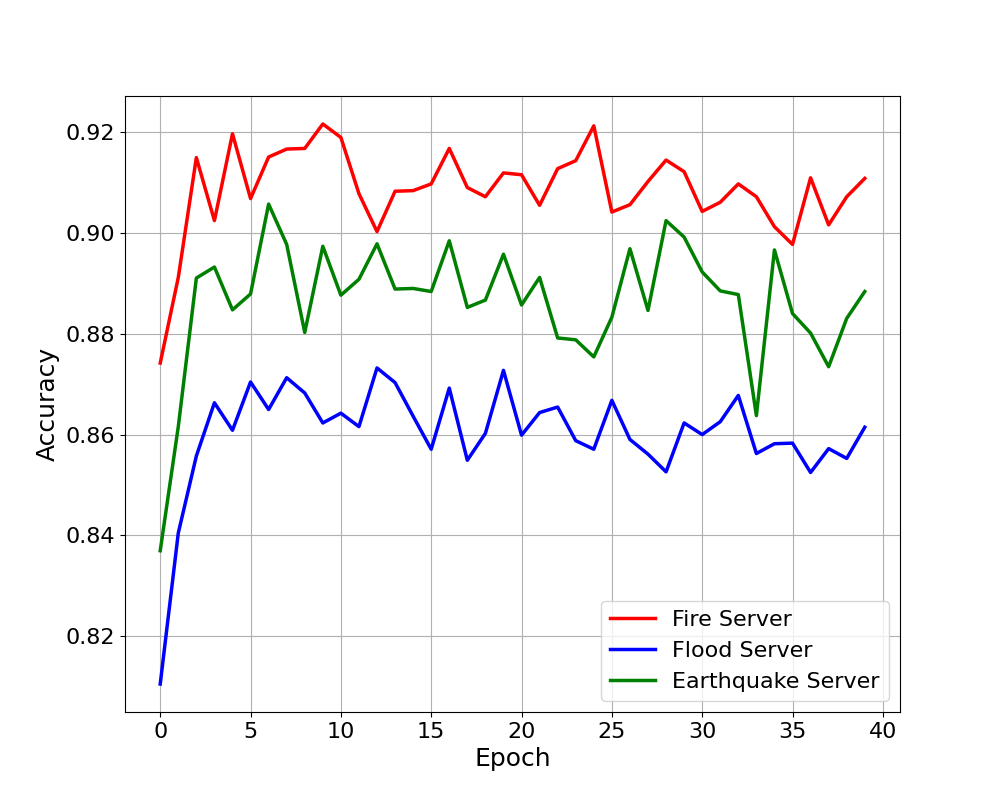
\includegraphics[width=\textwidth]{figures/chapter4/Server_Accuracies.png}
    \caption{Ακρίβεια Εξυπηρετητών στην Μετανοητική Μάθηση}
    \label{fig17}
\end{figure}

\begin{figure}[ht]
    \centering
    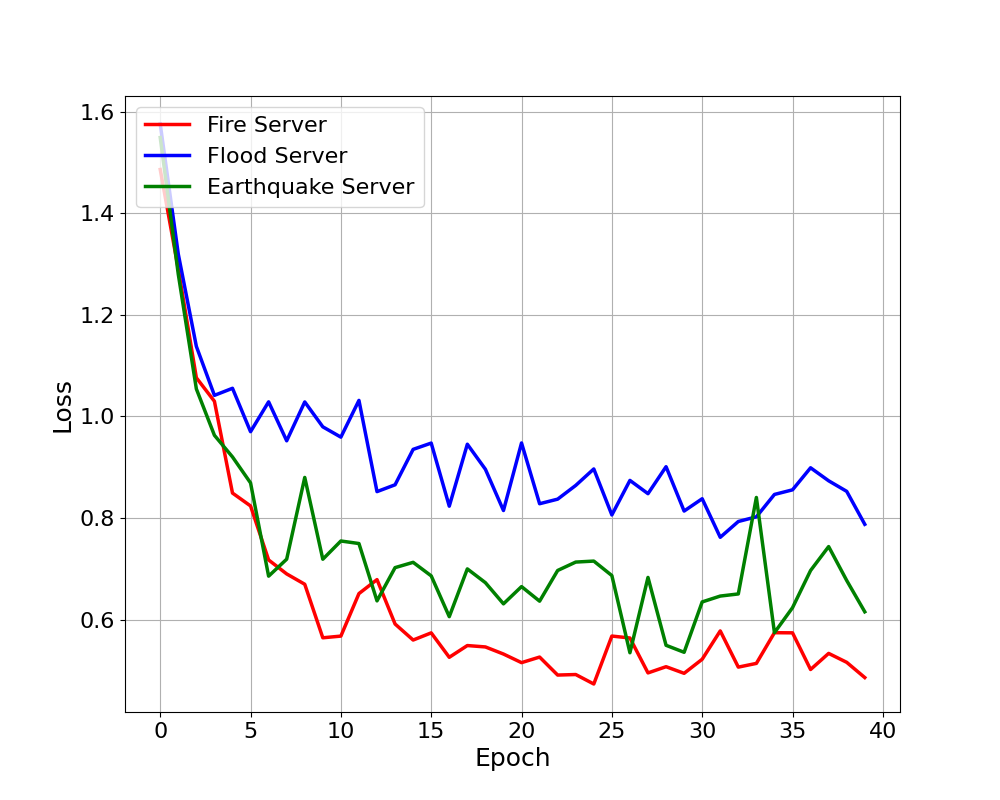
\includegraphics[width=\textwidth]{figures/chapter4/Server_Losses.png}
    \caption{Απώλεια Εξυπηρετητών στην Μετανοητική Μάθηση}
    \label{fig18}
\end{figure}

Όπως βλέπουμε στα σχήματα \ref{fig17}, \ref{fig18}, παρατηρούμε παρόμοια συμπεριφορά με τις προηγούμενες τεχνικές αντιστοίχισης. Όπως και σε προηγούμενες περιπτώσεις, έχουμε $Datasize_{fire} > Datasize_{flood} >Datasize_{earthquake}$, και επιπλέον ο εντοπισμός της φωτιάς είναι ένα πιο εύκολο πρόβλημα από ότι μιας πλημμύρας, αφού σε πλημμύρες έχουμε πιο ουδέτερα χρώματα, ενώ σε φωτιές πιο έντονα χρώματα και μεγάλες αλλαγές φωτεινότητας και σε σεισμούς πιο γήινα και ξηρά χρώματα. Επιπλέον, πολλές από τις ουδέτερες φωτογραφίες είναι πιο κοντά σε φωτογραφίες από πλημμύρες από ότι σε σεισμούς ή φωτιές, με αποτέλεσμα η διάκριση των δύο άλλων καταστροφών να είναι πιο απλή. Συνεπώς, για αυτούς τους λόγους, όπως και σε προηγούμενες περιπτώσεις έχουμε την καλύτερη απόδοση στον εξυπηρετητή που ανιχνεύει φωτιές, έπειτα στον εξυπηρετητή που ανιχνεύει σεισμούς και τέλος στον εξυπηρετητή που ανιχνεύει πλημμύρες παρότι $Datasize_{flood} >Datasize_{earthquake}$. 

Αντίστοιχα, γιατ τις επιδόσεις των κόμβων, είναι εμφανές στα διαγράμματα \ref*{fig19} και \ref*{fig20}, πως έχουμε παρόμοια συμπεριφορά, μόνο που η ακρίβεια των κόμβων του εξυπηρετητή που ανιχνεύει για σεισμούς είναι μεγαλύτερη. Αυτό μας δείχνει πως παρότι οι κόμβους τοπικά πετυχαίνουν καλύτερα αποτελέσματα, ο εξυπηρετητής δυσκολεύεται να γενικεύσει από τα βάρη που λαμβάνει από τους κόμβους του. Παρολαυτά, είναι σημαντικό όμως να αναφέρουμε πως οι κόμβους και οι εξυπηρετητές φαίνεται να μαθαίνουν αποτελεσματικά τις ιδιότητες των εικόνων, με αποτέλεσμα να πετυχαίνουν αρκετά υψηλές τελικές ακρίβειες. 

\newpage

\begin{figure}[H]
    \centering
    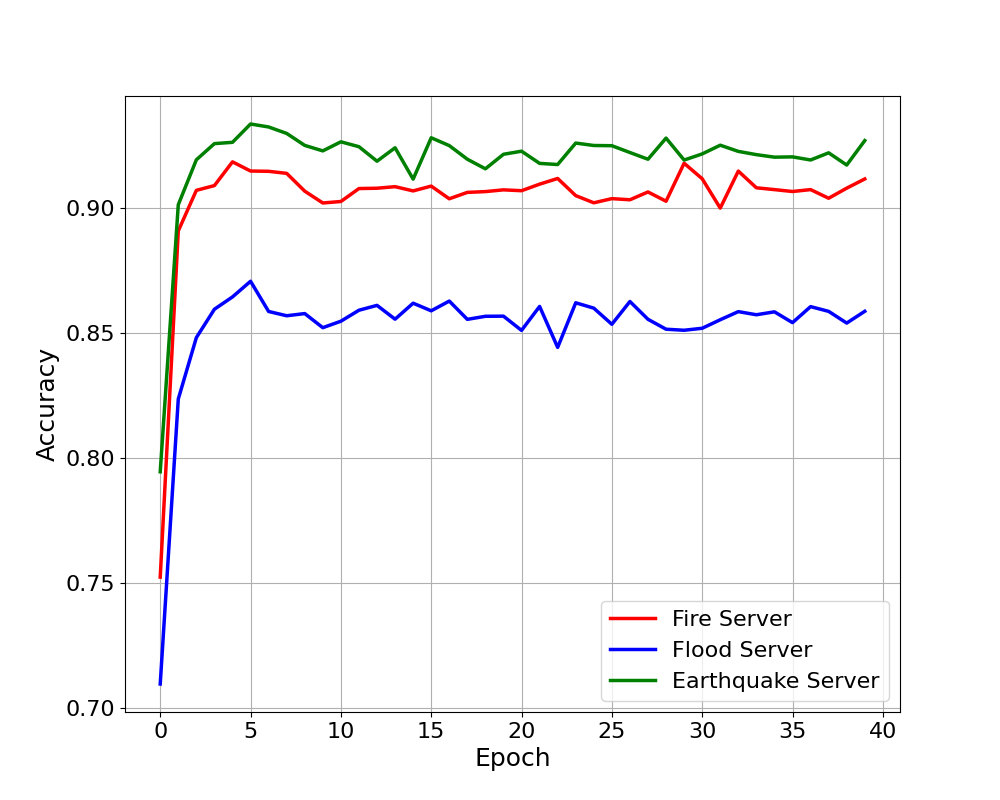
\includegraphics[width=0.85\textwidth]{figures/chapter4/User_Accuracies.png}
    \caption{Ακρίβεια κόμβων στην Μετανοητική Μάθηση}
    \label{fig19}
\end{figure}

\begin{figure}[H]
    \centering
    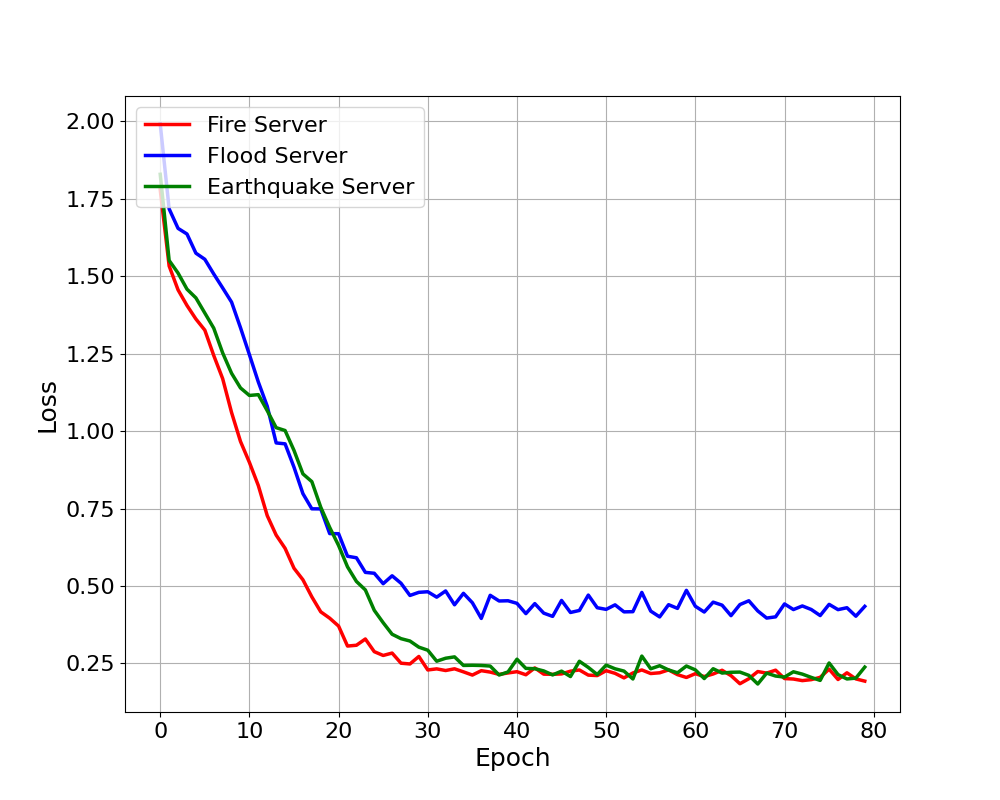
\includegraphics[width=0.85\textwidth]{figures/chapter4/User_Losses.png}
    \caption{Απώλεια κόμβων στην Μετανοητική Μάθηση}
    \label{fig20}
\end{figure}

\newpage

Όσον αφορά τις διαφορές μεταξύ των δύο αλγορίθμων Μετανοητικής Μάθησης, αλλά και όσον αφορά τις διαφορετικές περιοχές (Αστική Περιοχή, Προάστια, Αγοριτκή Περιοχή) παρατηρούμε τις εξής διαφορές:

\begin{figure}[H]
    \centering
    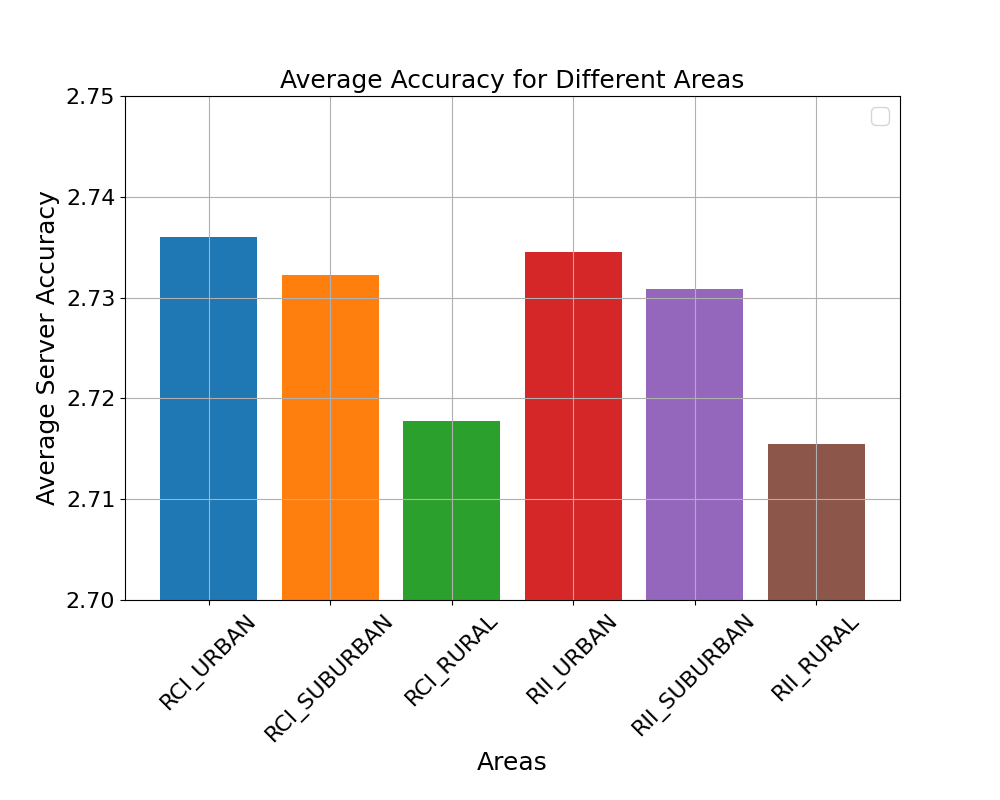
\includegraphics[width=\textwidth]{figures/chapter4/Area_Average_Accuracy.png}
    \caption{Ακρίβεια Εξυπηρετητών Μετανοητικής Μάθησης σε διαφορετικές περιοχές}
    \label{fig21}
\end{figure}

\begin{figure}[H]
    \centering
    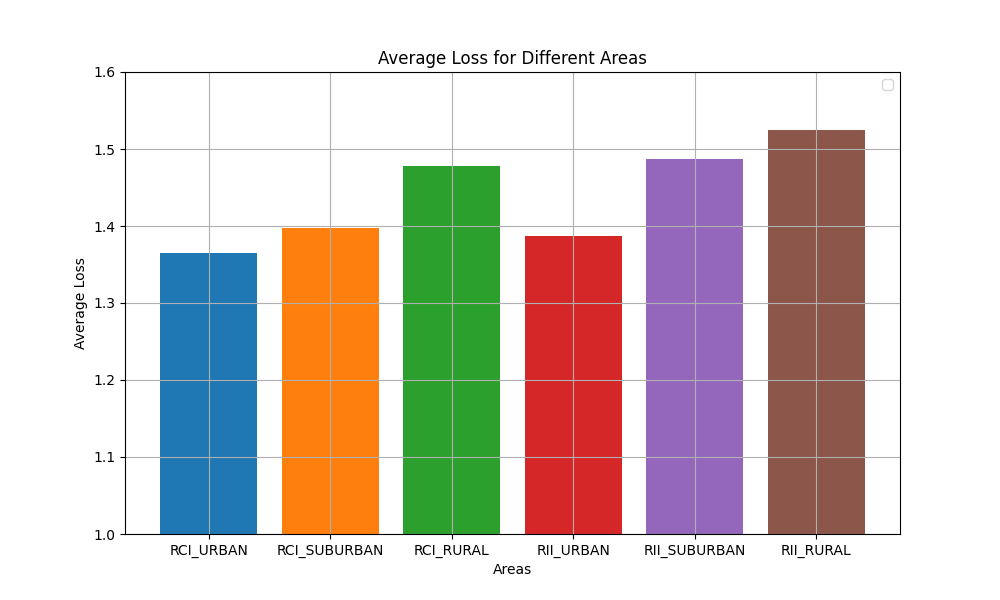
\includegraphics[width=\textwidth]{figures/chapter4/Area_of_Average_Loss.png}
    \caption{Απώλεια Εξυπηρετητών Μετανοητικής Μάθησης σε διαφορετικές περιοχές}
    \label{fig22}
\end{figure}

\newpage

Όπως βλέπουμε στα παραπάνω σχήματα \ref{fig21} και \ref{fig22} υπάρχουν διαφοροποιήσεις στις επιδόσεις της Ομοσπονδιακής Μάθησης ανάλογα με τον αλγόριθμο που χρησιμοποιείται για την αντιστοίχιση και διαμόρφωση των κόμβων, αλλά και ανάλογα με την περιοχή στην οποία βρισκόμαστε. Έτσι, για τον αλγόριθμο Πλήρους Πληροφορίας, όπου βρίσκονται κατά βάση οι βέλτιστες λύσεις, παρατηρούμε πως πετυχαίνουμε την μικρότερη απώλεια στην Αστική Περιοχή, έπειτα στα Προάστια και τέλος στην Αγοριτκή Περιοχή, όπως είναι και το αναμενόμενο. Από την άλλη πλευρά, στον αλγόριθμο Ελλιπούς Πληροφορίας βλέπουμε μια απόκλιση στην Αστική Περιοχή που δεν συμβαδίζει με το προηγούμενο συμπέρασμα. Στον αλγόριθμο αυτό όμως δεν βρίσκουμε πάντα τις βέλτιστες λύσεις, λόγω απώλειας πλήρους πληροφορίας, και άρα οι τελικές αποφάσεις των κόμβων μπορεί να διαθέτουν λιγότερα δεδομένα στην Ομοσπονδιακή Μάθηση από ότι στην βέλτιστη λύση της Πλήρους Πληροφορίας.

\newpage

\section{Σύγκριση Μετανοητικής Μάθησης με Θεωρία Παιγνίων}

Επίσης, σημαντική πληροφορία παίρνουμε συγκρίνοντας τους δύο αλγορίθμους Μετανοητικής Μάθησης μεταξύ τους, αλλά και με τον αλγόριθμο του κεφαλαίου 2. Στο σημείο αυτό θα δούμε τα πλεονεκτήματα και μειονεκτήματα του κάθε αλγορίθμου και την επίδοσή του σε διαφορετικές περιπτώσεις. Όσον αφορά τα φυσικά μεγέθη τα οποία μελετάμε για τους κόμβους μας παρατηρούμε τα εξής:

\begin{figure}[H]
    \centering
    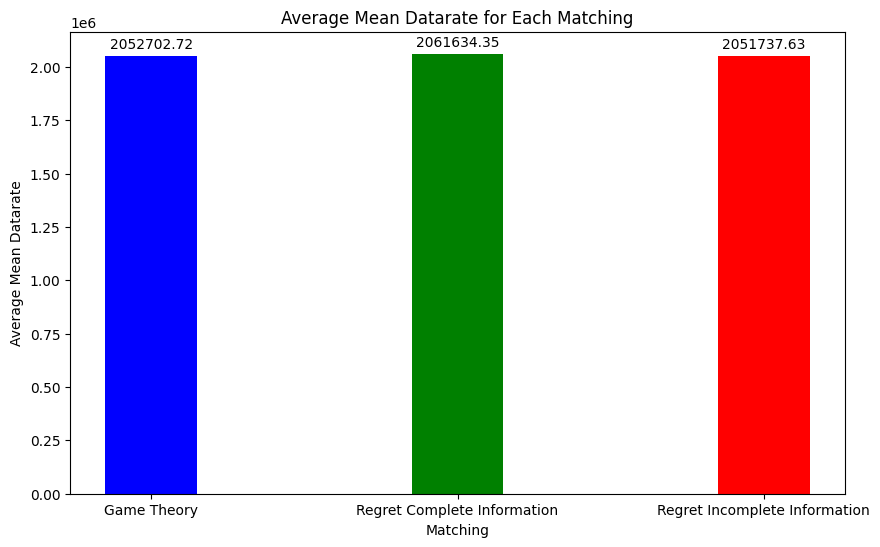
\includegraphics[width=0.85\textwidth]{figures/chapter4/Average_Mean_Datarate.png}
    \caption{Μέση ροή δεδομένων για τους κόμβους ανά αλγόριθμο αντιστοίχισης}
    \label{fig23}
\end{figure}

\begin{figure}[H]
    \centering
    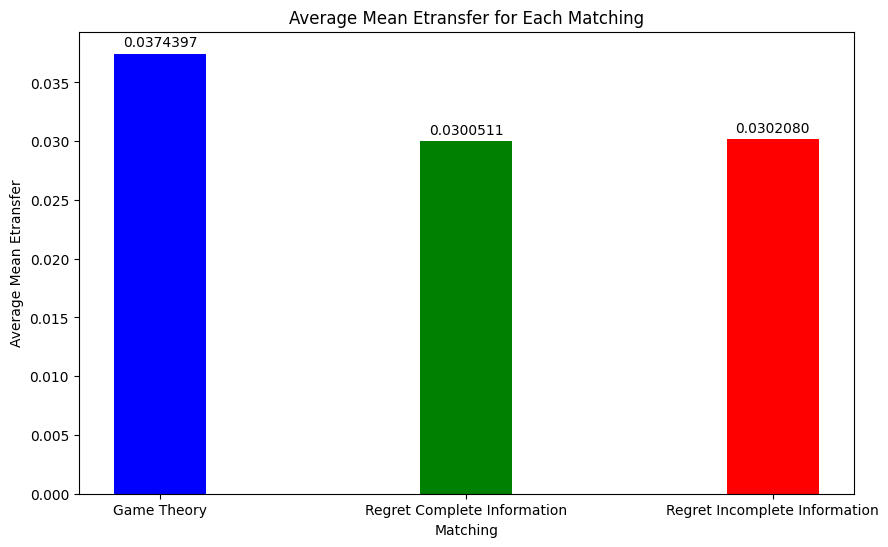
\includegraphics[width=0.85\textwidth]{figures/chapter4/Average_Mean_Etransfer.png}
    \caption{Μέση ενέργεια μετάδοσης για τους κόμβους ανά αλγόριθμο αντιστοίχισης}
    \label{fig24}
\end{figure}

\newpage

\begin{figure}[H]
    \centering
    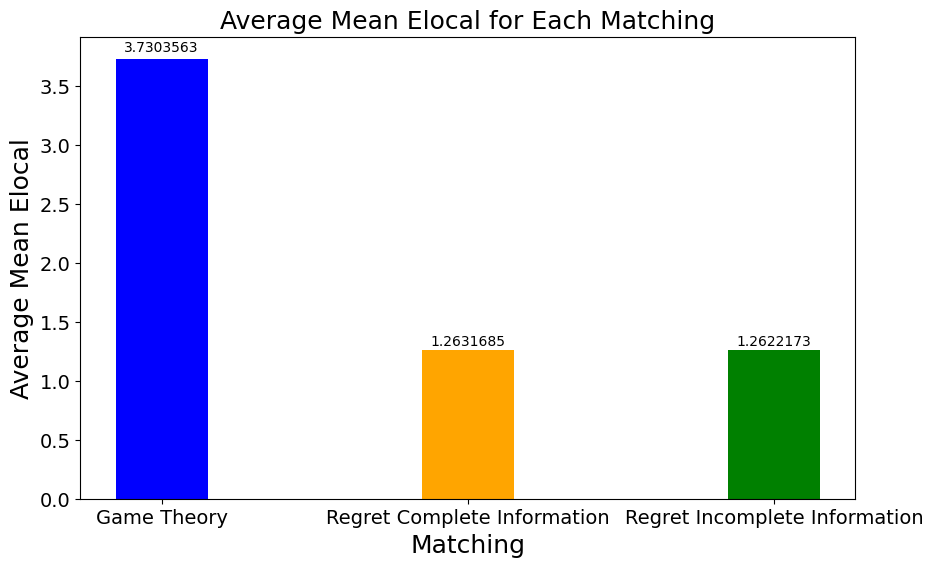
\includegraphics[width=0.85\textwidth]{figures/chapter4/Average_Mean_Elocal.png}
    \caption{Μέση ενέργεια εκπαίδευσης για τους κόμβους ανά αλγόριθμο αντιστοίχισης}
    \label{fig25}
\end{figure}

\begin{figure}[H]
    \centering
    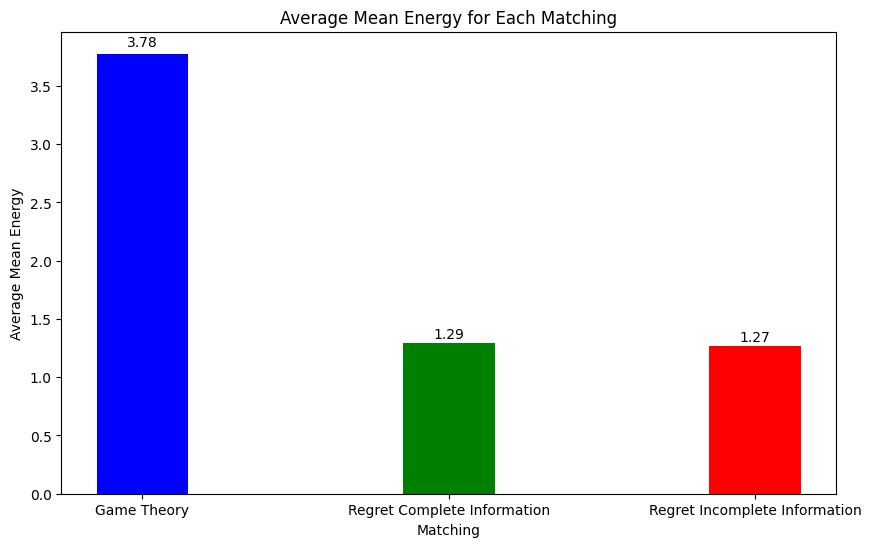
\includegraphics[width=0.85\textwidth]{figures/chapter4/Average_Mean_Energy.png}
    \caption{Μέση συνολική ενέργεια για τους κόμβους ανά αλγόριθμο αντιστοίχισης}
    \label{fig26}
\end{figure}

Αρχικά, όπως βλέπουμε στα παραπάνω διαγράμματα (\ref{fig23}, \ref{fig24}, \ref{fig25}, \ref{fig26}) οι αλγόριθμοι Μετανοητικής Μάθησης μας δίνουν πολύ καλύτερα αποτελέσματα, ειδικά σε εξοικονόμηση ενέργειας (είτε μετάδοσης, είτε εκπαίδευσης), πετυχαίνοντας παράλληλα καλύτερη μέση ροή μετάδοσης δεδομένων. Αυτό είναι λογικό, αφού οι δύο αλγόριθμοι δίνουν την δυνατότητα στους κόμβους να μεταβάλλουν τους πόρους που διαθέτουν στο σύστημά μας. Έτσι κάποιος πιο απομακρισμένος κόμβος δεν "αναγκάζεται" να χρησιμοποιήσει όλους τους πόρους του καταναλώνοντας παραπάνω ενέργεια για μικρό κέρδος, ενώ αντίστοιχα σε ανταγωνιστικά μεγέθη όπως η Ροή Δεδομένων, ελευθερώνονται πόροι του συστήματος για τους πιο ενεργούς - σημαντικούς κόμβους. Από τους δύο αλγορίθμους Μετανοητικής Μάθησης, καλύτερα αποτελέσματα μας δίνει προφανώς ο αλγόριθμος Πλήρους Πληροφορίας, ο οποίος εξετάζει αναλυτικά την συμπεριφορά όλων των πιθανών ενεργειών του κάθε κόμβου παίρνοντας υπόψη και τις ενέργειες των υπολοίπων. Αυτό μπορεί να μην είναι προφανές για την ώρα, αφού όπως βλέπουμε στα διαγράμματα \ref{fig19} και \ref{fig20}, ο αλγόριθμος Ελλιπούς Πληροφορίας πετυχαίνει χαμηλότερη κατανάλωση ενέργειας από ότι ο Πλήρους Πληροφορίας.

\begin{figure}[H]
    \centering
    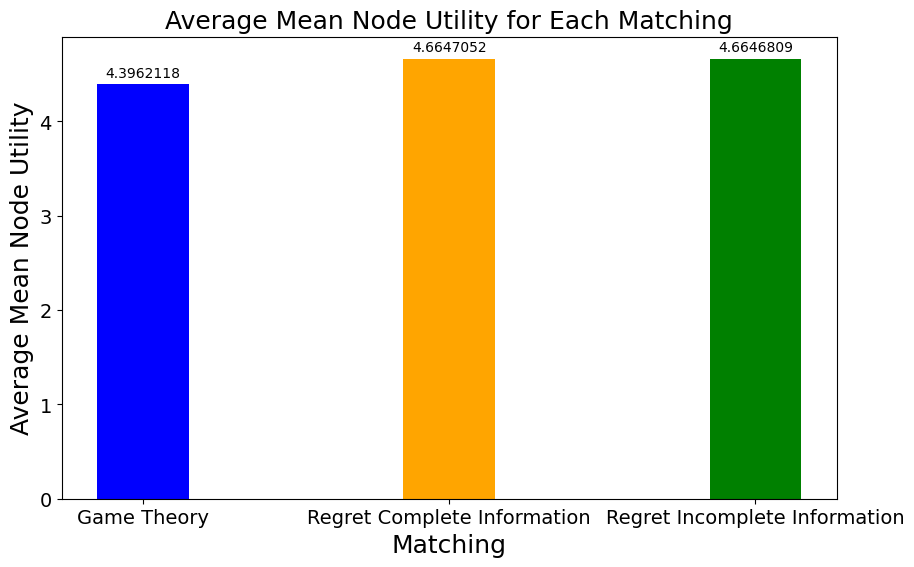
\includegraphics[width=0.85\textwidth]{figures/chapter4/Average_Mean_User_Utility.png}
    \caption{Μέση χρησιμότητα κόμβων ανά αλγόριθμο αντιστοίχισης}
    \label{fig27}
\end{figure}

\begin{figure}[H]
    \centering
    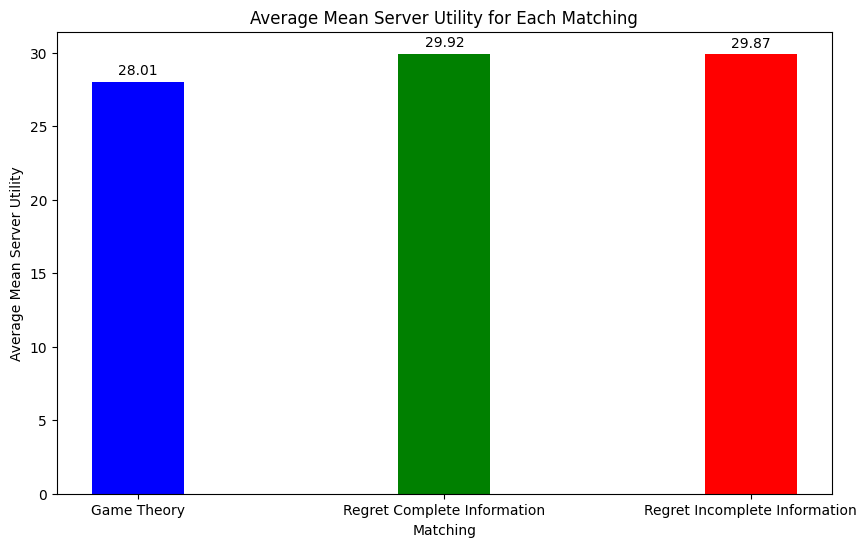
\includegraphics[width=0.85\textwidth]{figures/chapter4/Average_Mean_Server_Utility.png}
    \caption{Μέση χρησιμότητα εξυπηρετητών ανά αλγόριθμο αντιστοίχισης}
    \label{fig28}
\end{figure}

\newpage

Έτσι, στα διαγράμματα \ref{fig27} και \ref{fig28}, όπου απεικονίζεται η μέση χρησιμότητα που επιτυγχάνουν οι κόμβους και οι εξυπηρετητές, γίνεται εμφανές πλέον πως ο αλγόριθμος Πλήρους Πληροφορίας πετυχαίνει καλύτερα αποτελέσματα από τον αλγόριθμο Ελλιπούς Πληροφορίας, αφού εν τέλει η μετρική με την οποία παίρνονται οι αποφάσεις στον εκάστοτε αλγόριθμο είναι η χρησιμότητα. 

Παρολαυτά ο αλγόριθμος Πλήρους Πληροφορίας έχει και κάποια μειονεκτήματα, συγκεκριμένα στον χρόνο που απαιτεί για να επιτύχει σύγκλιση. Πιο αναλυτικά βλέπουμε:

\begin{figure}[H]
    \centering
    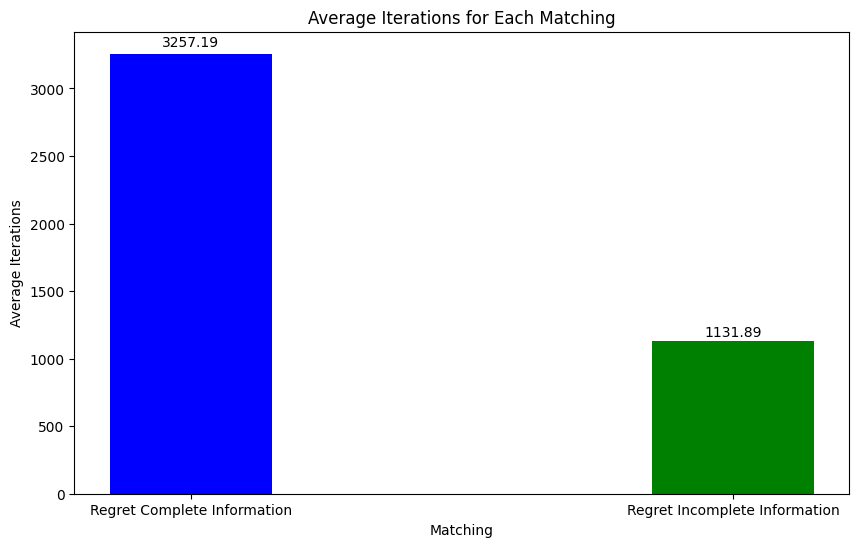
\includegraphics[width=0.85\textwidth]{figures/chapter4/Average_Iterations.png}
    \caption{Μέσος αριθμός επαναλήψεων ανά αλγόριθμο αντιστοίχισης}
    \label{fig29}
\end{figure}

\begin{figure}[H]
    \centering
    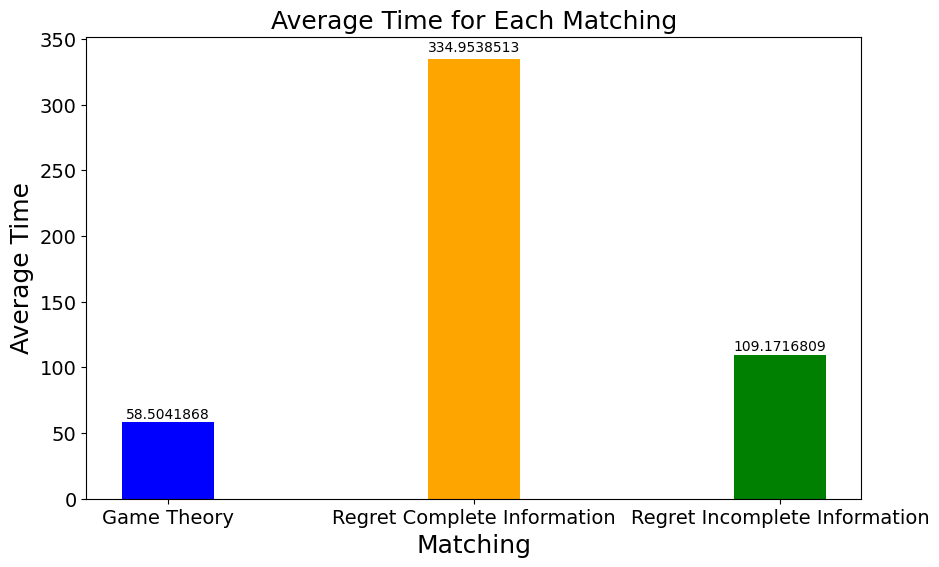
\includegraphics[width=0.85\textwidth]{figures/chapter4/Average_Time.png}
    \caption{Μέσος χρόνος εκτέλεσης ανά αλγόριθμο αντιστοίχισης}
    \label{fig30}
\end{figure}

Άρα παρότι εν γένει παίρνουμε καλύτερα αποτελέσματα με τον αλγόριθμο Πλήρους Πληροφορίας, έχει ένα μεγάλο μειονέκτημα στον μεγάλο χρόνο που απαιτεί για την εκτέλεσή του (\ref{fig30}). Αυτό θα μπορούσε να είναι ένα κρίσιμο σημείο για συχνά μεταβαλλόμενα συστήματα, στα οποία απαιτείται συχνή επαναπροσαρμογή των παικτών. Αντίστοιχα, έχουμε μεγαλύτερο αριθμό επαναλήψεων στον αλγόριθμο Πλήρους Πληροφορίας (\ref{fig29}), διότι, ειδικά σε περιπτώσεις περισσότερων κόμβων, η επιρροή μεταξύ των κόμβων στην τελική τους απόφαση καθιστά πιο δύσκολη τη σύγκλιση. Αυτό συμβαίνει, αφού για τα εξωτερικά επηρεαζόμενα μεγέθη των κόμβων, οι συνθήκες είναι ευμεταύλητες μέχρι να αρχίσουμε να οδεύουμε προς την σύγκλιση όλων των κόμβων.

\begin{figure}[H]
    \centering
    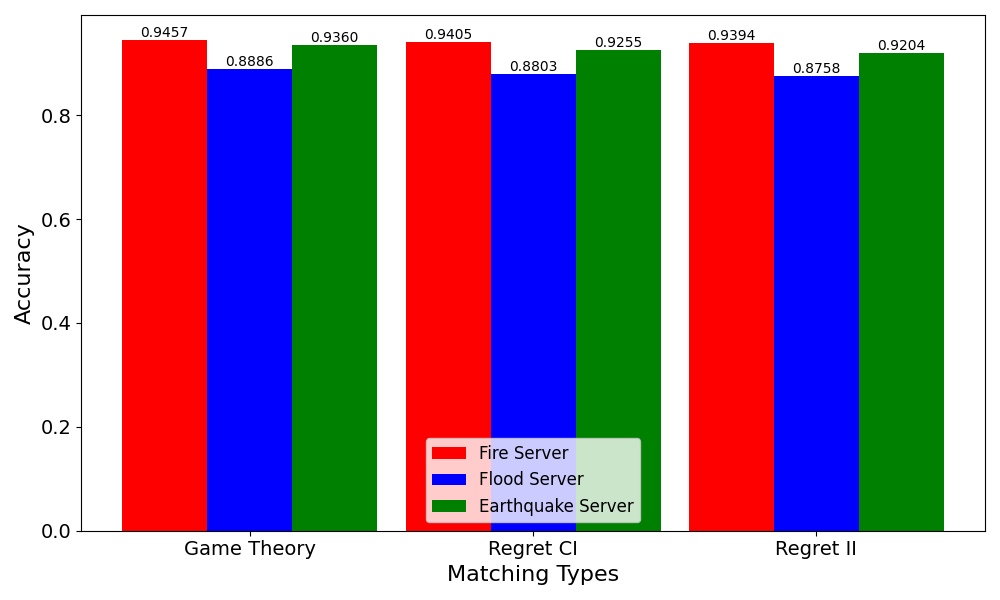
\includegraphics[width=0.9\textwidth]{figures/chapter4/accuracy_plot.png}
    \caption{Ακρίβεια Εξυπηρετητών ανά αλγόριθμο αντιστοίχισης}
    \label{fig31}
\end{figure}

\begin{figure}[H]
    \centering
    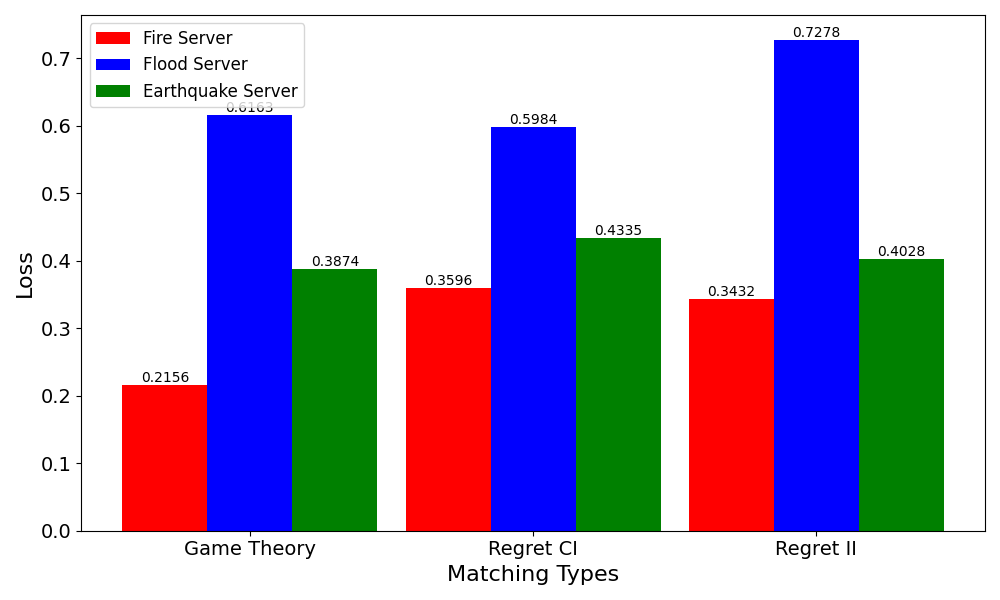
\includegraphics[width=0.9\textwidth]{figures/chapter4/loss_plot.png}
    \caption{Απώλεια Εξυπηρετητών ανά αλγόριθμο αντιστοίχισης}
    \label{fig32}
\end{figure}

\newpage

Στο κομμάτι της Ομοσπονδιακής Μάθησης παρατηρούμε πως ανάλογα με την σημασία κάθε κόμβου και τις απολαβές που μπορεί να συλλέξει, στους αλγορίθμους Μετανοητικής Μάθησης, ο κόμβος μπορεί να επιλέξει να διαθέσει λιγότερα δεδομένα στην διαδικασία της εκμάθησης. Αυτό έχει ως αποτέλεσμα, όπως φαίνεται στα \ref{fig31} και \ref{fig32}, να πετυχαίνουμε χειρότερα αποτελέσματα στην εκπαίδευση των μοντέλων με τους δύο αυτούς αλγορίθμους. Από την άλλη πλευρά, βλέπουμε πως και οι δύο αλγόριθμοι Μετανοητικής Μάθησης φτάνουν αρκετά κοντά σε επιδόσεις συγκριτικά με τον αλγόριθμο Θεωρίας Παιγνίων. Δεδομένου ότι πετυχαίνουμε αυτό το αποτέλεσμα, με τα μικρότερα σύνολα δεδομένων που χρησιμοποιούν οι αλγόριθμοι Μετανοητικής Μάθησης, είναι εμφανές πως το μοντέλο μας σε συνδυασμό με μια ορθή αντιστοίχιση και διαμόρφωση των κόμβων πετυχαίνει πολύ καλές επιδόσεις.

Αντίστοιχα, είναι σημαντικό να μελετήσουμε και την συμπεριφορά των αλγορίθμων μας ανάλογα με το μέγεθος των κόμβων που καλούνται να διαχειριστούν.

\begin{figure}[ht]
    \centering
    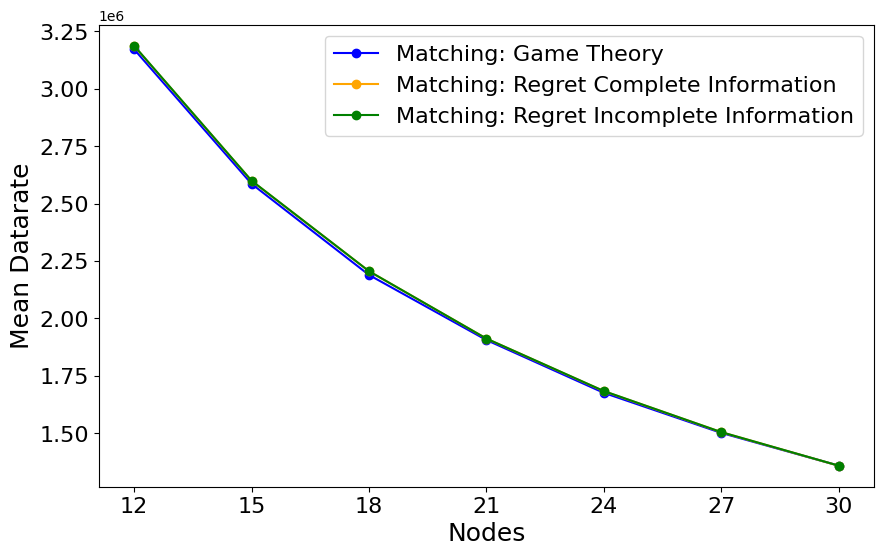
\includegraphics[width=\textwidth]{figures/chapter4/Mean_Datarate_vs_Users.png}
    \caption{Μέση ροή δεδομένων ανά αριθμό κόμβων ανά αλγόριθμο αντιστοίχισης}
    \label{fig33}
\end{figure}

Αρχικά, όπως είδαμε και παραπάνω, επαναλαμβάνεται η επικράτηση των αλγορίθμων Μετανοητικής Μάθησης σε σχέση με τον αλγόριθμος Θεωρίας Παιγνίων, λόγω της δυνατότητάς που τους έχουμε δώσει να διαμορφώνουν τη συμπεριφορά του κάθε κόμβου (\ref{fig33}, \ref{fig34}, \ref{fig35}, \ref{fig36}). Βλέπουμε πως η μέση ροή δεδομένων μειώνεται όσο ο αριθμός των κόμβων αυξάνεται (\ref{fig33}), το οποίο είναι λογικό, αφού οι κόμβους μας μοιράζονται το κοινό εύρος ζώνης που διαθέτει ο εξυπηρετητής για την επικοινωνία με αυτούς. Όλοι οι αλγόριθμοι διατηρούν περίπου όμοια κλιμάκωση ανάλογα με τον αριθμό των κόμβων, με τον αλγόριθμο Πλήρους Πληροφορίας να πετυχαίνει το καλύτερο αποτέλεσμα, ακολουθούμενο από τον αλγόριθμο Ελλιπούς Πληροφορίας και τέλος από τον αλγόριθμο Θεωρίας Παιγνίων, εξαιρώντας την περίπτωση των 30 κόμβων, όπου επειδή όσο μικρότερης σημασίας είναι οι κόμβους τόσο μικρότερο εύρος ζώνης διεκδηκούν (\ref{eq25} και \ref{eq26}) και άρα ρίχνουν τον μέσο όρο. 

\begin{figure}[ht]
    \centering
    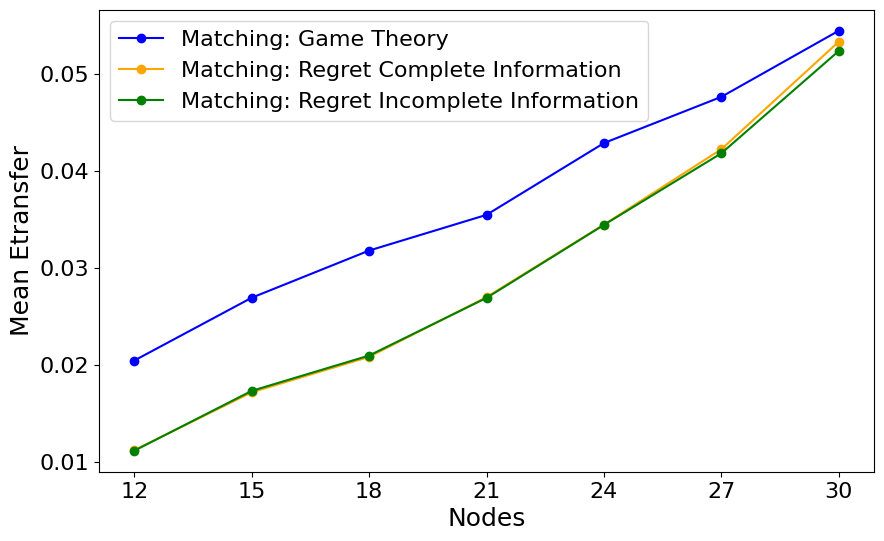
\includegraphics[width=\textwidth]{figures/chapter4/Mean_Etransfer_vs_Users.png}
    \caption{Μέση ενέργεια μετάδοσης ανά αριθμό κόμβων ανά αλγόριθμο αντιστοίχισης}
    \label{fig34}
\end{figure}

Και για τους τρεις αλγορίθμους η μέση ενέργεια μετάδοσης αυξάνεται όσο αυξάνεται και ο αριθμός των κόμβων (\ref{fig34}). Η συμπεριφορά αυτή είναι προϊόν του ανταγωνισμού, όπως είδαμε και στη ροή δεδομένων. Οι κόμβους ανταγωνίζονται για πόρους και άρα προσπαθούν να διαθέσουν παραπάνω ισχύ, και άρα και ενέργεια, με σκοπό να διεκδηκήσουν τους πόρους αυτούς. Συγκεκριμένα, όπως βλέπουμε και στο \ref{fig34} η ενέργεια μετάδοσης για τους αλγορίθμους Μετανοητικής Μάθησης αυξάνεται με μεγαλύτερο ρυθμό, ενώ συγκεκριμένα για 30 κόμβους η ενέργεια που καταναλώνεται από τους κόμβους είναι μεγαλύτερη από αυτή στον αλγόριθμο της Θεωρίας Παιγνίων. Αυτό συμβαίνει επειδή όλοι οι κόμβους μεταδίδουν τον ίδιο αριθμό δεδομένων στον κεντρικό εξυπηρετητή, οι πιο απομακρισμένοι, διεκδηκώντας μικρότερο εύρος ζώνης θα απαιτούν περισσότερη ώρα για να μεταδόσουν την πληροφορία και άρα θα έχουν μεγαλύτερη κατανάλωση ενέργειας.

Όπως βλέπουμε στο σχ.\ref{fig35}, καθώς ο αριθμός των κόμβων αυξάνεται, ο μέσος όρος της ενέργειας εκπαίδευσης σε κάθε περίπτωση μειώνεται. Αυτό συμβαίνει, διότι οι πιο απομακρισμένοι κόμβους έχουν στη διάθεσή του μικρότερα σύνολα δεδομένων, αφού βρίσκονται πιο μακριά από τα κρίσιμα σημεία. Αντίστοιχα, επειδή οι αλγόριθμοι Μετανοητικής Μάθησης έχουν την δυνατότητα προσαρμογής του συνόλου δεδομένου που προσφέρει ο κάθε κόμβος στην Ομοσπονδιακή Μάθηση, επιτυγχάνουν πολύ μικρότερη μέση κατανάλωση ενέργειας εκπαίδευσης. 

\newpage

\begin{figure}[H]
    \centering
    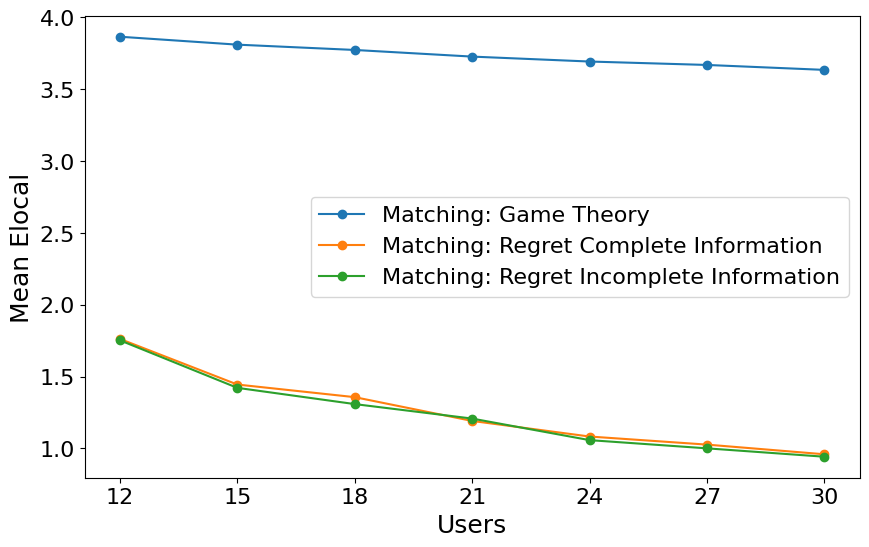
\includegraphics[width=\textwidth]{figures/chapter4/Mean_Elocal_vs_Users.png}
    \caption{Μέση ενέργεια εκπαίδευσης ανά αριθμό κόμβων ανά αλγόριθμο αντιστοίχισης}
    \label{fig35}
\end{figure}

\begin{figure}[H]
    \centering
    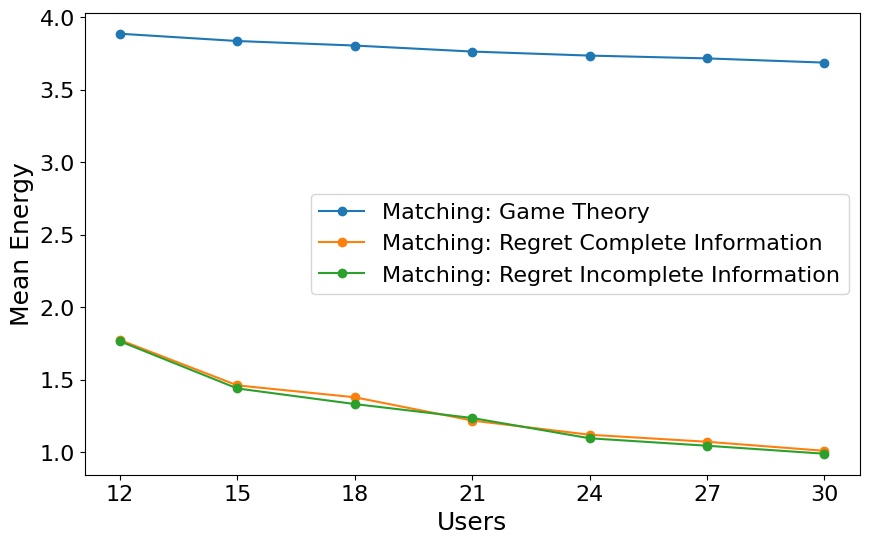
\includegraphics[width=\textwidth]{figures/chapter4/Mean_Energy_vs_Users.png}
    \caption{Μέση συνολική ενέργεια ανά αριθμό κόμβων ανά αλγόριθμο αντιστοίχισης}
    \label{fig36}
\end{figure}

\newpage

Για τον ίδιο λόγο επίσης η μέση κατανάλωση ενέργειας εκπαίδευσης μειώνεται με μεγαλύτερο ρυθμό στους αλγορίθμους Μετανοητικής Μάθησης. Στον αλγόριθμο Πλήρους Πληροφορίας βλέπουμε πως γενικά έχουμε μια μεγαλύτερη κατανάλωση ενέργειας, όπου όπως είδαμε και προηγουμένως είναι λόγω της καλύτερης αξιοποίησης των συνόλων δεδομένων των κόμβων. Αντίστοιχα, στο σχ.\ref{fig36} βλέπουμε πως η μέση συνολική ενέργεια παρουσιάζει αντίστοιχη μορφή με την μέση ενέργεια εκπαίδευσης, αφού το μεγαλύτερο μέρος της ενέργειας που καταναλώνεται αφορά την τοπική εκπαίδευση για κάθε κόμβου.

\begin{figure}[H]
    \centering
    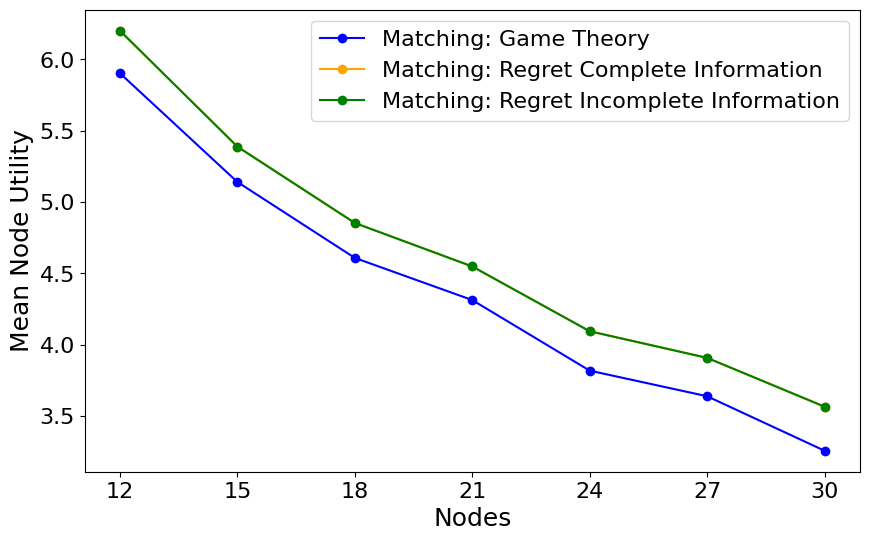
\includegraphics[width=0.8\textwidth]{figures/chapter4/Mean_User_Utility_vs_Users.png}
    \caption{Μέση χρησιμότητα κόμβων ανά αριθμό κόμβων ανά αλγόριθμο αντιστοίχισης}
    \label{fig37}
\end{figure}

\begin{figure}[H]
    \centering
    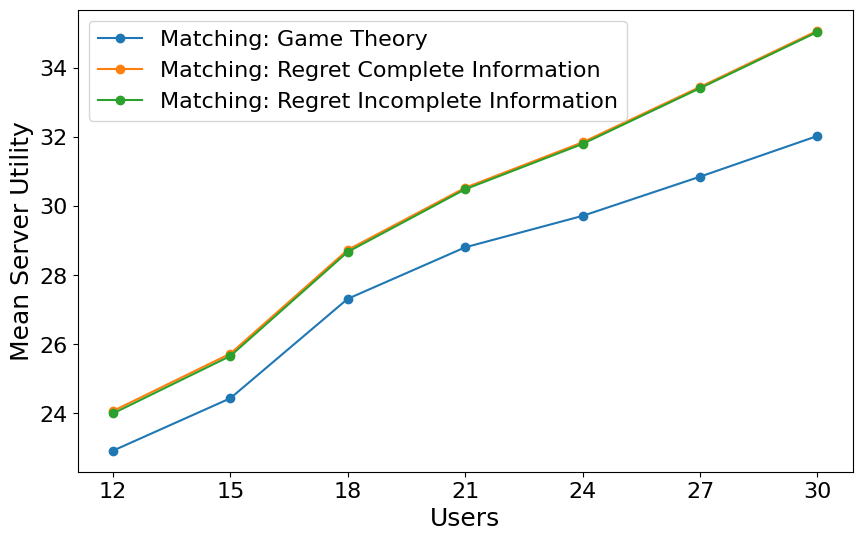
\includegraphics[width=0.8\textwidth]{figures/chapter4/Mean_Server_Utility_vs_Users.png}
    \caption{Μέση χρησιμότητα εξυπηρετητών ανά αριθμό κόμβων ανά αλγόριθμο αντιστοίχισης}
    \label{fig38}
\end{figure}

\newpage

Όπως βλέπουμε στο σχ.\ref{fig37} η μέση χρησιμότητα των κόμβων πέφτει όσο περισσότεροι κόμβους ζουν στο σύστημά μας. Αυτό είναι λογικό, αφού με περισσότερους κόμβους έχουμε και μεγαλύτερο ανταγωνισμό για τους μοιραζόμενους πόρους, ενώ παράλληλα οι νέοι κόμβους, όντας πιο μακρινοί από τα κρίσιμα σημεία, είναι μικρότερης σημασίας και άρα έχουν μικρότερες μέγιστες τιμές χρησιμότητας, ρίχνοντας το μέσο όρο. Αυτό φαίνεται αντίστοιχα στο σχ.\ref{fig38}, όπου όσο περισσότεροι κόμβους είναι διαθέσιμοι, τόσο λιγότερο κλιμακώνει η χρησιμότητα των εξυπηρετητών. Επιπλέον, η χρησιμότητα των εξυπηρετητών αυξάνεται με την αύξηση των κόμβων, αφού περισσότεροι κόμβους προσφέρουν σε κάθε εξυπηρετητή.

Όσον αφορά τον χρόνο εκτέλεσης και τον αριθμό επαναλήψεων που απαιτεί κάθε αλγόριθμος (σχ.\ref{fig39} και σχ.\ref{fig40}) μπορούμε να δούμε πως ο αλγόριθμος Πλήρους Πληροφορίας αυξάνει πολύ σε υπολογιστικό κόστος πολύ γρήγορα σε σχέση με τον αριθμό των κόμβων. Αντίθετα, ο Ελλιπούς Πληροφορίας παρουσιάζει ίδιο κόστος και σε επαναλήψεις και σε χρόνο, ανεξαιρέτως του πλήθους των κόμβων καθιστώντας τον μη ιδανικό για μικρά Ν, αλλά δίνοντάς του πολύ καλή κλιμάκωση.  Τέλος ο αλγόριθμος Θεωρίας Παιγνίων αυξάνει αργά σε υπολογιστικό κόστος, με γραμμικό τρόπο. Για τους δύο αλγορίθμους Μετανοητικής Μάθησης μπορούμε να παρατηρήσουμε επίσης το εξής. Ο αλγόριθμος Ελλιπούς Πληροφορίας φαίνεται να συγκλίνει ανεξάρτητα του αριθμού των κόμβων και της θέσης τους, καθιστώντας τον ιδανικό για παντώς είδους συστήματα, ενώ το φθηνό υπολογιστικό του κόστος τον καθιστά πολύ γρήγορο στην εκτέλεση. Αντίθετα φαίνεται ο αλγόριθμος Πλήρους Πληροφορίας να επηρεάζεται στην σύγκλιση και άρα και στον χρόνο εκτέλεσης από την θέση των εκάστοτε κόμβων, αφού αν δούμε οι μεγάλες διαφοροποιήσεις στον χρόνο εκτέλεσης και στον αριθμό επαναλήψεων συμβαίνουν στους 12 και 21 κόμβους που αποτελούν και τα δύο όρια για τις διαφορετικές περιοχές μας.

\begin{figure}[H]
    \centering
    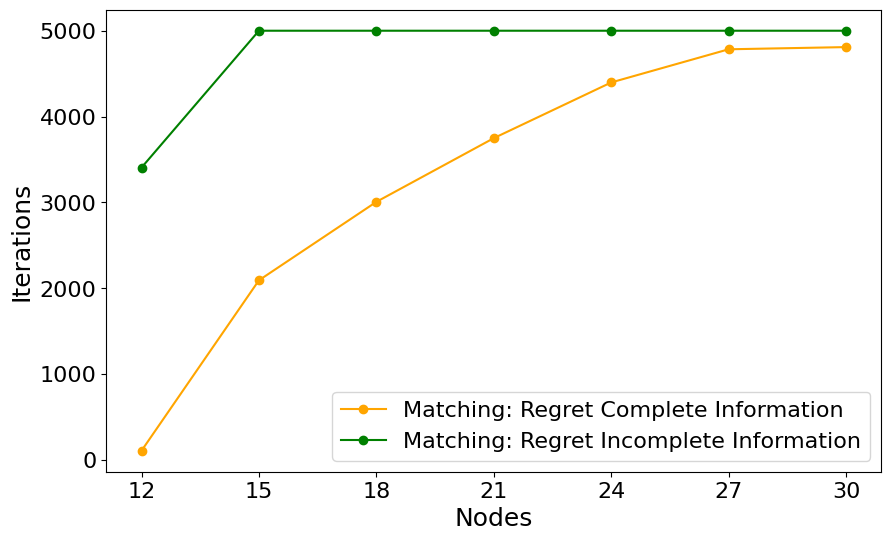
\includegraphics[width=\textwidth]{figures/chapter4/Iterations_vs_Users.png}
    \caption{Μέσος αριθμός επαναλήψεων ανά αριθμό κόμβων ανά αλγόριθμο αντιστοίχισης}
    \label{fig39}
\end{figure}

\newpage

\begin{figure}[H]
    \centering
    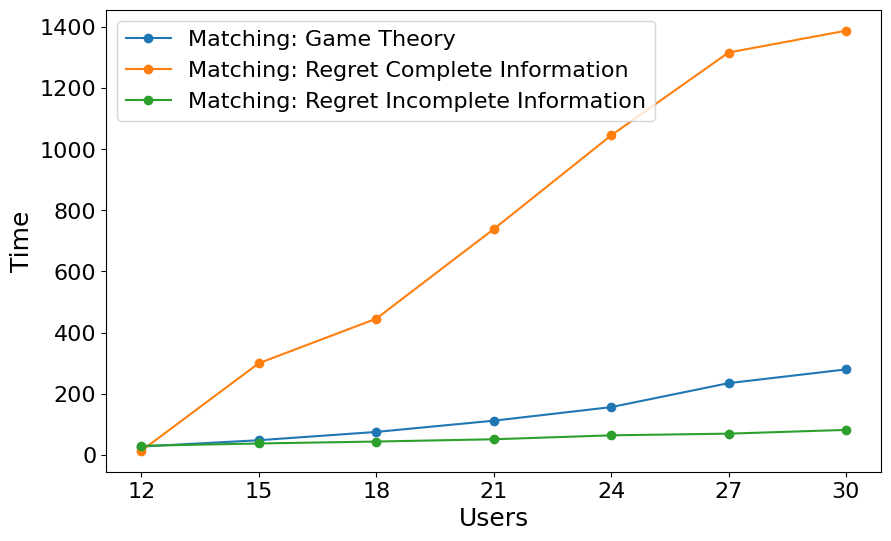
\includegraphics[width=\textwidth]{figures/chapter4/Time_vs_Users.png}
    \caption{Μέσος χρόνος εκτέλεσης ανά αριθμό κόμβων ανά αλγόριθμο αντιστοίχισης}
    \label{fig40}
\end{figure}

Μελετώντας παραπάνω αυτή τη συμπεριφορά βλέπουμε:

\begin{figure}[H]
    \centering
    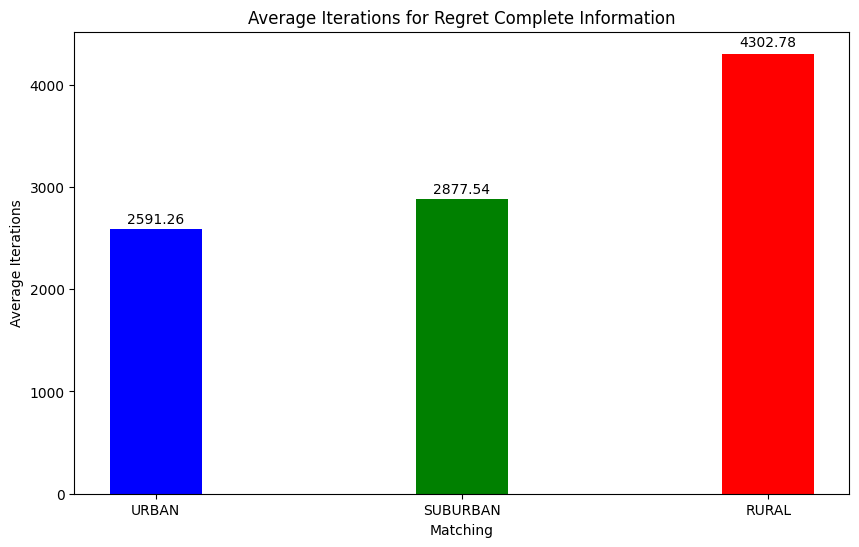
\includegraphics[width=\textwidth]{figures/chapter4/Average_Iterations_per_area_RCI.png}
    \caption{Επαναλήψεις Αλγορίθμου Πλήρους Πληροφορίας ανά Περιοχή}
    \label{fig41}
\end{figure}

\newpage

\begin{figure}[H]
    \centering
    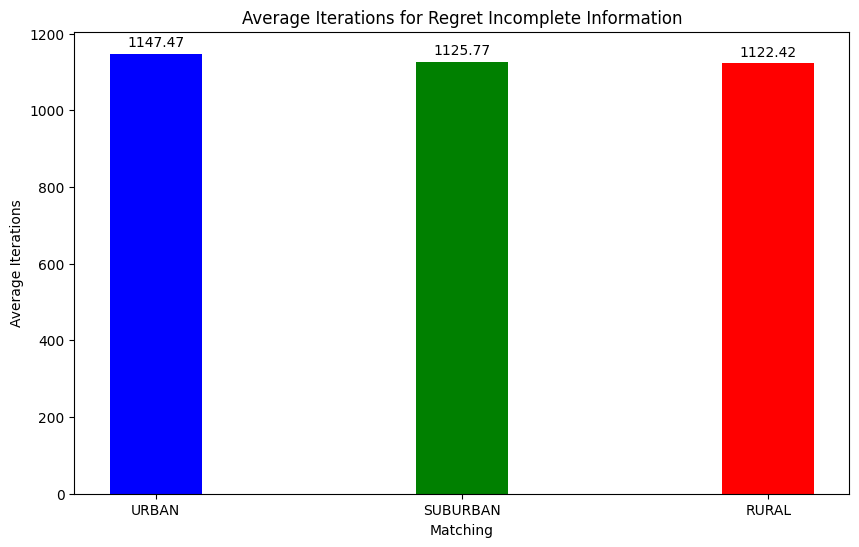
\includegraphics[width=\textwidth]{figures/chapter4/Average_Iterations_per_area_RII.png}
    \caption{Επαναλήψεις Αλγορίθμου Ελλιπούς Πληροφορίας ανά Περιοχή}
    \label{fig42}
\end{figure}

\begin{figure}[H]
    \centering
    \includegraphics[width=\textwidth]{figures/chapter4/Average_Time_per_area_RCI.png}
    \caption{Χρόνος Εκτέλεσης Αλγορίθμου Πλήρους Πληροφορίας ανά Περιοχή}
    \label{fig43}
\end{figure}

\begin{figure}[H]
    \centering
    \includegraphics[width=\textwidth]{figures/chapter4/Average_Time_per_area_RII.png}
    \caption{Χρόνος Εκτέλεσης Αλγορίθμου Ελλιπούς Πληροφορίας ανά Περιοχή}
    \label{fig44}
\end{figure}

Στα σχήματα \ref{fig41} και \ref{fig42} γίνεται εμφανής η παρατήρηση που κάναμε παραπάνω. Όσο πιο πολλοί απομακρισμένοι κόμβους ζουν στο σύστημά μας τόσο περισσότερο δυσκολεύεται να φτάσει σε σύγκλιση ο αλγόριθμος Πλήρους Πληροφορίας σε αντίθεση με τον Ελλιπούς Πληροφορίας. Αντίστοιχα αυτό μας οδηγεί στα διαγράμματα \ref{fig43} και \ref{fig44}, όπου αντίστοιχα με τον αριθμό των επαναλήψεων του αλγορίθμου έχουμε και διαμόρφωση των χρόνων εκτέλεσης. Η διαφοροποιήση αυτή στους δύο αλγορίθμους συμβαίνει, διότι όσο πιο μακρινούς κόμβους έχουμε, τόσο πιο δύσκολη είναι η σύγκλιση στον αλγόριθμο Πλήρους Πληροφορίας στην βέλτιστη διαμόρφωση του κόμβου, διότι αυτή κατά πάσα πιθανότητα διαφέρει από άλλες κατά πολύ λίγο και συνεπώς, οι μετάνοιες για τις κοντινές αυτές πράξεις μειώνονται με πολύ αργό ρυθμό. Αντίθετα, στον αλγόριθμο Ελλιπούς Πληροφορίας η αρχικοποίηση των χρησιμοτήτων, σε συνδυασμό με το γεγονός πως σε κάθε επανάληψη δεν ενημερώνονται όλες οι χρησιμότητες, αλλά και λόγω του λευκού θορύβου που δημιουργεί μεγαλύτερες διαφορές στις χρησιμότητες, επιτυγχάνουμε πιο γρήγορη σύγκλιση.

\newpage

\begin{figure}[ht]
    \centering
    \includegraphics[width=\textwidth]{figures/chapter4/RCI_Iterations_vs_Users_per_Area.png}
    \caption{Μέσος αριθμός επαναλήψεων ανά αριθμό κόμβων ανά περιοχή}
    \label{fig45}
\end{figure}

Στο διάγραμμα \ref{fig45} βλέπουμε πιο αναλυτικά την διακύμανση των απαιτούμενων επαναλήψεων για τον αλγόριθμο Πλήρους Πληροφορίας, ανά περιοχή, όσο αυξάνεται ο αριθμός των κόμβων. Είναι εμφανές, πως όταν αρχίσουν σε κάθε περιοχή να εισέρχονται πιο απομακρισμένοι κόμβους, η σύγκλιση δυσχαιρένει. Αντίστοιχα, όσο περισσότεροι κόμβους υπάρχουν στο σύστημά μας, τόσο πιο δύσκολη γίνεται η σύγκλιση, αφού κατ' αρχήν θέλουμε όλοι μας οι κόμβους να συγκλίνουν, ενώ επιπλέον, αφού το περιβάλλον μας είναι ανταγωνιστικό, οι αλλαγές συμπεριφοράς ενός κόμβου είναι πιθανό να επηρεάσουν και τους υπολοίπους στη βέλτιστη επιλογή τους.
\chapter{Συμπεράσματα}

Έπειτα από μελέτη των διαφόρων σεναρίων, αλγορίθμων και αποτελεσμάτων μπορούμε να καταλήξουμε σε κάποια γενικά συμπεράσματα από την διαδικασία αυτής της διπλωματικής εργασίας.

Η Ομοσπονδιακή Μάθηση είναι ένας μηχανισμός που μας επιτρέπει να εξάγουμε πληροφορία από δεδομένα, χωρίς να αποκτούμε συνολική πρόσβαση σε αυτά. Έτσι διασφαλίζουμε την ιδιωτικότητα, που είναι απαραίτητη ιδιαίτερα σε συγκεκριμένους τομείς, πετυχαίνοντας παράλληλα την εκπαίδευση των μοντέλων που χρειαζόμαστε. Στην περίπτωσή μας, είχαμε τρία μοντέλα, τα οποία εκπαιδεύονταν από τους κόμβους του περιβάλλοντός μας. Ο κάθε ένας κόμβος διέθετε μια συγκεκριμένη ποσότητα και τύπο δεδομένων και άρα θα είχε διαφορετική σημασία για κάθε μοντέλο - εξυπηρετητή. Αυτό αποδίδεται στους αλγορίθμους μας με τις συναρτήσεις χρησιμότητας. Τις συναρτήσεις αυτές φαίνεται να διαχειρίζεται καλύτερα ο αλγόριθμος Θεωρίας Παιγνίων, ο οποίος καταφέρνει να κάνει τις καλύτερες αντιστοιχίσεις, κρατώντας τις χρησιμότητες υψηλότερα από τους υπόλοιπους αλγορίθμους. Συνεπώς, είναι ευθύνη μας να χτίσουμε μία αντιπροσωπευτική συνάρτηση χρησιμότητας που να αντικατοπτρίζει ορθά το πρόβλημα και τις παραμέτρους του. 

Όπως είδαμε ακόμη και με μία σχετικά απλή συνάρτηση χρησιμότητας, ο αλγόριθμος Θεωρίας Παιγνίων προσπαθώντας να την μεγιστοποιήσει καταφέρνει να πετύχει υψηλή ροή δεδομένων, χαμηλή ενέργεια μετάδοσης και καλύτερη επίδοση στην Ομοσπονδιακή Μάθηση έναντι των υπόλοιπων αλγορίθμων αντιστοίχισης. Παρ' όλα ταύτα, και οι άλλοι αλγόριθμοι πετυχαίνουν πολύ καλά αποτελέσματα, με τον αλγόριθμο Ενισχυτικής Μάθησης να είναι κοντά ως προς τη χρησιμότητα κόμβων. Είναι επίσης σημαντικό να επαναλάβουμε πως και να γίνει κάποια μη βέλτιστη αντιστοίχιση και να υπάρχει κάποιος μη χρήσιμος κόμβος στον συνασπισμό ενός εξυπηρετητή, ο μηχανισμός της ανάθεσης βαρών για την διαδικασία της Ομοσπονδιακής Μάθησης επιτρέπει να μην επηρεαστεί ιδιαίτερα η επίδοση του συγκεντρωτικού μοντέλου. Μία επιπλέον βελτίωση θα ήταν ένας εξυπηρετητής να μην λαμβάνει υπόψη του κάποιον κόμβο ο οποίος έχει πολύ μικρό βάρος έτσι ώστε να μην καταναλώνονται πόροι για την τοπική εκπαίδευση και μετάδοση των παραμέτρων του μοντέλου. Από την άλλη πλευρά με μη βέλτιστη αντιστοίχιση δεν αξιοποιείται πληροφορία που για κάποιον άλλο εξυπηρετητή θα ήταν χρήσιμη. Έτσι, ξεχωρίζουμε την ικανότητα του αλγορίθμου Θεωρίας Παιγνίων να κάνει βέλτιστη αντιστοίχιση σχεδόν σε κάθε ένα από τα σενάρια που του ανατέθηκαν. Προφανώς ο αλγόριθμος αυτός μπορεί να εφαρμοστεί και σε περιπλοκότερα συστήματα, με περισσότερους κόμβους, εξυπηρετητές και κρίσιμα σημεία, αλλά και με πιο σύνθετες συναρτήσεις χρησιμότητας (όπως είδαμε και στο κεφάλαιο 4).

Στο κεφάλαιο 4, εξετάσαμε μία άλλη προσέγγιση στο υπάρχον πρόβλημα. Οι κόμβοι πέρα από την συσχέτισή τους με τους εξυπηρετητές, μπορούν να διαμορφώσουν την συμμετοχή τους στην διαδικασία της Ομοσπονδιακής Μάθησης. Αυτό δίνει την ευελιξία στο σύστημά μας να μεγιστοποιήσει τις συναρτήσεις χρησιμότητας περαιτέρω, επιτρέποντας σε κόμβους που είναι πιο απομακρυσμένοι ή με λιγότερη πληροφορία να συμμετέχουν λιγότερο. Το μεγάλο πλεονέκτημα των αλγορίθμων Μετανοητικής Μάθησης που εφάρμοσαν την παραπάνω στρατηγική ήταν στην μεγάλη μείωση στην ενέργεια εκπαίδευσης των τοπικών μοντέλων, το οποίο αντίστοιχα μεταφράζεται και σε μείωση του χρόνου που απαιτείται για την εκπαίδευση, αφού οι πιο απομακρυσμένοι κόμβοι τείνουν να συμμετέχουν με λιγότερα δεδομένα, εφ' όσον οι κοντινοί στα κρίσιμα σημεία κόμβοι διαθέτουν την περισσότερη και κύρια πληροφορία. Όπως είδαμε φτάνουμε αρκετά κοντά σε απόδοση στην Ομοσπονδιακή Μάθηση σε σχέση με την απόλυτη προσέγγιση του αλγορίθμου Θεωρίας Παιγνίων. Όμως πετυχαίνουμε καλύτερη χρησιμότητα, με μικρότερες ενέργειες εκπαίδευσης και μετάδοσης και μεγαλύτερη ροή δεδομένων.

Αντίστοιχα, οι δυο διαφορετικές προσεγγίσεις στην Μετανοητική Μάθηση μας δείχνουν πως δεν χρειάζεται να γνωρίζουμε τις ακριβείς συμπεριφορές όλων των κόμβων στο σύστημά μας για να πάρουμε ένα εξίσου καλό, αλλά και πολύ πιο γρήγορο αποτέλεσμα. Ο αλγόριθμος Πλήρους Πληροφορίας τείνει να κάνει καλύτερες επιλογές απ' ότι ο Ελλιπούς Πληροφορίας, αλλά εν' τέλει η διαφορά είναι αρκετά μικρή ώστε να δίνει πλεονέκτημα στον μικρό χρόνο εκτέλεσης του αλγορίθμου Ελλιπούς Πληροφορίας και στην πιο γρήγορη σύγκλισή του. Συνεπώς ο αλγόριθμος αυτός κάνει μια πολύ γρήγορη αντιστοίχιση (παίρνοντας υπόψη το πόσες διαφορετικές επιλογές υπάρχουν για τον κάθε κόμβο) και πετυχαίνει υψηλές χρησιμότητες κατά μέσο όρο μένοντας λίγο πίσω από τον Πλήρους Πληροφορίας. Όσον αφορά την Ομοσπονδιακή Μάθηση έχει την μικρότερη επίδοση, όμως μένει αξιοπρεπώς κοντά στους άλλους δύο.

Τα σενάρια που μελετήσαμε μπορούν να εφαρμοστούν αντίστοιχα και σε άλλες περιπτώσεις. Η Αστική, Προαστιακή και Αγροτική Περιοχή μπορούν να δώσουν πληροφορίες για την συμπεριφορά των μοντέλων στον πραγματικό κόσμο αλλά επιτρέπει και να μελετηθούν περιπτώσεις χρήσιμων και λιγότερο χρήσιμων κόμβων. Με την πληθώρα εφαρμογών της Ομοσπονδιακής Μάθησης ένα τέτοιο οικοσύστημα μπορεί να χρησιμοποιηθεί και με άλλα δεδομένα ή για άλλα μοντέλα. Για παράδειγμα σε σενάριο μίας Έξυπνης Πόλης, μπορεί αντί για Δημόσια Ασφάλεια (πυρκαγιές, πλημμύρες, σεισμοί) να εξετασθεί μια περίπτωση αυτόματης ρύθμισης της κυκλοφορίας στους δρόμους. Το μοντέλο που χρησιμοποιήθηκε (MobileNetV3) είναι ένα πολύ μικρό σε μέγεθος και υπολογιστική πολυπλοκότητα και άρα ιδανικό για εγκατάσταση σε οποιαδήποτε συσκευή. Επιπλέον, με την τεχνική εξαγωγής δεδομένων, το ακριβό υπολογιστικά κομμάτι ανάλυσης των εικόνων γίνεται μία μόνο φορά, επιτρέποντας φθηνές επαναλήψεις στην διαδικασία της Ομοσπονδιακής Μάθησης. Αντίστοιχα, με άλλα μοντέλα (όχι εικόνων) μπορούν να μελετηθούν άλλα φαινόμενα. Για παράδειγμα, η μελέτη του κινδύνου πυρκαγιών μέσω μετρήσεων θερμοκρασίας ή η πρόγνωση σεισμών μέσω δεδομένων από δίκτυα σεισμικής παρακολούθησης, αποτελούν δύο διαφορετικές προσεγγίσεις στο πρόβλημα το οποίο εμείς εξετάσαμε με εικόνες. Στο πλαίσιο των εικόνων - δεδομένων, προφανώς με ελάχιστες αλλαγές μπορούν να δοκιμασθούν και άλλα μοντέλα, όπως τα μοντέλα EfficientNet. Ανάλογα την εφαρμογή μπορεί να κάνουν καλύτερη εξαγωγή χαρακτηριστικών από τις εικόνες και αξίζει να γίνει μελέτη για την κατάλληλη επιλογή.

\phantomsection
\addcontentsline{toc}{chapter}{Βιβλιογραφία}
\printbibliography
\phantomsection
\newcommand{\gloss}[2]{#1 \> \en{#2}\\ }

\chapter*{Γλωσσάριο}
\label{glossary}

\addcontentsline{toc}{chapter}{Γλωσσάριο}

\begin{tabbing}
  % Adjust column widths with 'a'
  aaaaaaaaaaaaaaaaaaaaaaaaaaaaaaaaaaaaaaaa \= aaaa\kill
  \Large\textbf{Απόδοση} \> \Large\textbf{Ξενόγλωσσος όρος} \\

  \gloss{Ομοσπονδιακή Μάθηση}{Federated Learning (FL)}
  \gloss{Θεωρία Παιγνίων}{Game Theory}
  \gloss{Ενισχυτική Μάθηση}{Reinforcement Learning (RL)}
  \gloss{Μετανοητική Μάθηση}{Regret Learning}
  \gloss{Παιχνίδι Αντιστοίχισης}{Matching Game}
  \gloss{Παιχνίδι Συμμαχίας/Συνασπισμών}{Coalition Game}
  \gloss{Συνάρτηση Χρησιμότητας}{Utility Function}
  \gloss{Νευρωνικά Δίκτυα}{Neural Networks}
  \gloss{Ταξινόμηση Εικόνας}{Image Classification}
  \gloss{Ακρίβεια}{Accuracy}
  \gloss{Απώλεια}{Loss}
  \gloss{Κανονικοποίηση}{Normalization}
  \gloss{Υπερπροσαρμογή}{Overfitting}
  \gloss{Εξαγωγή Χαρακτηριστικών}{Feature Extraction}
  \gloss{Προ-εκπαιδευμένο Μοντέλο}{Pre-trained Model}
  \gloss{Αρχιτεκτονική Μοντέλων}{Model Architecture}
  \gloss{Ενεργή Μάθηση}{Active Learning}
  \gloss{Σενάρια Δημόσιας Ασφάλειας}{Public Safety Scenarios}
  \gloss{Φυσικές Καταστροφές}{Natural Hazards}
  \gloss{Κόμβοι}{Nodes}
  \gloss{Εξυπηρετητές}{Servers}
  \gloss{Συνασπισμοί}{Coalitions}
  \gloss{Κεντρική Μονάδα Επεξεργασίας (ΚΜΕ)}{Central Processing Unit (CPU)}
  \gloss{Ροή Δεδομένων}{Datarate}
  \gloss{Εύρος Ζώνης}{Bandwidth}
  \gloss{Λευκός Προσθετικός Θόρυβος Γκάους}{Additive White Gaussian Noise (AWGN)}
  \gloss{Συγκεντρωτικό/Παγκόσμιο Μοντέλο}{Global Model}
  \gloss{Συνάρτηση Ενεργοποίησης}{Activation Function}
  \gloss{Επίπεδο Απόφασης}{Decision Layer}
  \gloss{Κρίσιμο Σημείο/Σημείο Ενδιαφέροντος}{Point of Interest (POI)}
  \gloss{Αλγόριθμος Ανώτατου Ορίου Αυτοπεποίθησης}{Upper Confidence Bound Algorithm (UCB)}
  \gloss{Ρυθμός Εκμάθησης}{Learning Rate}
  \gloss{Εκμάθηση Πλήρους Πληροφορίας}{Complete Information Learning}
  \gloss{Εκμάθηση Ελλιπούς Πληροφορίας}{Incomplete Information Learning}

\end{tabbing}



%\appendix
%\include{proofs}

% \backmatter
% \printindex

\end{document}
